% vim: set tw=80:spell
%
\documentclass[twoside,a4paper,11pt]{extarticle}
%\documentclass[twoside,14pt,draft]{extarticle}
%\documentclass[twoside,14pt,draft]{scrartcl}
\usepackage{amsmath}
\usepackage{amssymb}
\usepackage{amsfonts}
\usepackage{mathtext}
\usepackage{pdfpages}
\usepackage{parallel}
\usepackage[T2A]{fontenc}
\usepackage{ucs}
\usepackage[utf8x]{inputenc}
\usepackage[polish,english,russian]{babel}
\usepackage{hyperref}
\usepackage{rotating}
\usepackage[inner=2cm,top=1.8cm,outer=2cm,bottom=2.3cm,nohead]{geometry}
\usepackage{listings}
\usepackage{graphicx}
\usepackage{wrapfig}
\usepackage{longtable}
\usepackage{indentfirst}
\usepackage{array}
\usepackage{tikzsymbols}
\usepackage{soul}
\usepackage[ruled,vlined]{algorithm2e}
%\counterwithout{figure}{section} 

\usepackage{url}
\makeatletter
\g@addto@macro{\UrlBreaks}{\UrlOrds}
\makeatother

\newcolumntype{P}[1]{>{\raggedright\arraybackslash}p{#1}}
\frenchspacing
\usepackage{fixltx2e} %text sub- and superscripts
\usepackage{icomma} % коскі ў матэматычным рэжыме
\PreloadUnicodePage{4}

\newcommand{\longpage}{\enlargethispage{\baselineskip}}
\newcommand{\shortpage}{\enlargethispage{-\baselineskip}}

\def\switchlang#1{\expandafter\csname switchlang#1\endcsname}
\def\switchlangbe{
\let\saverefname=\refname%
\def\refname{Літаратура}%
\def\figurename{Іл.}%
}
\def\switchlangen{
\let\saverefname=\refname%
\def\refname{References}%
\def\figurename{Fig.}%
}
\def\switchlangru{
\let\saverefname=\refname%
\let\savefigurename=\figurename%
\def\refname{Литература}%
\def\figurename{Рис.}%
}

\hyphenation{admi-ni-stra-tive}
\hyphenation{ex-pe-ri-ence}
\hyphenation{fle-xi-bi-li-ty}
\hyphenation{Py-thon}
\hyphenation{ma-the-ma-ti-cal}
\hyphenation{re-ported}
\hyphenation{imp-le-menta-tions}
\hyphenation{pro-vides}
\hyphenation{en-gi-neering}
\hyphenation{com-pa-ti-bi-li-ty}
\hyphenation{im-pos-sible}
\hyphenation{desk-top}
\hyphenation{elec-tro-nic}
\hyphenation{com-pa-ny}
\hyphenation{de-ve-lop-ment}
\hyphenation{de-ve-loping}
\hyphenation{de-ve-lop}
\hyphenation{da-ta-ba-se}
\hyphenation{plat-forms}
\hyphenation{or-ga-ni-za-tion}
\hyphenation{pro-gramming}
\hyphenation{in-stru-ments}
\hyphenation{Li-nux}
\hyphenation{sour-ce}
\hyphenation{en-vi-ron-ment}
\hyphenation{Te-le-pathy}
\hyphenation{Li-nux-ov-ka}
\hyphenation{Open-BSD}
\hyphenation{Free-BSD}
\hyphenation{men-ti-on-ed}
\hyphenation{app-li-ca-tion}

\def\progref!#1!{\texttt{#1}}
\renewcommand{\arraystretch}{2} %Іначай формулы ў матрыцы зліпаюцца з лініямі
\usepackage{array}

\def\interview #1 (#2), #3, #4, #5\par{

\section[#1, #3, #4]{#1 -- #3, #4}
\def\qname{LVEE}
\def\aname{#1}
\def\q ##1\par{{\noindent \bf \qname: ##1 }\par}
\def\a{{\noindent \bf \aname: } \def\qname{L}\def\aname{#2}}
}

\def\interview* #1 (#2), #3, #4, #5\par{

\section*{#1\\{\small\rm #3, #4. #5}}
\ifx\ParallelWhichBox\undefined%
    \addcontentsline{toc}{section}{#1, #3, #4}%
\else%
\ifnum\ParallelWhichBox=0%
    \addcontentsline{toc}{section}{#1, #3, #4}%
\fi\fi%

\def\qname{LVEE}
\def\aname{#1}
\def\q ##1\par{{\noindent \bf \qname: ##1 }\par}
\def\a{{\noindent \bf \aname: } \def\qname{L}\def\aname{#2}}
}

\newcommand{\interviewfooter}[1]{
\vskip 1em
\noindent \textit{#1}
}

%\usepackage{portland}
%\usepackage{lscape}
\usepackage{rotating}
\usepackage[labelsep=period,justification=centering]{caption}
%\usepackage{ccaption}
%\captiondelim{. }
\usepackage{hyphenat}
\usepackage{tweaklist}
%\usepackage{trace}
%\usepackage{tikz}
%\usetikzlibrary{calc}
%\usetikzlibrary{positioning}
\usepackage{subfig}
\usepackage{rotating}
\usepackage{svg}
\renewcommand{\enumhook}{\setlength{\topsep}{0pt}%
  \setlength{\itemsep}{0pt}\setlength{\parskip}{0pt plus 1pt minus 1pt}\setlength{\parsep}{0pt}}
\renewcommand{\itemhook}{\setlength{\topsep}{0pt}%
  \setlength{\itemsep}{0pt}\setlength{\parskip}{0pt plus 1pt minus 1pt}\setlength{\parsep}{0pt}}
%\renewcommand{\enumhook}{\setlength{\topsep}{0pt}%
%  \setlength{\itemsep}{0pt}}
%\renewcommand{\itemhook}{\setlength{\topsep}{0pt}%
%  \setlength{\itemsep}{0pt}\setlength{\parskip}{0pt}\setlength{\parsep}{0pt}}
%\renewcommand{\enumhook}{\setlength{\topsep}{0pt}%
%  \setlength{\itemsep}{0pt}}
%\renewcommand{\itemhook}{\setlength{\topsep}{0pt}%
%  \setlength{\itemsep}{0pt}\setlength{\parsep}{0pt}}

\clubpenalty=10000%
\widowpenalty=10000%
%\setlength{\parindent}{1.25cm}%

\newcommand\familyname[1]{\textbf{#1}}

\DeclareMathOperator{\e}{e}
\DeclareMathOperator{\cov}{cov}
\DeclareMathOperator{\diag}{diag}

\newcommand\eof{\writetotalpages\end{document}\endinput}

\newcommand\key[1]{\textbf{#1}}
\newcommand\vect[1]{\mathbf{#1}}
\def\eqn #1 $#2${\begin{equation}\label{eq:#1}#2\end{equation}}
%\def\where #1
\newcommand\eqnref[1]{(\ref{eq:#1})}
\makeatletter
\def\p@subfigure{\thefigure,~}
\def\thesubfigure{\asbuk{subfigure}}
\newcounter{articleno}
\setcounter{articleno}0
\@newctr{figure}[articleno]
\renewcommand \thefigure {\@arabic\c@articleno.\@arabic\c@figure}
\@newctr{equation}[articleno]
\renewcommand\theequation{\@arabic\c@articleno.\@arabic\c@equation}
\newcommand\ps@twoside{%
 \makeatletter%
 \renewcommand\@oddfoot{~\hfill\thepage}%
 \renewcommand\@evenfoot{\thepage\hfill~}%
 \makeatother%
}
%\newcounter{totalpages}
\def\writetotalpages{%
  \protected@write\@auxout
      {}%
      {\string\setcounter{totalpages}{\thepage}}}
\newcounter{totalfigures}%
\newcounter{totalsubfigures}%
\newcounter{totalsections}%
\newcounter{totalsubsections}%
\newcounter{totalsubsubsections}%
\newcounter{totalparagraphs}%

%\def\addcontentsline#1#2#3{%
%  \addtocontents{#1}{\protect\contentsline{#2}{#3}{\thepage}%
%  \protect\stepcounter{total#2s}}}
\makeatother
\newcommand\comment[1]{\textsf{#1}}
\renewcommand\labelitemi{\textendash}
\renewcommand\labelitemii{\textendash}


% перенос формул в тексте
\newcommand*{\hm}[1]{#1\nobreak\discretionary{}%
  {\hbox{$\mathsurround=0pt #1$}}{}}

\def\layersep{2.5cm}

\begin{document}
\switchlang{ru}
\addtocounter{page}{2}%
\pagestyle{twoside}

\makeatletter
\def\@starttoc#1{%
  \begingroup
    \raggedright
    \sloppy
    \makeatletter
    \@input{\jobname.#1}%
    \if@filesw
      \expandafter\newwrite\csname tf@#1\endcsname
      \immediate\openout \csname tf@#1\endcsname \jobname.#1\relax
    \fi
    \@nobreakfalse
    \fussy
  \endgroup}
\makeatother


\thispagestyle{empty}
\newpage
\tableofcontents

\def\documentclass[#1]#2{}

\makeatletter

\def\@self@name{00}
\def\@preamble@name{preamble.tex}

\def\document{\newpage}
\let\@lvee@enddoc\enddocument

\let\@lvee@input\input
\def\enddocument{%
\gdef\@title{}%
\gdef\@author{}%
}

\def\@lbibitem[#1]#2{\setlength{\topsep}{0pt}%
  \setlength{\itemsep}{0pt}\setlength{\parskip}{0pt plus 1pt minus 1pt}\setlength{\parsep}{0pt}%
    \item[\@biblabel{#1}\hfill]\if@filesw
      {\let\protect\noexpand
       \immediate
       \write\@auxout{\string\bibcite{#2}{#1}}}\fi\ignorespaces}
\def\@bibitem#1{\setlength{\topsep}{0pt}%
  \setlength{\itemsep}{0pt}\setlength{\parskip}{0pt plus 1pt minus 1pt}\setlength{\parsep}{0pt}%
    \item\if@filesw \immediate\write\@auxout
       {\string\bibcite{#1}{\the\value{\@listctr}}}\fi\ignorespaces}

\renewcommand\maketitle{\par
  \begingroup
     \def\@thanks{}% flush all the thanks we have already collected so they don't accumulate
     \renewcommand\thefootnote{\@fnsymbol\c@footnote}%
     \def\@makefnmark{\rlap{\@textsuperscript{\normalfont\@thefnmark}}}%
     \long\def\@makefntext##1{\parindent 1em\noindent
             \hb@xt@1.8em{%
                 \hss\@textsuperscript{\normalfont\@thefnmark}}##1}%
     \if@twocolumn
       \ifnum \col@number=\@ne
         \@maketitle
       \else
         \twocolumn[\@maketitle]%
       \fi
     \else
      \clearpage
      \global\@topnum\z@   % Prevents figures from going at top of page.
      \stepcounter{articleno}%
      \def\footnote##1{}
      \ifx \@author \@empty
          \addcontentsline{toc}{section}{\nohyphens{\@title}}%
      \else
          \addcontentsline{toc}{section}{\nohyphens{\@title. \@author}}%
      \fi
      \@maketitle
     \fi
    \thispagestyle{twoside}\@thanks
  \endgroup
  \setcounter{footnote}{0}%
}

\def\@maketitle{%
  \newpage
  \null
  \begin{center}%
  \let \footnote \thanks
    {\LARGE \@title }\\%
    \ifx \@author \@empty
    \else
    {\large
      \lineskip .2em%
      \begin{tabular}[t]{c}%
        \@author
      \end{tabular}}%
    \fi
  \end{center}%
  \par
}

\def\input#1{
\let\@@@@curfile\@@@curfile
\def\@@@curfile{#1}
\message{@@\@@@curfile @@}
\ifx \@@@curfile \@preamble@name
    \message{An attempt to include the preamble has occured, ignoring.^^J}
\else
    \ifx \@@@curfile \@self@name
        \message{An attempt to include ourselves had occured, ignoring.^^J}
    \else
        \@lvee@input#1
    \fi
\fi
\let\@@@curfile\@@@@curfile
\message{ONEXIT @@\@@@curfile @@}
}

\def\abstract{%
        \small%
        \quotation \noindent}

\def\nocite#1{}
\def\bibliography#1{
    \makeatletter%
    \@lvee@input{\@@@curfile.bbl}
    \makeatother%
}

\makeatother

\documentclass[11pt, a4paper]{article}

\usepackage{pdfpages}
\usepackage{parallel}
\usepackage[T2A]{fontenc}
\usepackage{ucs}
\usepackage[utf8x]{inputenc}
\usepackage[polish,english,russian]{babel}
\usepackage{hyperref}
\usepackage{rotating}
\usepackage[inner=2cm,top=1.8cm,outer=2cm,bottom=2.3cm,nohead]{geometry}
\usepackage{listings}
\usepackage{graphicx}
\usepackage{wrapfig}
\usepackage{longtable}
\usepackage{indentfirst}
\usepackage{array}
\usepackage{tikzsymbols}
\usepackage{soul}
\usepackage[ruled,vlined]{algorithm2e}
%\counterwithout{figure}{section} 

\usepackage{url}
\makeatletter
\g@addto@macro{\UrlBreaks}{\UrlOrds}
\makeatother

\newcolumntype{P}[1]{>{\raggedright\arraybackslash}p{#1}}
\frenchspacing
\usepackage{fixltx2e} %text sub- and superscripts
\usepackage{icomma} % коскі ў матэматычным рэжыме
\PreloadUnicodePage{4}

\newcommand{\longpage}{\enlargethispage{\baselineskip}}
\newcommand{\shortpage}{\enlargethispage{-\baselineskip}}

\def\switchlang#1{\expandafter\csname switchlang#1\endcsname}
\def\switchlangbe{
\let\saverefname=\refname%
\def\refname{Літаратура}%
\def\figurename{Іл.}%
}
\def\switchlangen{
\let\saverefname=\refname%
\def\refname{References}%
\def\figurename{Fig.}%
}
\def\switchlangru{
\let\saverefname=\refname%
\let\savefigurename=\figurename%
\def\refname{Литература}%
\def\figurename{Рис.}%
}

\hyphenation{admi-ni-stra-tive}
\hyphenation{ex-pe-ri-ence}
\hyphenation{fle-xi-bi-li-ty}
\hyphenation{Py-thon}
\hyphenation{ma-the-ma-ti-cal}
\hyphenation{re-ported}
\hyphenation{imp-le-menta-tions}
\hyphenation{pro-vides}
\hyphenation{en-gi-neering}
\hyphenation{com-pa-ti-bi-li-ty}
\hyphenation{im-pos-sible}
\hyphenation{desk-top}
\hyphenation{elec-tro-nic}
\hyphenation{com-pa-ny}
\hyphenation{de-ve-lop-ment}
\hyphenation{de-ve-loping}
\hyphenation{de-ve-lop}
\hyphenation{da-ta-ba-se}
\hyphenation{plat-forms}
\hyphenation{or-ga-ni-za-tion}
\hyphenation{pro-gramming}
\hyphenation{in-stru-ments}
\hyphenation{Li-nux}
\hyphenation{sour-ce}
\hyphenation{en-vi-ron-ment}
\hyphenation{Te-le-pathy}
\hyphenation{Li-nux-ov-ka}
\hyphenation{Open-BSD}
\hyphenation{Free-BSD}
\hyphenation{men-ti-on-ed}
\hyphenation{app-li-ca-tion}

\def\progref!#1!{\texttt{#1}}
\renewcommand{\arraystretch}{2} %Іначай формулы ў матрыцы зліпаюцца з лініямі
\usepackage{array}

\def\interview #1 (#2), #3, #4, #5\par{

\section[#1, #3, #4]{#1 -- #3, #4}
\def\qname{LVEE}
\def\aname{#1}
\def\q ##1\par{{\noindent \bf \qname: ##1 }\par}
\def\a{{\noindent \bf \aname: } \def\qname{L}\def\aname{#2}}
}

\def\interview* #1 (#2), #3, #4, #5\par{

\section*{#1\\{\small\rm #3, #4. #5}}
\ifx\ParallelWhichBox\undefined%
    \addcontentsline{toc}{section}{#1, #3, #4}%
\else%
\ifnum\ParallelWhichBox=0%
    \addcontentsline{toc}{section}{#1, #3, #4}%
\fi\fi%

\def\qname{LVEE}
\def\aname{#1}
\def\q ##1\par{{\noindent \bf \qname: ##1 }\par}
\def\a{{\noindent \bf \aname: } \def\qname{L}\def\aname{#2}}
}

\newcommand{\interviewfooter}[1]{
\vskip 1em
\noindent \textit{#1}
}


\begin{document}

\title{Механические мыши}

\maketitle

Для отслеживания движения механические мыши используют колеса или шарик, преобразуя их линейного движения по поверхности во вращательное движение коммутаторов или датчиков вращения ролика.

\begin{figure}[h]
    \centering
    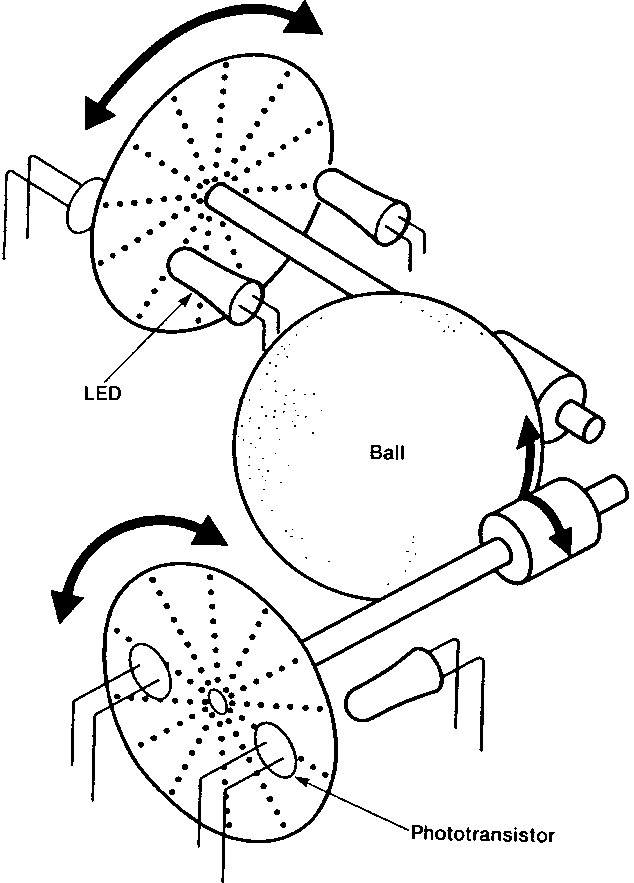
\includegraphics[width=0.3\linewidth]{theory_mech/2.1.png}
    \caption{Механическая мышь с шариком и роликами}
    \label{fig:theoryBallOpt}
\end{figure}

\begin{figure}[h]
    \centering
    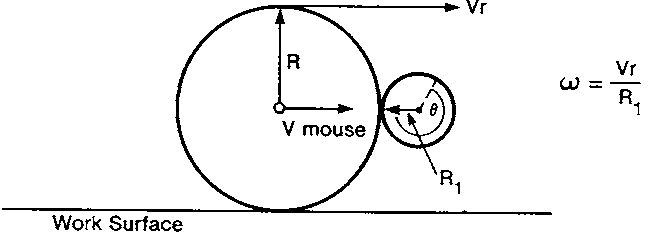
\includegraphics[width=0.3\linewidth]{theory_mech/2.2.png}
    \caption{Шар и ролик}
    \label{fig:theoryBallRoll}
\end{figure}

Мыши, которые используют шар для определения движения, могут быть представлены системой, показанной на рисунке \ref{fig:theoryBallRoll}. Скорость окружности шара $V_r$, равна скорости мыши, $V$. Так как ролик не прикреплен непосредственно к оси шара, а опирается на его окружность, при условии отсутствия проскальзывания скорость окружности ролика равна скорости окружности шара. Угловая скорость и вращение ролика теперь связаны с движением мыши с помощью приведенных выше уравнений, но радиус $R$ теперь намного меньше, и вал вращается намного быстрее.

$$\omega = V/R_1$$

\noindent где $V$ -- скорость мыши, а $R_1$ -- радиус ролика. Поскольку ролик меньше радиусом, он вращается быстрее при заданной скорости мыши.

Движение передается на датчики следующим образом. Ролики, которые прямо или косвенно вращаются колесом или шаром, подключены непосредственно к датчикам движения.

%\section{Оптомеханические мыши} \label{title:OptoMechanical}

Оптомеханические мыши для генерации квадратурных сигналов A и B используют устройство, называемое оптическим прерывателем. Как показано на рисунке \ref{fig:theoryQuadEncoder}, оптомеханическая система состоит из источника света (обычно светодиода), фотоприемника и оптического прерывателя, который соединен с вращающимся роликом мыши.

Прерыватель имеет серию чередующихся черных и белых полос, которые позволяют свету от светодиода попадать на детектор. Поскольку прерыватель вращается поперек линии светового луча, сплошные сегменты, расположенные между щелями, будут прерывать луч, и на выходе детектора появится серия импульсов напряжения. Второй квадратурный выход получается при использовании второго светодиода и детектора, которые смещены относительно первого светодиода и детектора на одну четверть угла радиальных прорезенй, или при использовании прорезей, которые смещены на одну четверть их периода, аналогично смещенным проводящим сегментам коммутатора. Маска с двумя сквозными отверстиями может использоваться с коммутатором, чтобы световые лучи находились в квадратуре относительно вращения прерывателя. Маска может быть просверлена или выполнена методом литья так, чтобы отверстия различались по фазе точно на 90 градусов.

\begin{figure}[h]
    \centering
    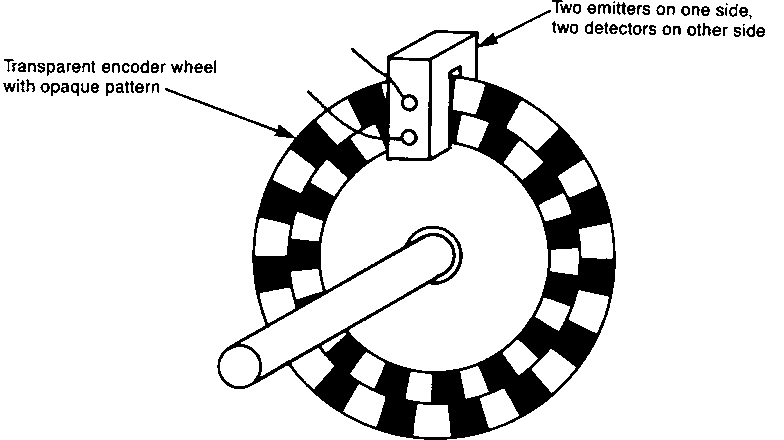
\includegraphics[width=0.5\linewidth]{theory_mech/2.76.PNG}
    \caption{Оптический энкодер с квадратурными выходами}
    \label{fig:theoryQuadEncoder}
\end{figure}

\begin{figure}[h]
    \centering
    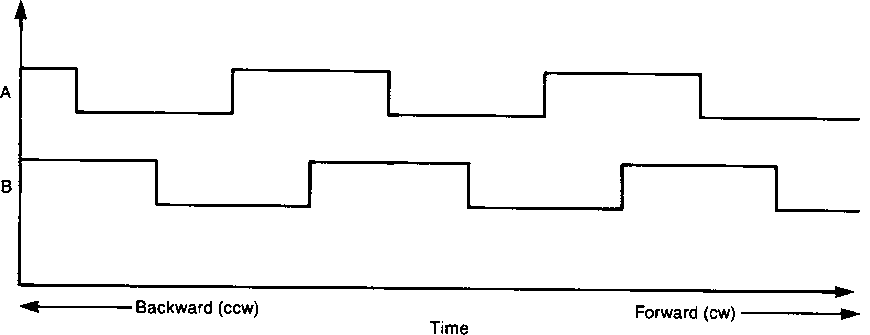
\includegraphics[width=0.5\linewidth]{theory_mech/2.77.PNG}
    \caption{Квадратурные сигналы}
    \label{fig:theoryQuadDiag}
\end{figure}

Выход оптического энкодера представляет собой два квадратурных сигнала, как показано на рисунке \ref{fig:theoryQuadDiag}. Направление можно определить, изучив соотношение фаз двух сигналов. Если сигнал A находится в состоянии высокого уровня, когда на сигнале B возникает восходящий фронт, то движение происходит в прямом направлении. Если микропроцессор достаточно быстр, сигналы могут быть подключены непосредственно к входному порту, а все декодирование и подсчет выполняются в программном обеспечении.

\end{document}

\documentclass[11pt, a4paper]{article}
\usepackage{pdfpages}
\usepackage{parallel}
\usepackage[T2A]{fontenc}
\usepackage{ucs}
\usepackage[utf8x]{inputenc}
\usepackage[polish,english,russian]{babel}
\usepackage{hyperref}
\usepackage{rotating}
\usepackage[inner=2cm,top=1.8cm,outer=2cm,bottom=2.3cm,nohead]{geometry}
\usepackage{listings}
\usepackage{graphicx}
\usepackage{wrapfig}
\usepackage{longtable}
\usepackage{indentfirst}
\usepackage{array}
\usepackage{tikzsymbols}
\usepackage{soul}
\usepackage[ruled,vlined]{algorithm2e}
%\counterwithout{figure}{section} 

\usepackage{url}
\makeatletter
\g@addto@macro{\UrlBreaks}{\UrlOrds}
\makeatother

\newcolumntype{P}[1]{>{\raggedright\arraybackslash}p{#1}}
\frenchspacing
\usepackage{fixltx2e} %text sub- and superscripts
\usepackage{icomma} % коскі ў матэматычным рэжыме
\PreloadUnicodePage{4}

\newcommand{\longpage}{\enlargethispage{\baselineskip}}
\newcommand{\shortpage}{\enlargethispage{-\baselineskip}}

\def\switchlang#1{\expandafter\csname switchlang#1\endcsname}
\def\switchlangbe{
\let\saverefname=\refname%
\def\refname{Літаратура}%
\def\figurename{Іл.}%
}
\def\switchlangen{
\let\saverefname=\refname%
\def\refname{References}%
\def\figurename{Fig.}%
}
\def\switchlangru{
\let\saverefname=\refname%
\let\savefigurename=\figurename%
\def\refname{Литература}%
\def\figurename{Рис.}%
}

\hyphenation{admi-ni-stra-tive}
\hyphenation{ex-pe-ri-ence}
\hyphenation{fle-xi-bi-li-ty}
\hyphenation{Py-thon}
\hyphenation{ma-the-ma-ti-cal}
\hyphenation{re-ported}
\hyphenation{imp-le-menta-tions}
\hyphenation{pro-vides}
\hyphenation{en-gi-neering}
\hyphenation{com-pa-ti-bi-li-ty}
\hyphenation{im-pos-sible}
\hyphenation{desk-top}
\hyphenation{elec-tro-nic}
\hyphenation{com-pa-ny}
\hyphenation{de-ve-lop-ment}
\hyphenation{de-ve-loping}
\hyphenation{de-ve-lop}
\hyphenation{da-ta-ba-se}
\hyphenation{plat-forms}
\hyphenation{or-ga-ni-za-tion}
\hyphenation{pro-gramming}
\hyphenation{in-stru-ments}
\hyphenation{Li-nux}
\hyphenation{sour-ce}
\hyphenation{en-vi-ron-ment}
\hyphenation{Te-le-pathy}
\hyphenation{Li-nux-ov-ka}
\hyphenation{Open-BSD}
\hyphenation{Free-BSD}
\hyphenation{men-ti-on-ed}
\hyphenation{app-li-ca-tion}

\def\progref!#1!{\texttt{#1}}
\renewcommand{\arraystretch}{2} %Іначай формулы ў матрыцы зліпаюцца з лініямі
\usepackage{array}

\def\interview #1 (#2), #3, #4, #5\par{

\section[#1, #3, #4]{#1 -- #3, #4}
\def\qname{LVEE}
\def\aname{#1}
\def\q ##1\par{{\noindent \bf \qname: ##1 }\par}
\def\a{{\noindent \bf \aname: } \def\qname{L}\def\aname{#2}}
}

\def\interview* #1 (#2), #3, #4, #5\par{

\section*{#1\\{\small\rm #3, #4. #5}}
\ifx\ParallelWhichBox\undefined%
    \addcontentsline{toc}{section}{#1, #3, #4}%
\else%
\ifnum\ParallelWhichBox=0%
    \addcontentsline{toc}{section}{#1, #3, #4}%
\fi\fi%

\def\qname{LVEE}
\def\aname{#1}
\def\q ##1\par{{\noindent \bf \qname: ##1 }\par}
\def\a{{\noindent \bf \aname: } \def\qname{L}\def\aname{#2}}
}

\newcommand{\interviewfooter}[1]{
\vskip 1em
\noindent \textit{#1}
}


\begin{document}

\title{Трекбол}

\maketitle

    Трекбол используется для тех же целей, что и мышь. Его внутренняя конструкция почти идентична мыши и может рассматриваться как перевернутая мышь, находящаяся в неподвижном положении. Трекбол исторически предшествовал мыши, и существует версия, что концепция мыши была придумана в ходе переворачивания трекбола вверх ногами и перемещения его по поверхности стола. Основные характеристики трекбола показаны на рисунке \ref{fig:theoryTrackballGeneric}. Трекбол представляет собой металлический или пластиковый шар, который монтируется в раме так, что только небольшая его часть выступает через отверстие в верхней части рамы. Шар поддерживается двумя ортогональными роликами-стержнями, так что, когда шар поворачивается влево или вправо, вращается один ролик, а когда он поворачивается вперед или назад, вращается другой.
    
    \begin{figure}[h]
        \centering
    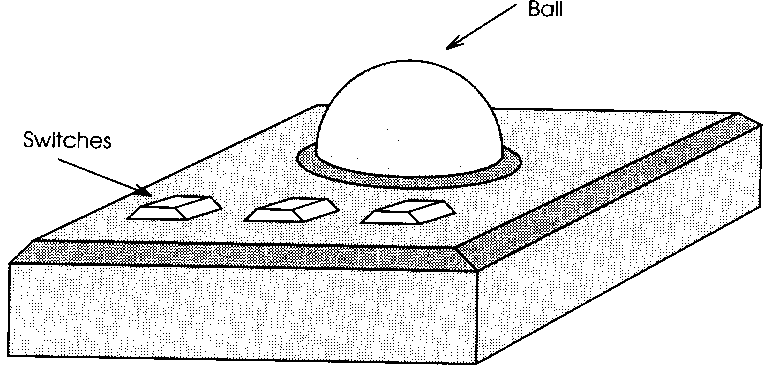
\includegraphics[width=0.5\linewidth]{theory_track/2.3.png}
        \caption{Трекбол}
        \label{fig:theoryTrackballGeneric}
    \end{figure}
    
    Шар полностью свободно вращается в своем гнезде. Он управляется ладонью руки, и движения, принимаемые шаром, находящимся в контакте с двумя роликами, преобразуются внутри корпуса так же, как у механической мыши. Движения роликов так же детектируются путем измерения вращения дисков, прикрепленных к их концам. Это детектирование может выполняться с помощью электрических контактов или светодиодов и фотоприемников.
    
    Как и мышь, трекбол обычно включает в себя несколько кнопок, до которых можно дотянуться кончиками пальцев, пока ладонь лежит на шаре. Для большинства целей мышь более популярна, чем трекбол, но в ситуациях, когда недостаточно свободного места или нет подходящей поверхности, трекбол оказывается более предпочтительным.

\end{document}

\documentclass[11pt, a4paper]{article}
\usepackage{pdfpages}
\usepackage{parallel}
\usepackage[T2A]{fontenc}
\usepackage{ucs}
\usepackage[utf8x]{inputenc}
\usepackage[polish,english,russian]{babel}
\usepackage{hyperref}
\usepackage{rotating}
\usepackage[inner=2cm,top=1.8cm,outer=2cm,bottom=2.3cm,nohead]{geometry}
\usepackage{listings}
\usepackage{graphicx}
\usepackage{wrapfig}
\usepackage{longtable}
\usepackage{indentfirst}
\usepackage{array}
\usepackage{tikzsymbols}
\usepackage{soul}
\usepackage[ruled,vlined]{algorithm2e}
%\counterwithout{figure}{section} 

\usepackage{url}
\makeatletter
\g@addto@macro{\UrlBreaks}{\UrlOrds}
\makeatother

\newcolumntype{P}[1]{>{\raggedright\arraybackslash}p{#1}}
\frenchspacing
\usepackage{fixltx2e} %text sub- and superscripts
\usepackage{icomma} % коскі ў матэматычным рэжыме
\PreloadUnicodePage{4}

\newcommand{\longpage}{\enlargethispage{\baselineskip}}
\newcommand{\shortpage}{\enlargethispage{-\baselineskip}}

\def\switchlang#1{\expandafter\csname switchlang#1\endcsname}
\def\switchlangbe{
\let\saverefname=\refname%
\def\refname{Літаратура}%
\def\figurename{Іл.}%
}
\def\switchlangen{
\let\saverefname=\refname%
\def\refname{References}%
\def\figurename{Fig.}%
}
\def\switchlangru{
\let\saverefname=\refname%
\let\savefigurename=\figurename%
\def\refname{Литература}%
\def\figurename{Рис.}%
}

\hyphenation{admi-ni-stra-tive}
\hyphenation{ex-pe-ri-ence}
\hyphenation{fle-xi-bi-li-ty}
\hyphenation{Py-thon}
\hyphenation{ma-the-ma-ti-cal}
\hyphenation{re-ported}
\hyphenation{imp-le-menta-tions}
\hyphenation{pro-vides}
\hyphenation{en-gi-neering}
\hyphenation{com-pa-ti-bi-li-ty}
\hyphenation{im-pos-sible}
\hyphenation{desk-top}
\hyphenation{elec-tro-nic}
\hyphenation{com-pa-ny}
\hyphenation{de-ve-lop-ment}
\hyphenation{de-ve-loping}
\hyphenation{de-ve-lop}
\hyphenation{da-ta-ba-se}
\hyphenation{plat-forms}
\hyphenation{or-ga-ni-za-tion}
\hyphenation{pro-gramming}
\hyphenation{in-stru-ments}
\hyphenation{Li-nux}
\hyphenation{sour-ce}
\hyphenation{en-vi-ron-ment}
\hyphenation{Te-le-pathy}
\hyphenation{Li-nux-ov-ka}
\hyphenation{Open-BSD}
\hyphenation{Free-BSD}
\hyphenation{men-ti-on-ed}
\hyphenation{app-li-ca-tion}

\def\progref!#1!{\texttt{#1}}
\renewcommand{\arraystretch}{2} %Іначай формулы ў матрыцы зліпаюцца з лініямі
\usepackage{array}

\def\interview #1 (#2), #3, #4, #5\par{

\section[#1, #3, #4]{#1 -- #3, #4}
\def\qname{LVEE}
\def\aname{#1}
\def\q ##1\par{{\noindent \bf \qname: ##1 }\par}
\def\a{{\noindent \bf \aname: } \def\qname{L}\def\aname{#2}}
}

\def\interview* #1 (#2), #3, #4, #5\par{

\section*{#1\\{\small\rm #3, #4. #5}}
\ifx\ParallelWhichBox\undefined%
    \addcontentsline{toc}{section}{#1, #3, #4}%
\else%
\ifnum\ParallelWhichBox=0%
    \addcontentsline{toc}{section}{#1, #3, #4}%
\fi\fi%

\def\qname{LVEE}
\def\aname{#1}
\def\q ##1\par{{\noindent \bf \qname: ##1 }\par}
\def\a{{\noindent \bf \aname: } \def\qname{L}\def\aname{#2}}
}

\newcommand{\interviewfooter}[1]{
\vskip 1em
\noindent \textit{#1}
}


\begin{document}

\title{1987 "--- MicroSpeed FastTRAP trackball}
\date{}
\maketitle

Устройство FastTRAP от MicroSpeed, выпущенное в 1987 году, представляет собой трекбол с тремя кнопками, а также дополнительным колесом, благодаря которому он может выдавать координаты не по двум, а по трем координатным осям  — \textit{x}, \textit{y} и \textit{z} — то есть поддерживает на одну координатную плоскость больше, чем мышь или планшет. Дополнительная ось была рассчитана в первую очередь на пользователей САПР твердотельного моделирования, поскольку именно в них одновременное изменение сразу в трёх координатных осях может сократить время, необходимое для вращения объекта или проекции в окне просмотра.

\begin{figure}[h]
   \centering
    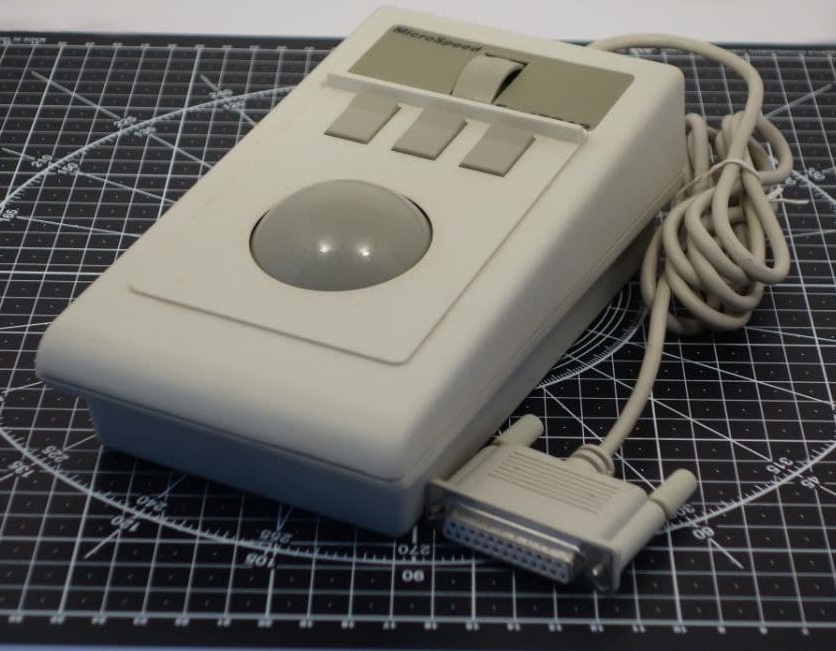
\includegraphics[scale=0.3]{1987_microspeed_fasttrap/fast.jpg}
    \caption{Изображение FastTRAP  на размерном коврике}
    \label{fig:FastTRAPSize}
\end{figure}

Управление по оси \textit{z} осуществляется вращением колеса; однако в момент выпуска этого устройства концепции колеса прокрутки еще не существовало, поэтому программное обеспечение не позволяет использовать его для скроллинга в графических или текстовых программах.

\begin{figure}[h]
    \centering
    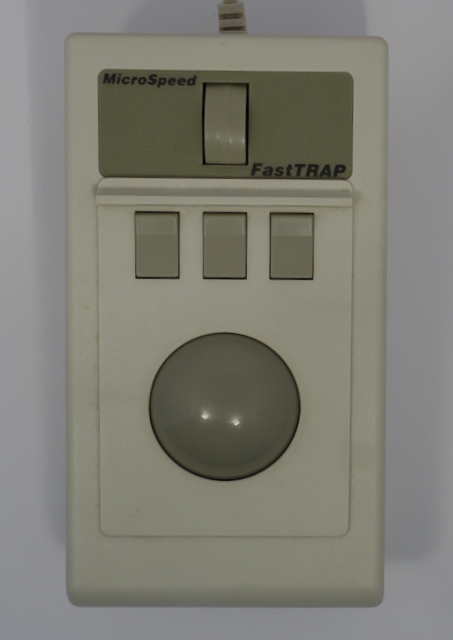
\includegraphics[scale=0.3]{1987_microspeed_fasttrap/fast3.png}
    \caption{Изображение FastTRAP, вид сверху}
    \label{fig:FastTRAPTop}
\end{figure}

При подключении к компьютеру FastTRAP использует протокол мыши Microsoft, и может использовать соответствующий стандартный драйвер. Идущий в комплекте специализированный драйвер требуется только для работы с третьей координатой. Также идущая в комплекте программа настройки позволяет запрограммировать функции клавиш, шара и колеса, что позволяет адаптировать устройство под любое программное обеспечение: например выполнять определенные команды DOS \cite{fast}.

В плане эргономики кнопки трекбола расположены достаточно удобно в плане досягаемости "--- при условии, что пользователь накрывает шар ладонью. Однако колесо нахоидится на противоположном от пользователя краю корпуса, и для его вращения пользователю может понадобиться перемещать руку (рис. \ref{fig:FastTRAPHand}).

\begin{figure}[h]
    \centering
    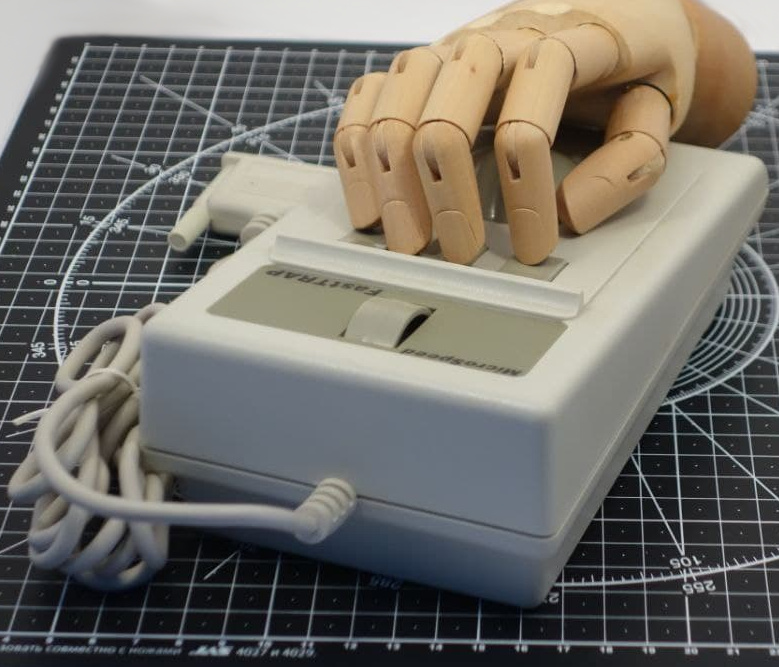
\includegraphics[scale=0.25]{1987_microspeed_fasttrap/fast1.jpg}
    \caption{Изображение FastTRAP на размерном коврике с моделью руки человека}
    \label{fig:FastTRAPHand}
\end{figure}

Помимо третьей координаты, FastTRAP предоставляет пользователям САПР дополнительное преимущество за счет большого диаметра шара: точное размещение курсора в графическом окне оказывается точнее проще, чем при перемещении мыши в нужное положение (иногда не удается избежать случайного перемещения мыши при нажатии кнопки).

\begin{figure}[h]
    \centering
    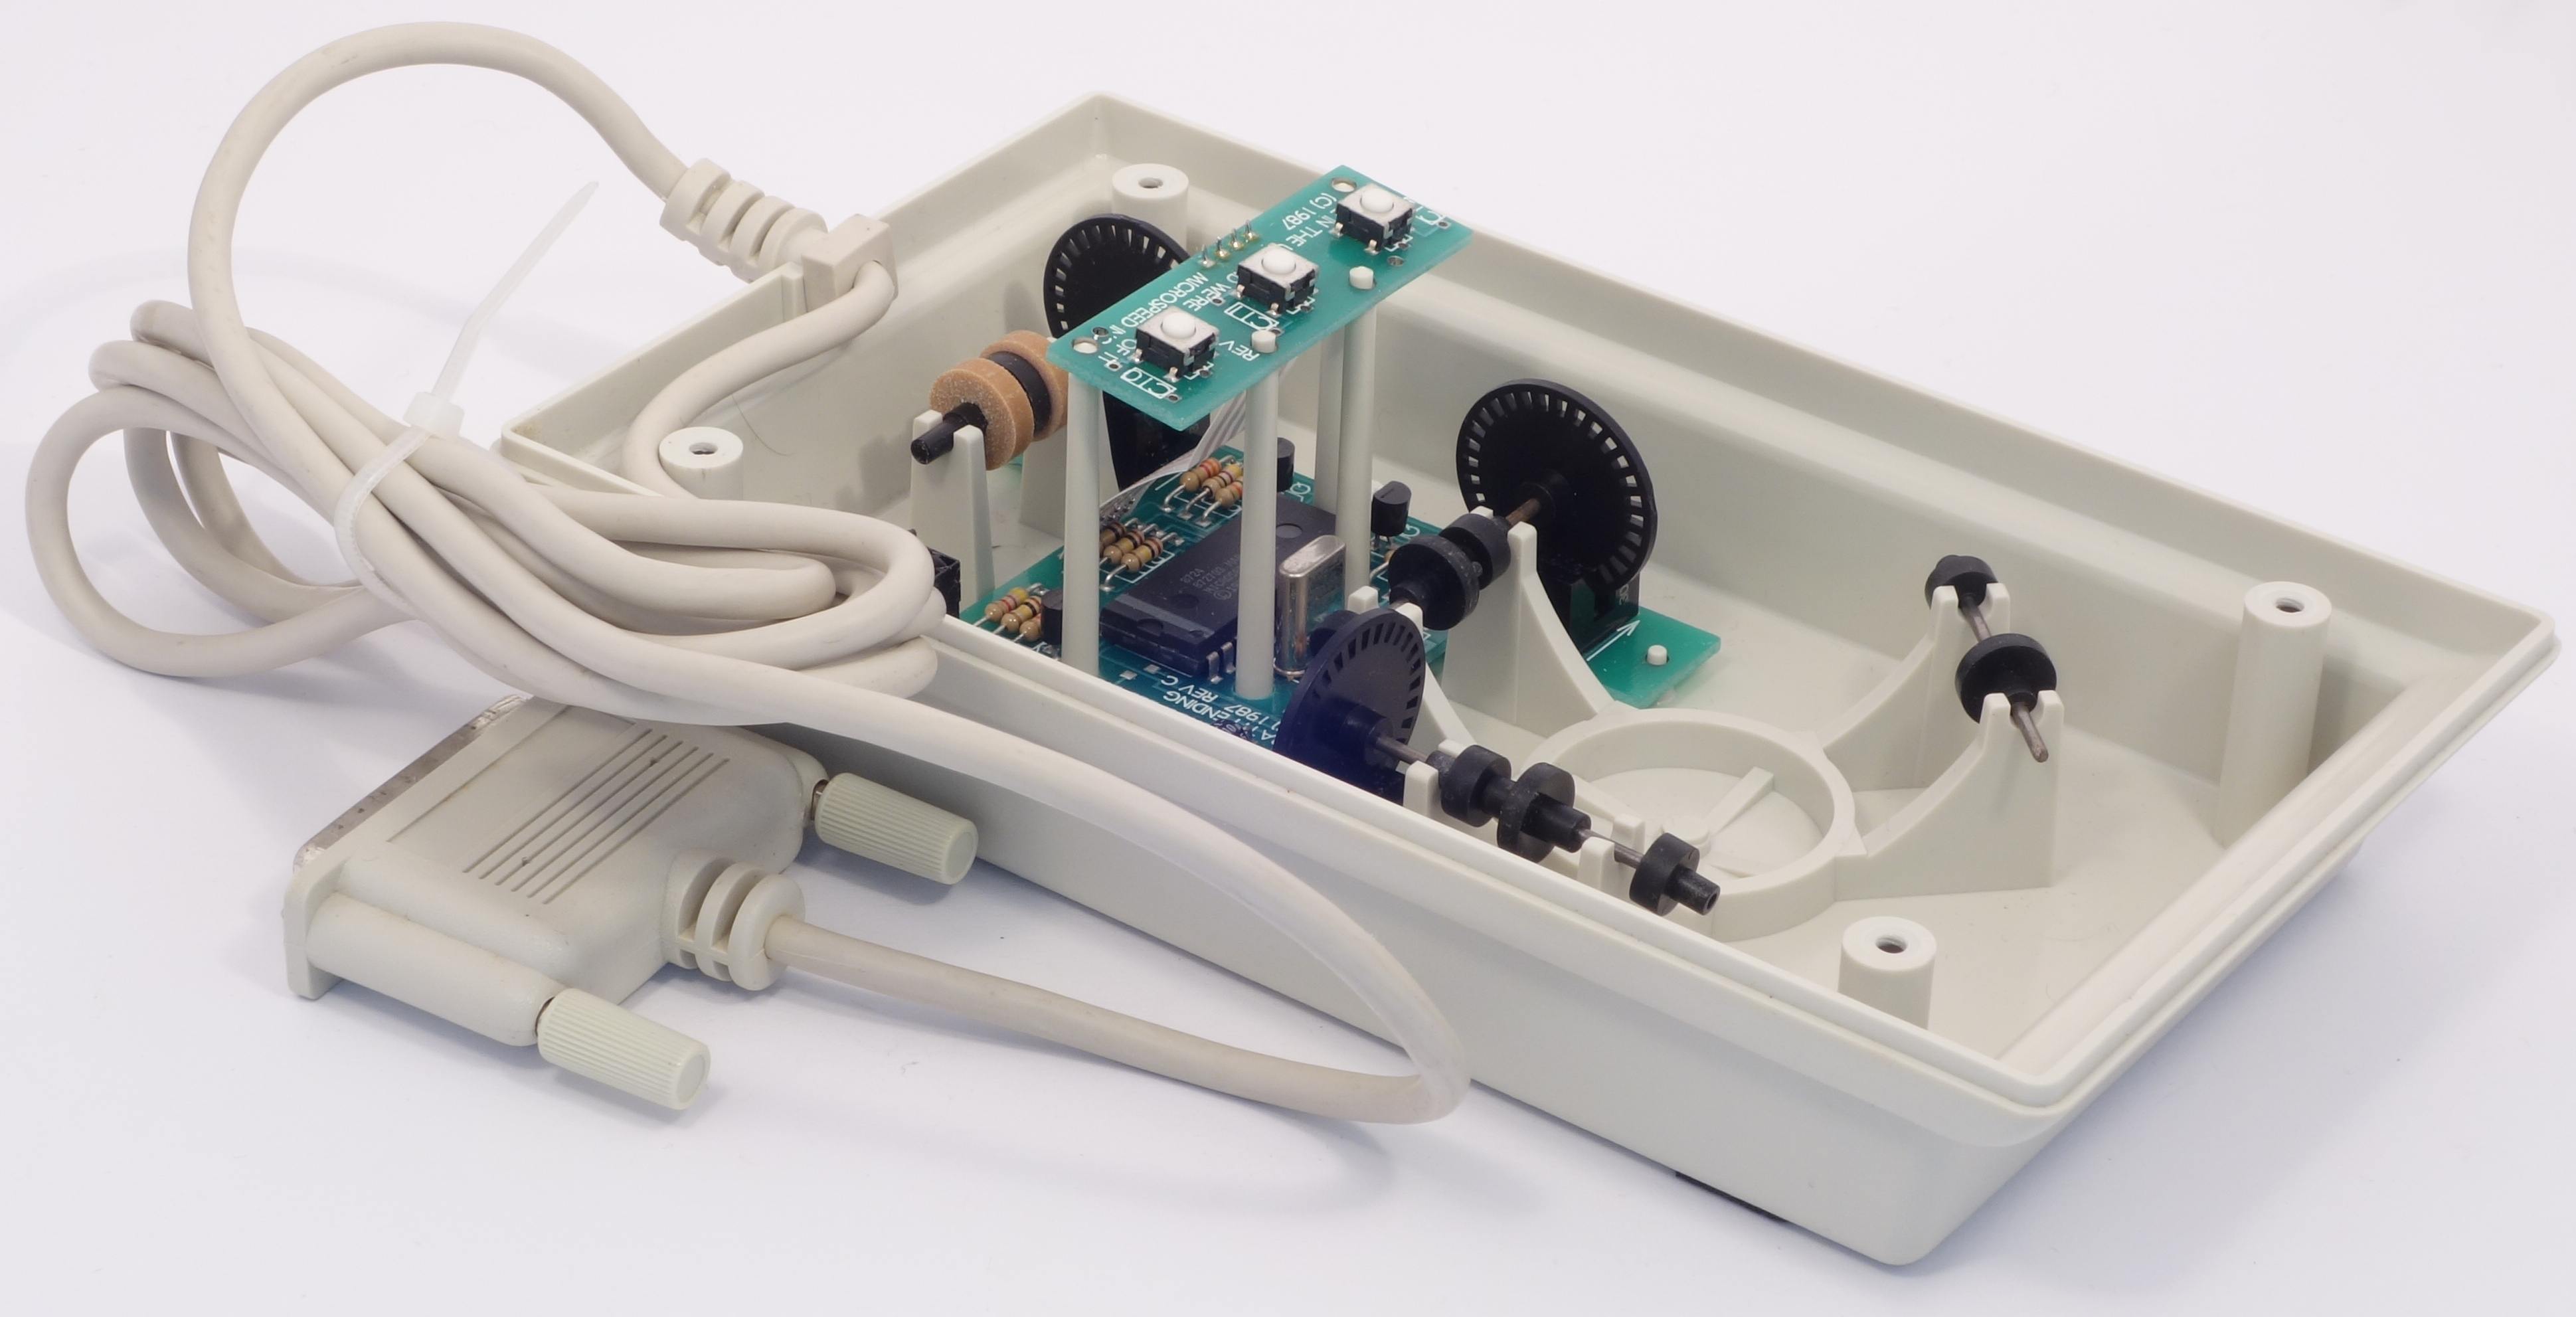
\includegraphics[scale=0.5]{1987_microspeed_fasttrap/sony.jpg}
    \caption{Изображение FastTRAP в разобранном виде}
    \label{fig:FastTRAPInside}
\end{figure}

Внутреннее устройство трекбола можно видеть на рис. \ref{fig:FastTRAPInside}.
Стандартная оптомеханическая конструкция дополнена фрикционной передачей, связывающей ролик с дополнительным оптомеханическим энкодером. Также можно заметить идентичность энкодеров, выполняющих снятие перемещения по всем трём осям: с одной стороны, это оказалось не самой сложной задачей в плане компоновки (учитывая большие размеры корпуса), а с другой, это может быть актуальным, учитывая назначение дополнительного колеса.

\begin{thebibliography}{9}
\bibitem {fast} G. Kunkel. The 3-D FastTRAP points with precision // PC Magazine, November 24, 19987. - p. 56.
\end{thebibliography}
\end{document}

\documentclass[11pt, a4paper]{article}
\usepackage{pdfpages}
\usepackage{parallel}
\usepackage[T2A]{fontenc}
\usepackage{ucs}
\usepackage[utf8x]{inputenc}
\usepackage[polish,english,russian]{babel}
\usepackage{hyperref}
\usepackage{rotating}
\usepackage[inner=2cm,top=1.8cm,outer=2cm,bottom=2.3cm,nohead]{geometry}
\usepackage{listings}
\usepackage{graphicx}
\usepackage{wrapfig}
\usepackage{longtable}
\usepackage{indentfirst}
\usepackage{array}
\usepackage{tikzsymbols}
\usepackage{soul}
\usepackage[ruled,vlined]{algorithm2e}
%\counterwithout{figure}{section} 

\usepackage{url}
\makeatletter
\g@addto@macro{\UrlBreaks}{\UrlOrds}
\makeatother

\newcolumntype{P}[1]{>{\raggedright\arraybackslash}p{#1}}
\frenchspacing
\usepackage{fixltx2e} %text sub- and superscripts
\usepackage{icomma} % коскі ў матэматычным рэжыме
\PreloadUnicodePage{4}

\newcommand{\longpage}{\enlargethispage{\baselineskip}}
\newcommand{\shortpage}{\enlargethispage{-\baselineskip}}

\def\switchlang#1{\expandafter\csname switchlang#1\endcsname}
\def\switchlangbe{
\let\saverefname=\refname%
\def\refname{Літаратура}%
\def\figurename{Іл.}%
}
\def\switchlangen{
\let\saverefname=\refname%
\def\refname{References}%
\def\figurename{Fig.}%
}
\def\switchlangru{
\let\saverefname=\refname%
\let\savefigurename=\figurename%
\def\refname{Литература}%
\def\figurename{Рис.}%
}

\hyphenation{admi-ni-stra-tive}
\hyphenation{ex-pe-ri-ence}
\hyphenation{fle-xi-bi-li-ty}
\hyphenation{Py-thon}
\hyphenation{ma-the-ma-ti-cal}
\hyphenation{re-ported}
\hyphenation{imp-le-menta-tions}
\hyphenation{pro-vides}
\hyphenation{en-gi-neering}
\hyphenation{com-pa-ti-bi-li-ty}
\hyphenation{im-pos-sible}
\hyphenation{desk-top}
\hyphenation{elec-tro-nic}
\hyphenation{com-pa-ny}
\hyphenation{de-ve-lop-ment}
\hyphenation{de-ve-loping}
\hyphenation{de-ve-lop}
\hyphenation{da-ta-ba-se}
\hyphenation{plat-forms}
\hyphenation{or-ga-ni-za-tion}
\hyphenation{pro-gramming}
\hyphenation{in-stru-ments}
\hyphenation{Li-nux}
\hyphenation{sour-ce}
\hyphenation{en-vi-ron-ment}
\hyphenation{Te-le-pathy}
\hyphenation{Li-nux-ov-ka}
\hyphenation{Open-BSD}
\hyphenation{Free-BSD}
\hyphenation{men-ti-on-ed}
\hyphenation{app-li-ca-tion}

\def\progref!#1!{\texttt{#1}}
\renewcommand{\arraystretch}{2} %Іначай формулы ў матрыцы зліпаюцца з лініямі
\usepackage{array}

\def\interview #1 (#2), #3, #4, #5\par{

\section[#1, #3, #4]{#1 -- #3, #4}
\def\qname{LVEE}
\def\aname{#1}
\def\q ##1\par{{\noindent \bf \qname: ##1 }\par}
\def\a{{\noindent \bf \aname: } \def\qname{L}\def\aname{#2}}
}

\def\interview* #1 (#2), #3, #4, #5\par{

\section*{#1\\{\small\rm #3, #4. #5}}
\ifx\ParallelWhichBox\undefined%
    \addcontentsline{toc}{section}{#1, #3, #4}%
\else%
\ifnum\ParallelWhichBox=0%
    \addcontentsline{toc}{section}{#1, #3, #4}%
\fi\fi%

\def\qname{LVEE}
\def\aname{#1}
\def\q ##1\par{{\noindent \bf \qname: ##1 }\par}
\def\a{{\noindent \bf \aname: } \def\qname{L}\def\aname{#2}}
}

\newcommand{\interviewfooter}[1]{
\vskip 1em
\noindent \textit{#1}
}


\begin{document}

\title{1989 "--- Prohance PowerMouse}
\date{}
\maketitle

Мышь Prohance была выпущенна компание Prohance Technologies inc. в 1989 году в рамках целого смемейства из нескольких мышей и одного трекбола, ориентированных на пользователей электронных таблиц Lotus 1-2-3 (и некоторых других подобных приложений). Концепция Prohance заключается в размещении множества дополнительных кнопок на корпусе, которые, по замыслу разработчиков, избавляют пользователя от необходимости часто перемещать руку с мыши на клавиатуру и обратно. Prohance mouse содержит в переденй части корпуса дополнительную функциональную клавиатуру: в данной модели присутствует 10 функциональных кнопок (рис. \ref{fig:ProhancePhoto}), а вообще их число могло доходить до 40 (что реализовывалось благодаря сильно вытянутому в длину корпусу мыши, похожему на пульт дистанционного управления).

\begin{figure}[h]
    \centering
    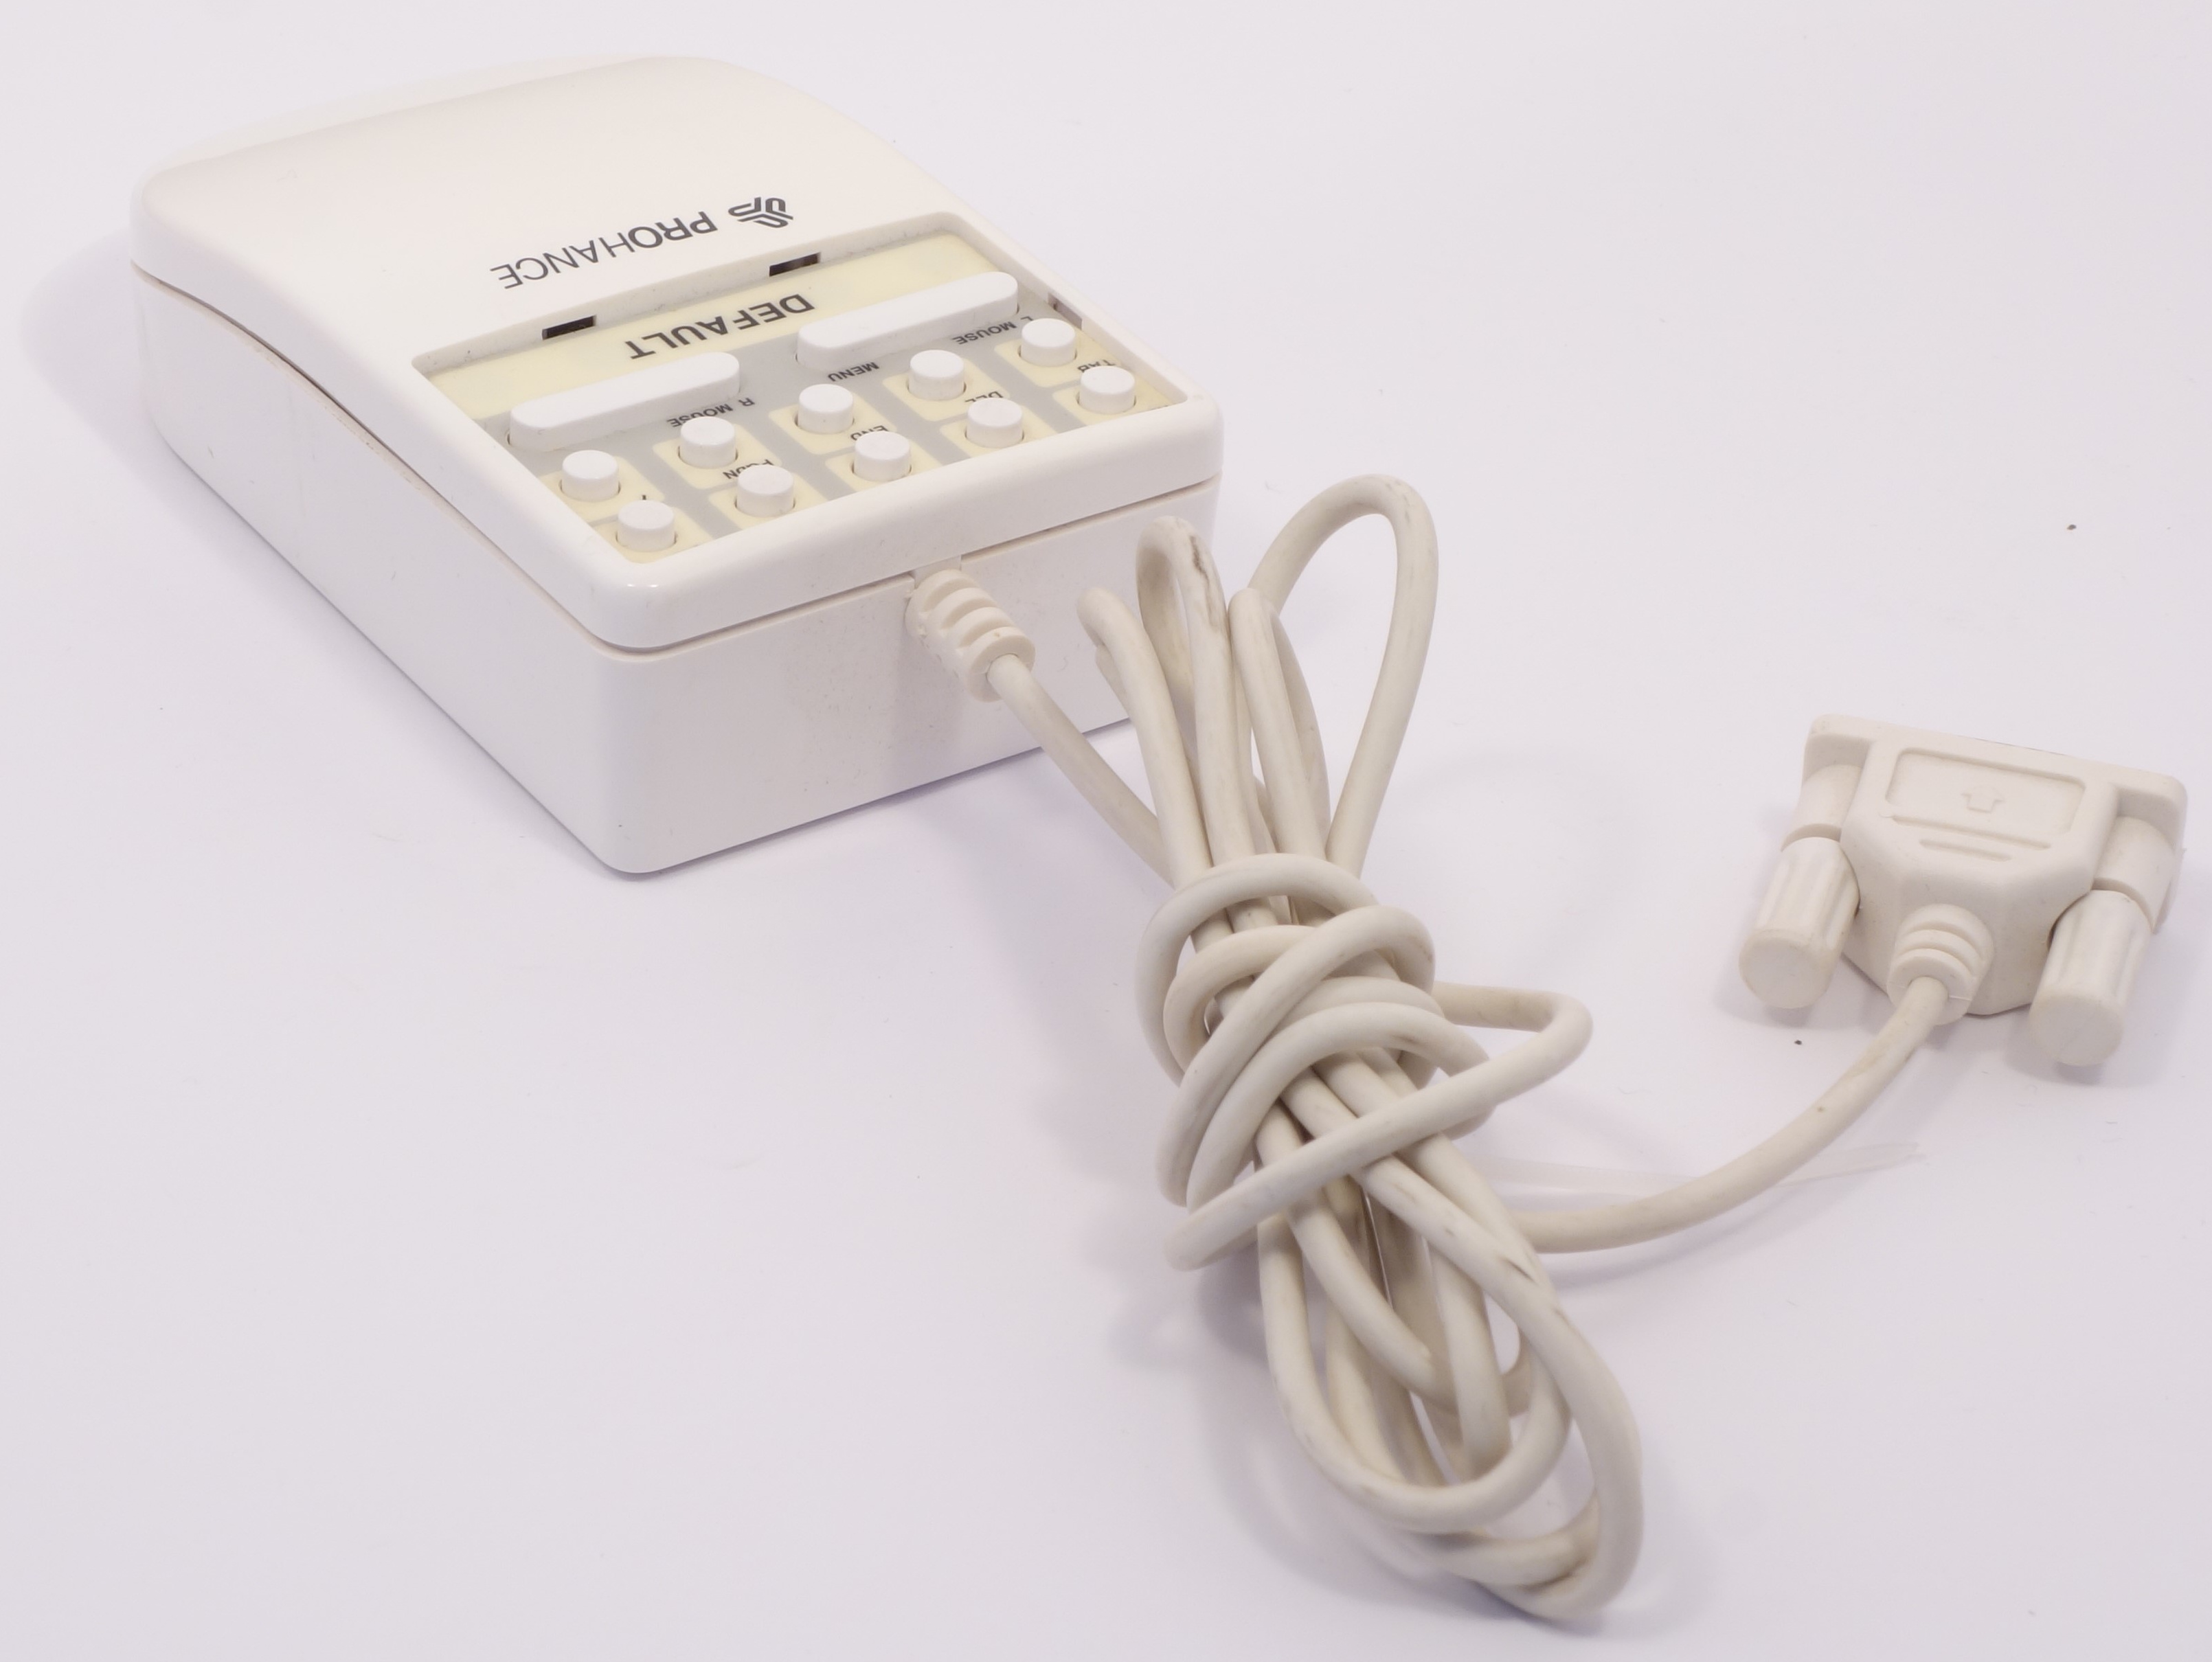
\includegraphics[scale=0.4]{1989_prohance_powermouse/5.1jpg.jpg}
    \caption{Изображение Prohance mouse}
    \label{fig:ProhancePhoto}
\end{figure}

Смысл использования данной мыши при работе с электронными таблицами Lotus 1-2-3 сводится к тому, что каждой функциональной клавише соответствует некая последовательность клавиатурных кодов, то есть фактически нажатие приводит к выполнению заданной макрокоманды. В остальном этот манипулятор действует как любая другая мышь, что позволяет использовать его с любыми графическими программами.

В плане эргономики корпус данного конкретного манипулятора повторяет форму мыши Microsoft, известной как <<Dove Bar mouse>>, в свою очередь позаимствовавшей форму у шлифовального бруска, и потому оказавшейся одной из первых эргономичных мышшей (рис. \ref{fig:ProhanceSize}). 

\begin{figure}[h]
    \centering
    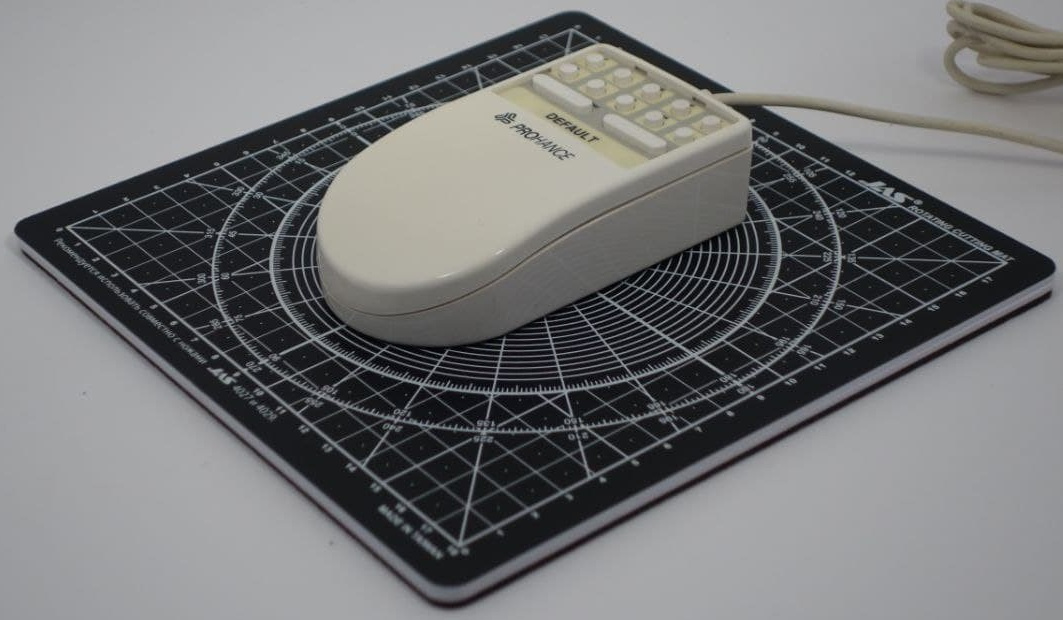
\includegraphics[scale=0.3]{1989_prohance_powermouse/5.3.jpg}
    \caption{Изображение Prohance Mouse на размерном коврике с шагом сетки 1~см}
    \label{fig:ProhanceSize}
\end{figure}

Поэтому с точки зрения формы к Prohance PoverMouse нет претензий по части эргономики (в отличие от её старшего собрата PowerMouse 100 с его сорока функциональными клавишами). Однако важным недостатком является размер клавиш: как основные кнопки, так и дополнительные клавиши Prohance имеют очень маленькую площадь, что весьма невыгодно отличает их от похожей по форме мыши Microsoft. Колпачки клавиш резиновые, как у микрокалькулятора, и издают едва слышный клик при нажатии. При этом они имеют некоторый запас хода, поэтому вероятность случайного срабатывания мала.

Сами по себе колпачки кнопок не содержат тактильных или визуальных отличительных признаков. Это особенно проблемно для функциональных клавиш: они имеют круглые колпачки одинакового размера, поэтому перед нажатием нужно внимательно следить за правильным положением пальцев. Для идентификации клавиш предусмотрены сменные вставки - накладки, размещаемые поверх функциональной клавиатуры. Однако из-за размера мыши эти надписи достаточно мелкие, перекрываются пальцами, и нетренированному пользователю приходится пристально их рассматривать, чтобы найти нужную (разница в размерах подушечки пальца и функциональной кнопки хорошо видна на рис. \ref{fig:ProhanceHand}).

\begin{figure}[h]
    \centering
    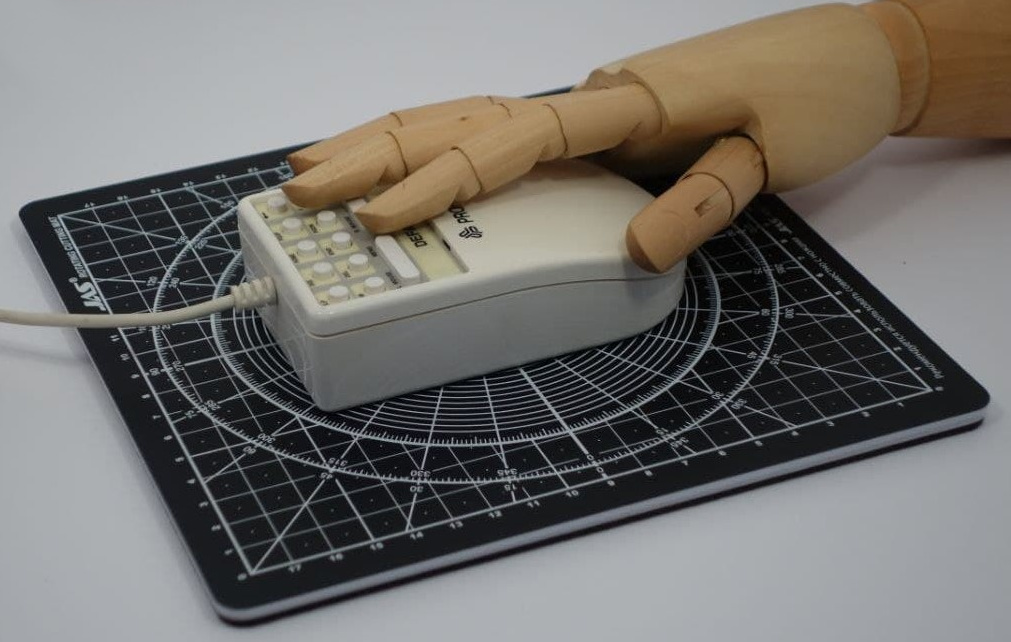
\includegraphics[scale=0.3]{1989_prohance_powermouse/5.2.jpg}
    \caption{Изображение Prohance Mouse с моделью руки человека}
    \label{fig:ProhanceHand}
\end{figure}

Поэтому в целом Prohance PowerMouse получала негативные отзывы пользователей, вынужденных нажимать на чрезвычайно узкие левую и правую кнопки мыши, и вглядываться в мелкие надписи между рядами функциональных клавиш.

В \ref{prohance} отмечается, что в ранней версии драйвера содержались ошибки, приводившие к неадекватной работе мыши в Microsoft Word (даже ее незначительное перемещение приводило к пролистыванию страниц), исправленные в обновленной версии. Также отмечалась некоторая программная несовместимость с драйвером мыши Microsoft, приводившая к неработоспособности мыши в части приложений.

При этом настройка Prohance через комплектное программное обеспечение достаточно простая. В отличие от других мышей того времени, у Prohance нет программно реализованных экранных меню "--- вместо этого предлагается использовать переназначение функциональных клавиш. Prohance предоставляет функцию записи макросов, которая позволяет определять новые шаблоны для ее функциональных клавиш, а также изменять существующие.
Драйвер также позволяет задавать через конфигурационный файл уровень чувствительности мыши, однако функция динамического регулирования ускорения мыши предусмотрена не была.

\begin{figure}[h]
    \centering
    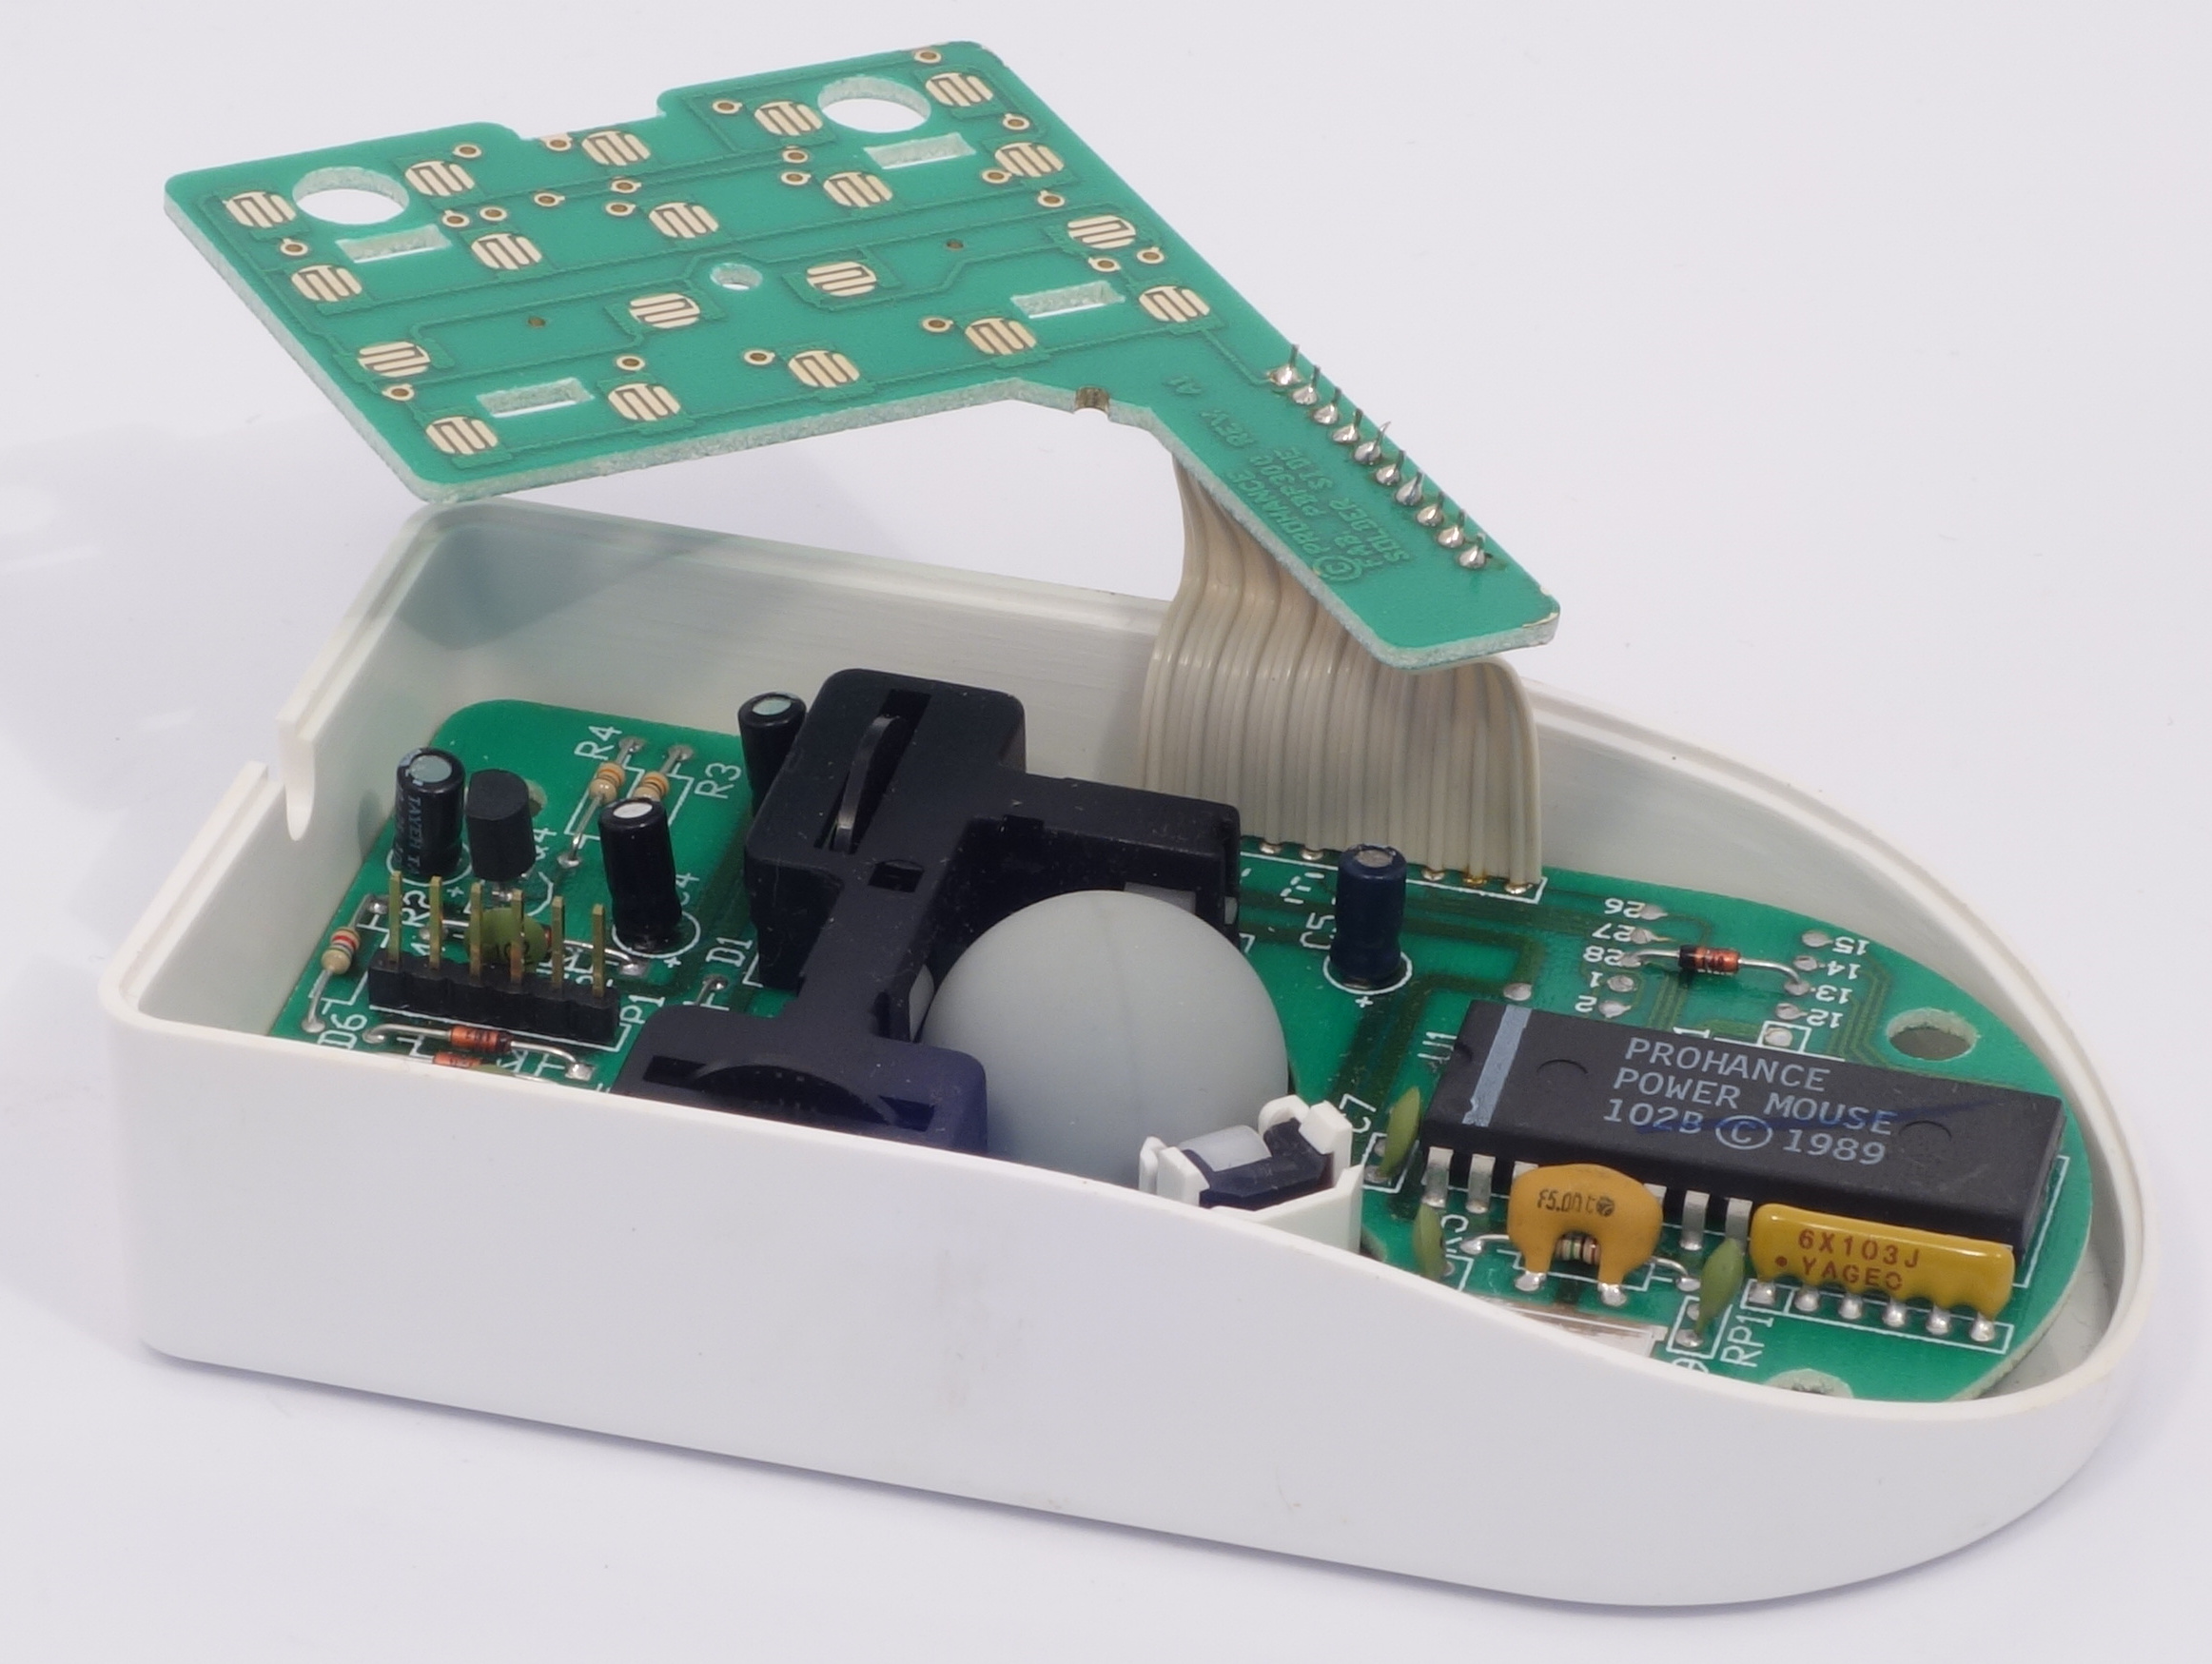
\includegraphics[scale=0.8]{1989_prohance_powermouse/6.1.jpg}
    \caption{Изображение Prohance в разобранном виде}
    \label{fig:ProhanceInside}
\end{figure}

Мышь в разобранном виде показана на рис. \ref{fig:ProhanceInside}. Как можно видеть, она представляет собой типичную для 90-х годов оптомеханическую конструкцию, а блок кнопок и функциональных клавиш выполнен на отдельной печатной плате и является миниатюрной мембранной клавиатурой, аналогичной устанавливаемым в карманных микрокалькуляторах.

\begin{thebibliography}{9}
\bibitem{prohance} Gruman G. What price mice? // Infoworld, V. 12, No. 17, April 23, 1990. - P. 63-69.
\bibitem{livingston} Livingston B. Genetically engineered mice run amok at Windows World // InfoWorld, Vol. 15, Iss. 21, May 24, 1989. - p. 34. \url{https://books.google.by/books?id=PTsEAAAAMBAJ&lpg=PA34&dq=prohance%20mouse&hl=ru&pg=PA34#v=onepage&q=prohance%20mouse&f=false}
\end{thebibliography}
\end{document}

\documentclass[11pt, a4paper]{article}
\usepackage{pdfpages}
\usepackage{parallel}
\usepackage[T2A]{fontenc}
\usepackage{ucs}
\usepackage[utf8x]{inputenc}
\usepackage[polish,english,russian]{babel}
\usepackage{hyperref}
\usepackage{rotating}
\usepackage[inner=2cm,top=1.8cm,outer=2cm,bottom=2.3cm,nohead]{geometry}
\usepackage{listings}
\usepackage{graphicx}
\usepackage{wrapfig}
\usepackage{longtable}
\usepackage{indentfirst}
\usepackage{array}
\usepackage{tikzsymbols}
\usepackage{soul}
\usepackage[ruled,vlined]{algorithm2e}
%\counterwithout{figure}{section} 

\usepackage{url}
\makeatletter
\g@addto@macro{\UrlBreaks}{\UrlOrds}
\makeatother

\newcolumntype{P}[1]{>{\raggedright\arraybackslash}p{#1}}
\frenchspacing
\usepackage{fixltx2e} %text sub- and superscripts
\usepackage{icomma} % коскі ў матэматычным рэжыме
\PreloadUnicodePage{4}

\newcommand{\longpage}{\enlargethispage{\baselineskip}}
\newcommand{\shortpage}{\enlargethispage{-\baselineskip}}

\def\switchlang#1{\expandafter\csname switchlang#1\endcsname}
\def\switchlangbe{
\let\saverefname=\refname%
\def\refname{Літаратура}%
\def\figurename{Іл.}%
}
\def\switchlangen{
\let\saverefname=\refname%
\def\refname{References}%
\def\figurename{Fig.}%
}
\def\switchlangru{
\let\saverefname=\refname%
\let\savefigurename=\figurename%
\def\refname{Литература}%
\def\figurename{Рис.}%
}

\hyphenation{admi-ni-stra-tive}
\hyphenation{ex-pe-ri-ence}
\hyphenation{fle-xi-bi-li-ty}
\hyphenation{Py-thon}
\hyphenation{ma-the-ma-ti-cal}
\hyphenation{re-ported}
\hyphenation{imp-le-menta-tions}
\hyphenation{pro-vides}
\hyphenation{en-gi-neering}
\hyphenation{com-pa-ti-bi-li-ty}
\hyphenation{im-pos-sible}
\hyphenation{desk-top}
\hyphenation{elec-tro-nic}
\hyphenation{com-pa-ny}
\hyphenation{de-ve-lop-ment}
\hyphenation{de-ve-loping}
\hyphenation{de-ve-lop}
\hyphenation{da-ta-ba-se}
\hyphenation{plat-forms}
\hyphenation{or-ga-ni-za-tion}
\hyphenation{pro-gramming}
\hyphenation{in-stru-ments}
\hyphenation{Li-nux}
\hyphenation{sour-ce}
\hyphenation{en-vi-ron-ment}
\hyphenation{Te-le-pathy}
\hyphenation{Li-nux-ov-ka}
\hyphenation{Open-BSD}
\hyphenation{Free-BSD}
\hyphenation{men-ti-on-ed}
\hyphenation{app-li-ca-tion}

\def\progref!#1!{\texttt{#1}}
\renewcommand{\arraystretch}{2} %Іначай формулы ў матрыцы зліпаюцца з лініямі
\usepackage{array}

\def\interview #1 (#2), #3, #4, #5\par{

\section[#1, #3, #4]{#1 -- #3, #4}
\def\qname{LVEE}
\def\aname{#1}
\def\q ##1\par{{\noindent \bf \qname: ##1 }\par}
\def\a{{\noindent \bf \aname: } \def\qname{L}\def\aname{#2}}
}

\def\interview* #1 (#2), #3, #4, #5\par{

\section*{#1\\{\small\rm #3, #4. #5}}
\ifx\ParallelWhichBox\undefined%
    \addcontentsline{toc}{section}{#1, #3, #4}%
\else%
\ifnum\ParallelWhichBox=0%
    \addcontentsline{toc}{section}{#1, #3, #4}%
\fi\fi%

\def\qname{LVEE}
\def\aname{#1}
\def\q ##1\par{{\noindent \bf \qname: ##1 }\par}
\def\a{{\noindent \bf \aname: } \def\qname{L}\def\aname{#2}}
}

\newcommand{\interviewfooter}[1]{
\vskip 1em
\noindent \textit{#1}
}


\begin{document}

\title{1989 "--- Kraft trackball}
\date{}
\maketitle

Kraft trackball, известный также как Kraft TripleTrack \cite{triple} "---	 это трекбол, разработанный в конце 80-х годов компанией Kraft Systems, и выпускавшийся для нескольких семейств компьютеров: IBM PC, Atari ST, Commodore 64 и Amiga. К особенностям трекбола можно отнести переключатель блокировки кнопок для выбора и дополнительную съемную педаль.

\begin{figure}[h]
    \centering
    \includegraphics[scale=0.4]{1989_kraft_trackball/pic_30.jpg}
    \caption{Изображение Kraft trackball}
    \label{fig:KraftPhoto}
\end{figure}

Kraft trackball имеет симметричный корпус, и поэтому подходит как для левшей, так и для правшей. Три кнопки расположены на ближней к пользователю части устройства, поэтому трекбол не предлагает никакой опоры под запястье. Центральная кнопка действует как стандартная правая кнопка мыши. Кнопки построены на основе качественных переключателями с различимым кликом; однако из-за достаточно большого хода колпачки кнопок при нажатии уходят вглубь, из-за чего их сложнее нажимать большим пальцем.

\begin{figure}[h]
    \centering
    \includegraphics[scale=0.25]{1989_kraft_trackball/size_30.jpg}
    \caption{Изображение Kraft trackball на размерном коврике с шагом сетки 1~см}
    \label{fig:KraftSize}
\end{figure}

Шар имеет хорошую подвижность, поэтому проблем в управлении курсором у устройства нет. При этом часть с шаром несколько приподнята над кнопками, что можно расценивать в плане эргономики как преимущество.

В \cite{Hudnall} отмечается простота установки идущего в комплекте программного обеспечения, а также выделены две проблемы в управлении курсором с помощью этого трекбола: кнопки нажимаются сложнее, чем, например, кнопки у популярных моделей мышей, а также иногда происходит проскальзывание шара (курсор остается на месте). Последняя проблема решается пользователем с помощью быстрого возвратно-поступательного движения. В целом, поместив средний палец на шар, а большой палец на крайнюю левую кнопку (рис. \ref{fig:KraftHand}), получается довольно легко перемещать курсор по экрану. Использование правой или средней кнопки менее естественно в анатомическом плане, к нему сложнее привыкнуть, и, к счастью для пользователя, в конце восьмидесятых годов это требовалось не так часто.

\begin{figure}[h]
    \centering
    \includegraphics[scale=0.25]{1989_kraft_trackball/hand_30.jpg}
    \caption{Изображение Kraft trackball с моделью руки человека}
    \label{fig:KraftHand}
\end{figure}

Для облегчения операций перетаскивания объектов, а также выделения текста кликом и перетаскиванием, на устройстве предусмотрена четвертая кнопка, расположенная позади шара слева. Она срабатывает как левая кнопка, но реализована на базе переключателя с фиксацией, поэтому блокируется в нажатом состоянии до следующего нажатия. Расположение этой кнопки позволяет предположить что она рассчитана на нажатие указательным пальцем. Учитывая расположение, маленький размер и форму, нажимали ее не так часто.

Наиболее уникальным дополнительным аксессуаром трекбола Kraft является ножная педаль (рис. \ref{fig:KraftPedal}). Она подключатеся к трекболу сзади с помощью стандартного телефонного кабеля с разъёмом RJ-11, и представляет собой прочный прямоугольник высотой в 1.5, шириной в 2 и длиной в 4 дюйма. Нажатие на педаль аналогично нажатию левой кнопки трекбола. Согласно обзору, представленному в \cite{kraftwithpedal}, в реальной эксплуатации педаль может практически полностью заменить левую кнопку.

\begin{figure}[h]
    \centering
    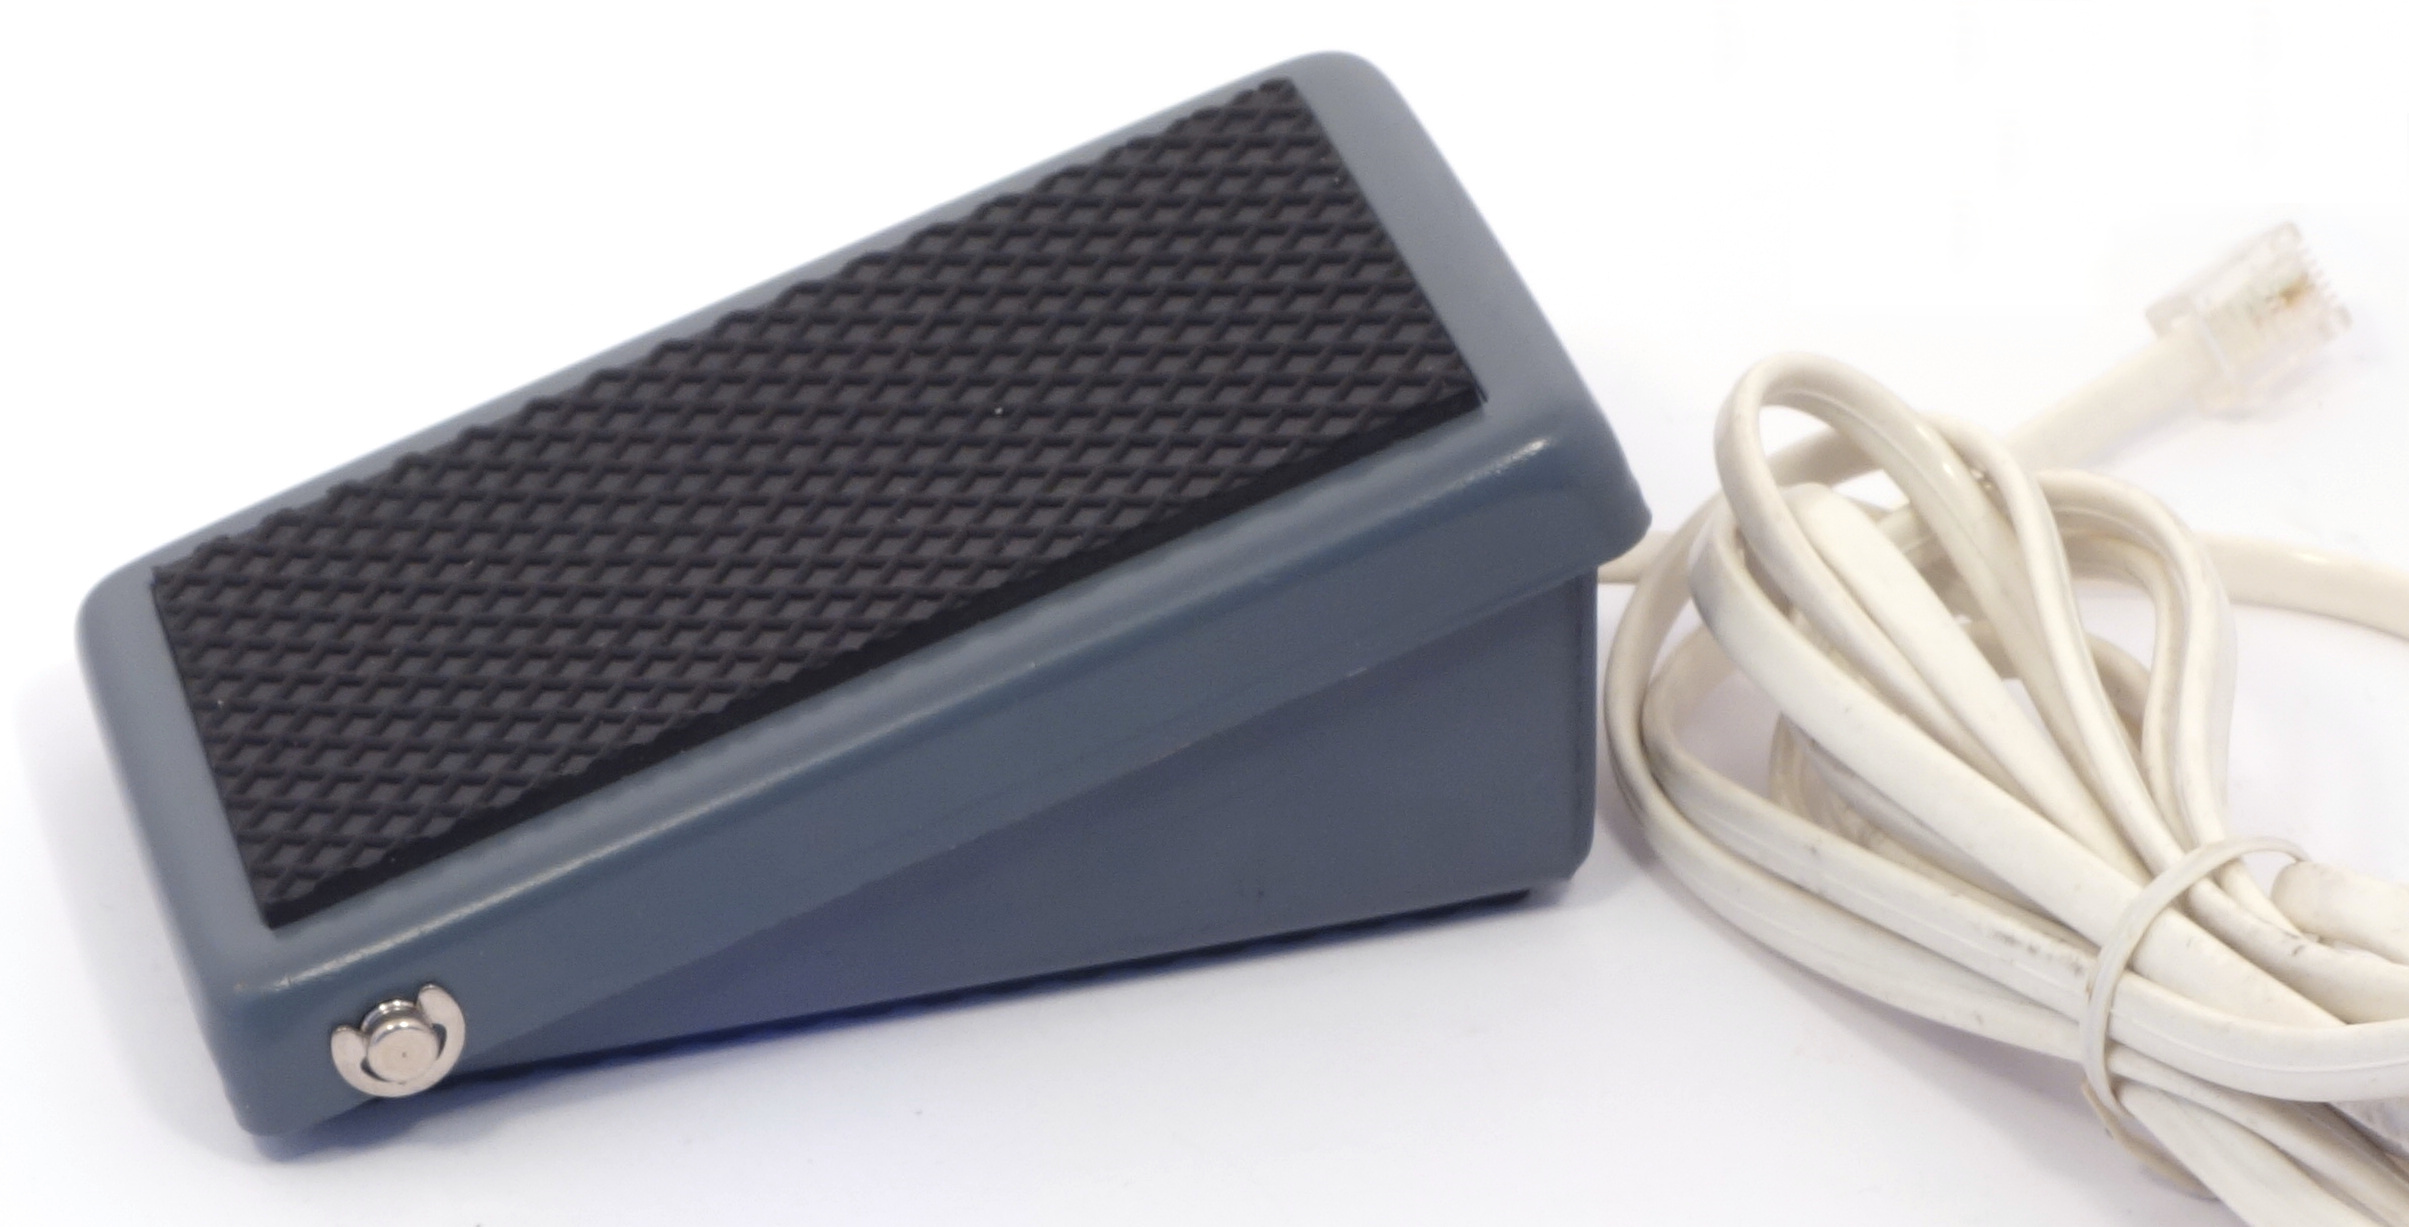
\includegraphics[scale=0.4]{1990_kraft_toptrack/pedal_30.jpg}
    \caption{Педаль Kraft trackball}
    \label{fig:KraftPedal}
\end{figure}

Вид трекбола в разобранном виде показан на рисунке \ref{fig:KraftInside}. Как можно видеть, технически это станадртное устройство позиционирования, выполненное по оптомеханической схеме. Проверка кода по базе данных Федеральной комиссии по коммуникациям США подтверждает, что трекбол был разработан американской компанией Kraft Systems в 1989 году.

\begin{figure}[h]
    \centering
    \includegraphics[scale=0.6]{1989_kraft_trackball/inside_30.jpg}
    \caption{Изображение Kraft trackball в разобранном виде}
    \label{fig:KraftInside}
\end{figure}

Программное обеспечение, поставляемое с трекболом, позволяет использовать его как с приложениями, управляемыми мышью, так и с приложениями, рассчитанными на управление с помощью клавиатуры. Драйвер позволяет настроить скорость, распознавание последовательных портов и некоторые другие элементы. Кроме того, трекбол Kraft можно использовать как с 9-контактным, так и с 25-контактным разъемом \cite{Hudnall}.

\begin{thebibliography}{9}
\bibitem{triple} Lennard V. Trackball Round-Up. ATARI/P\&G/CONTRIVER/MCS/MARCONI/KRAFT Trackballs // Music technology, December 1990. -- P. 42--47. \url{http://www.muzines.co.uk/articles/trackball-round-up/462}

\bibitem{Hudnall} Hudnall M. Kraft Trackball // Compute, August 1991. - P. 42. \url{https://www.atarimagazines.com/compute/issue132/42_Kraft_Trackball.php}

\bibitem{kraftwithpedal} Unger T. Kraft Trackball // PC Magazine, V. 9, No. 14, August 1990. - P. 249-251. \url{https://books.google.by/books?id=cSMUxSP5pKgC&lpg=PT255&dq=kraft%20trackball&pg=PT255#v=onepage&q&f=false}
\end{thebibliography}
\end{document} 

\documentclass[11pt, a4paper]{article}
\usepackage{pdfpages}
\usepackage{parallel}
\usepackage[T2A]{fontenc}
\usepackage{ucs}
\usepackage[utf8x]{inputenc}
\usepackage[polish,english,russian]{babel}
\usepackage{hyperref}
\usepackage{rotating}
\usepackage[inner=2cm,top=1.8cm,outer=2cm,bottom=2.3cm,nohead]{geometry}
\usepackage{listings}
\usepackage{graphicx}
\usepackage{wrapfig}
\usepackage{longtable}
\usepackage{indentfirst}
\usepackage{array}
\usepackage{tikzsymbols}
\usepackage{soul}
\usepackage[ruled,vlined]{algorithm2e}
%\counterwithout{figure}{section} 

\usepackage{url}
\makeatletter
\g@addto@macro{\UrlBreaks}{\UrlOrds}
\makeatother

\newcolumntype{P}[1]{>{\raggedright\arraybackslash}p{#1}}
\frenchspacing
\usepackage{fixltx2e} %text sub- and superscripts
\usepackage{icomma} % коскі ў матэматычным рэжыме
\PreloadUnicodePage{4}

\newcommand{\longpage}{\enlargethispage{\baselineskip}}
\newcommand{\shortpage}{\enlargethispage{-\baselineskip}}

\def\switchlang#1{\expandafter\csname switchlang#1\endcsname}
\def\switchlangbe{
\let\saverefname=\refname%
\def\refname{Літаратура}%
\def\figurename{Іл.}%
}
\def\switchlangen{
\let\saverefname=\refname%
\def\refname{References}%
\def\figurename{Fig.}%
}
\def\switchlangru{
\let\saverefname=\refname%
\let\savefigurename=\figurename%
\def\refname{Литература}%
\def\figurename{Рис.}%
}

\hyphenation{admi-ni-stra-tive}
\hyphenation{ex-pe-ri-ence}
\hyphenation{fle-xi-bi-li-ty}
\hyphenation{Py-thon}
\hyphenation{ma-the-ma-ti-cal}
\hyphenation{re-ported}
\hyphenation{imp-le-menta-tions}
\hyphenation{pro-vides}
\hyphenation{en-gi-neering}
\hyphenation{com-pa-ti-bi-li-ty}
\hyphenation{im-pos-sible}
\hyphenation{desk-top}
\hyphenation{elec-tro-nic}
\hyphenation{com-pa-ny}
\hyphenation{de-ve-lop-ment}
\hyphenation{de-ve-loping}
\hyphenation{de-ve-lop}
\hyphenation{da-ta-ba-se}
\hyphenation{plat-forms}
\hyphenation{or-ga-ni-za-tion}
\hyphenation{pro-gramming}
\hyphenation{in-stru-ments}
\hyphenation{Li-nux}
\hyphenation{sour-ce}
\hyphenation{en-vi-ron-ment}
\hyphenation{Te-le-pathy}
\hyphenation{Li-nux-ov-ka}
\hyphenation{Open-BSD}
\hyphenation{Free-BSD}
\hyphenation{men-ti-on-ed}
\hyphenation{app-li-ca-tion}

\def\progref!#1!{\texttt{#1}}
\renewcommand{\arraystretch}{2} %Іначай формулы ў матрыцы зліпаюцца з лініямі
\usepackage{array}

\def\interview #1 (#2), #3, #4, #5\par{

\section[#1, #3, #4]{#1 -- #3, #4}
\def\qname{LVEE}
\def\aname{#1}
\def\q ##1\par{{\noindent \bf \qname: ##1 }\par}
\def\a{{\noindent \bf \aname: } \def\qname{L}\def\aname{#2}}
}

\def\interview* #1 (#2), #3, #4, #5\par{

\section*{#1\\{\small\rm #3, #4. #5}}
\ifx\ParallelWhichBox\undefined%
    \addcontentsline{toc}{section}{#1, #3, #4}%
\else%
\ifnum\ParallelWhichBox=0%
    \addcontentsline{toc}{section}{#1, #3, #4}%
\fi\fi%

\def\qname{LVEE}
\def\aname{#1}
\def\q ##1\par{{\noindent \bf \qname: ##1 }\par}
\def\a{{\noindent \bf \aname: } \def\qname{L}\def\aname{#2}}
}

\newcommand{\interviewfooter}[1]{
\vskip 1em
\noindent \textit{#1}
}


\begin{document}

\title{1990 "--- Трекбол Kraft TopTrak}
\date{}
\maketitle

Трекбол TopTrak имеет средние размеры и корпус с закруглёнными углами (рис. \ref{fig:TopTrakTopAndBottom}). Устройство снабжено кабелем длиной 2,5 м, что заметно больше типового расстояния между пользователем и системным блоком. Трекбол имеет последовательный интерфейс сопряжения с компьютером.

\begin{figure}[h]
    \centering
    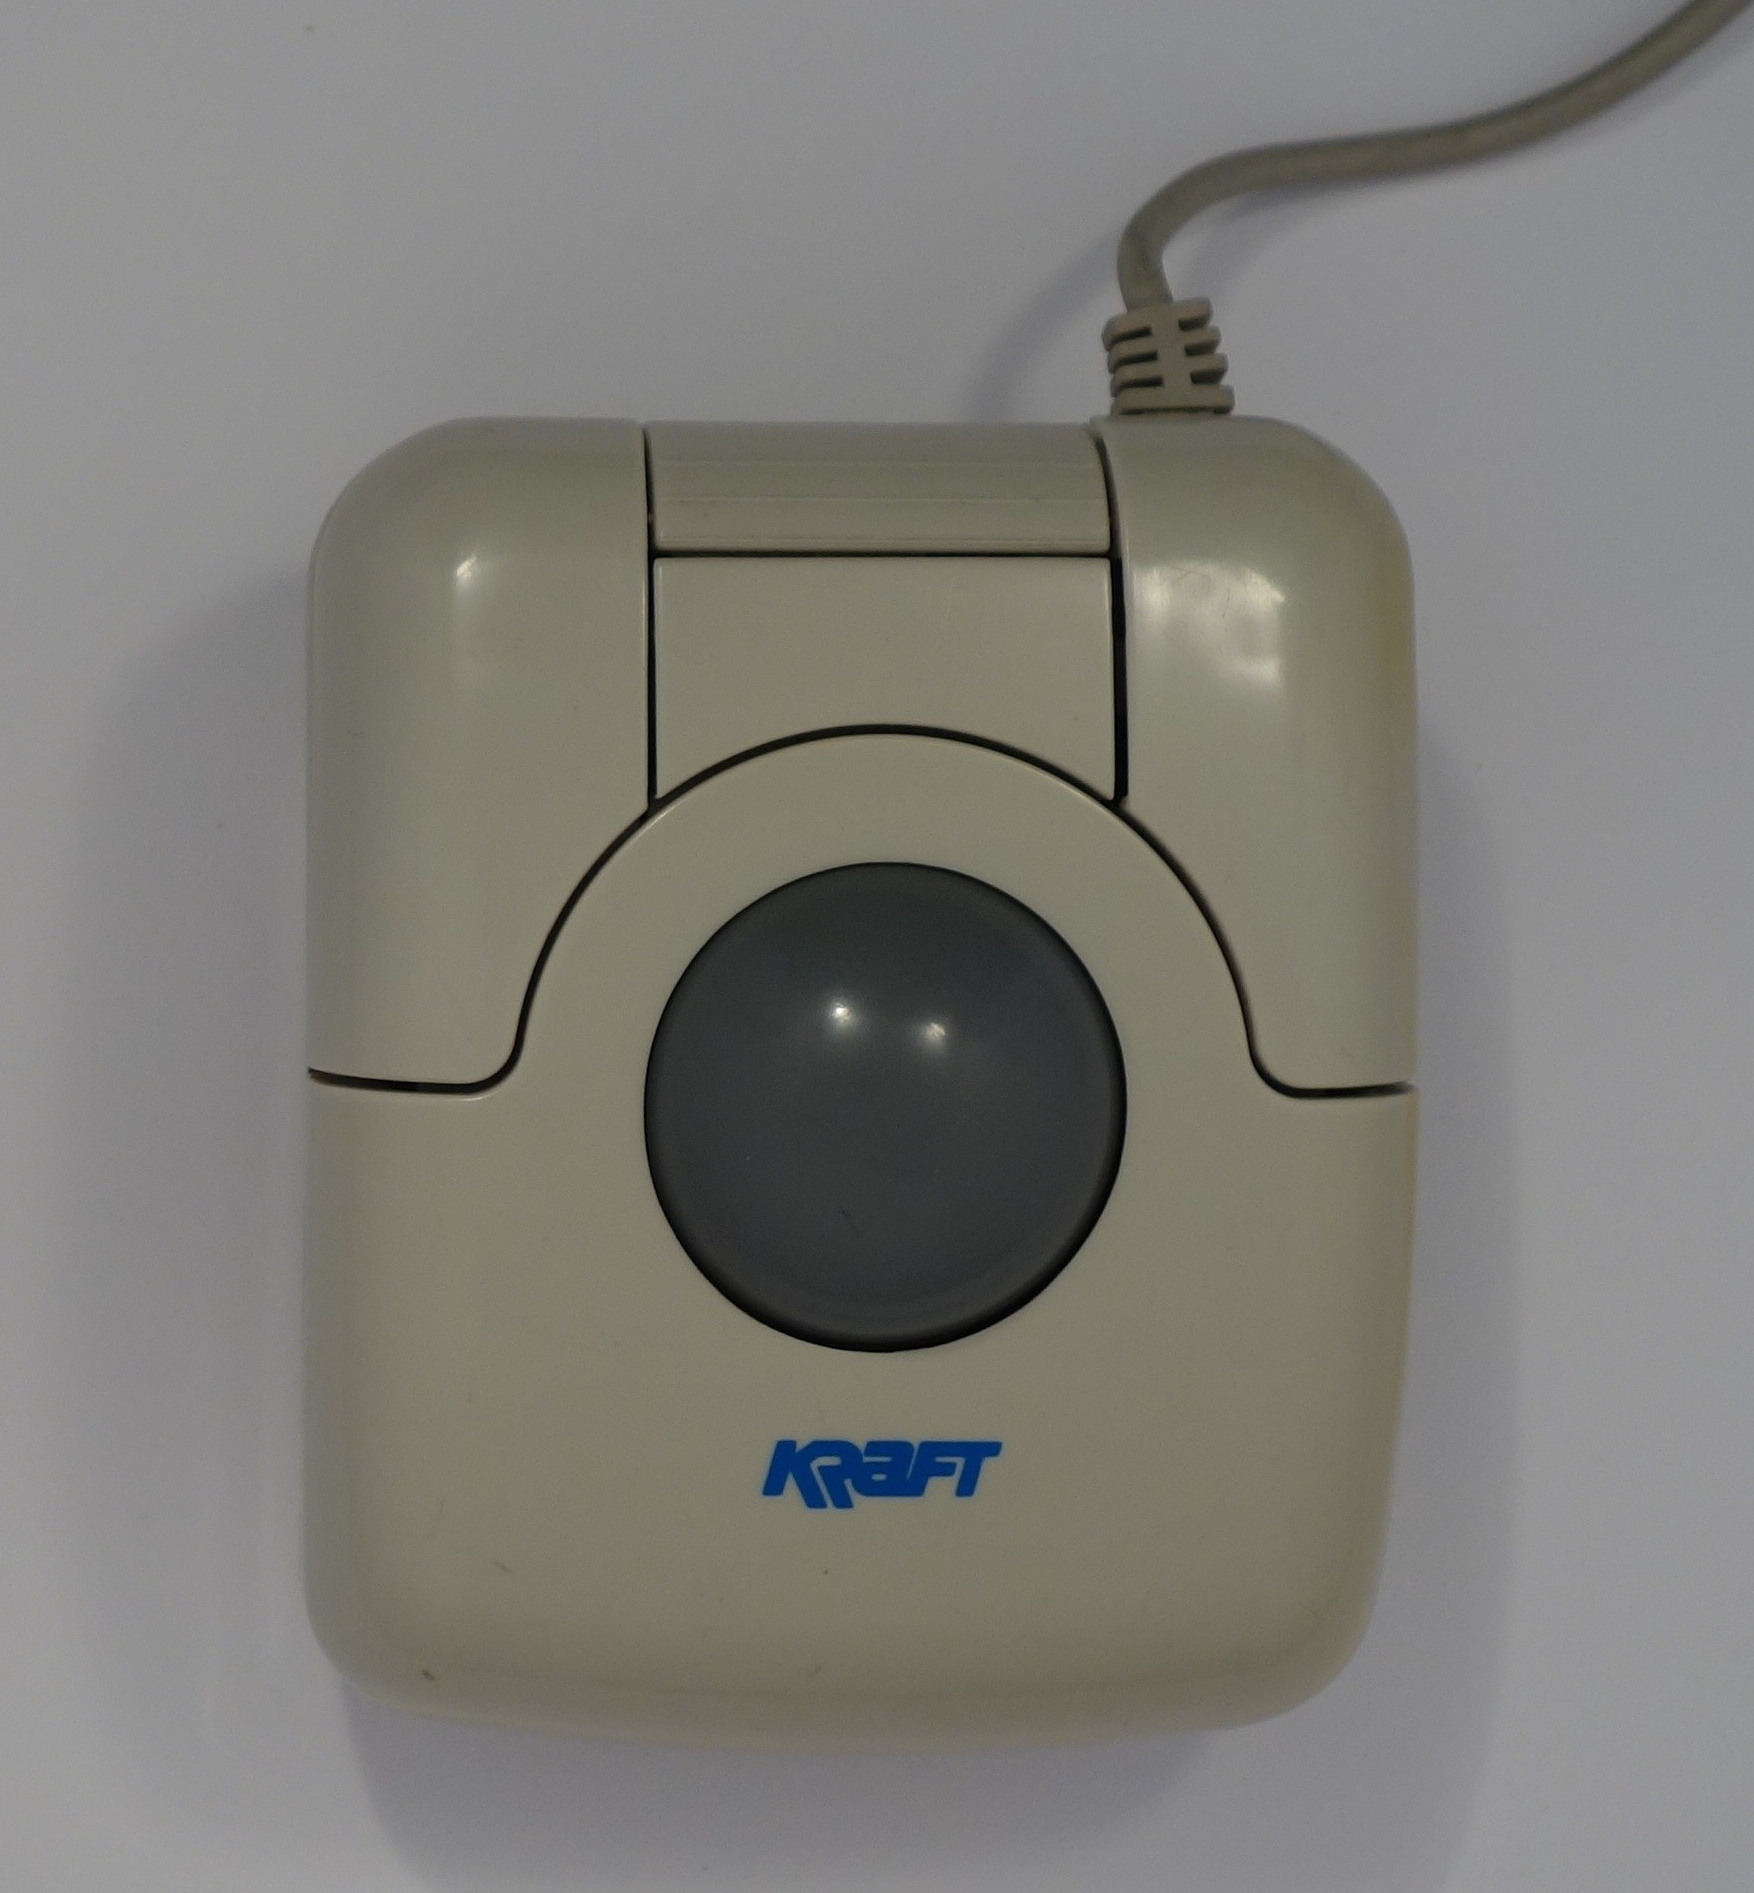
\includegraphics[scale=0.5]{1990_kraft_toptrack/2.9.jpg}
    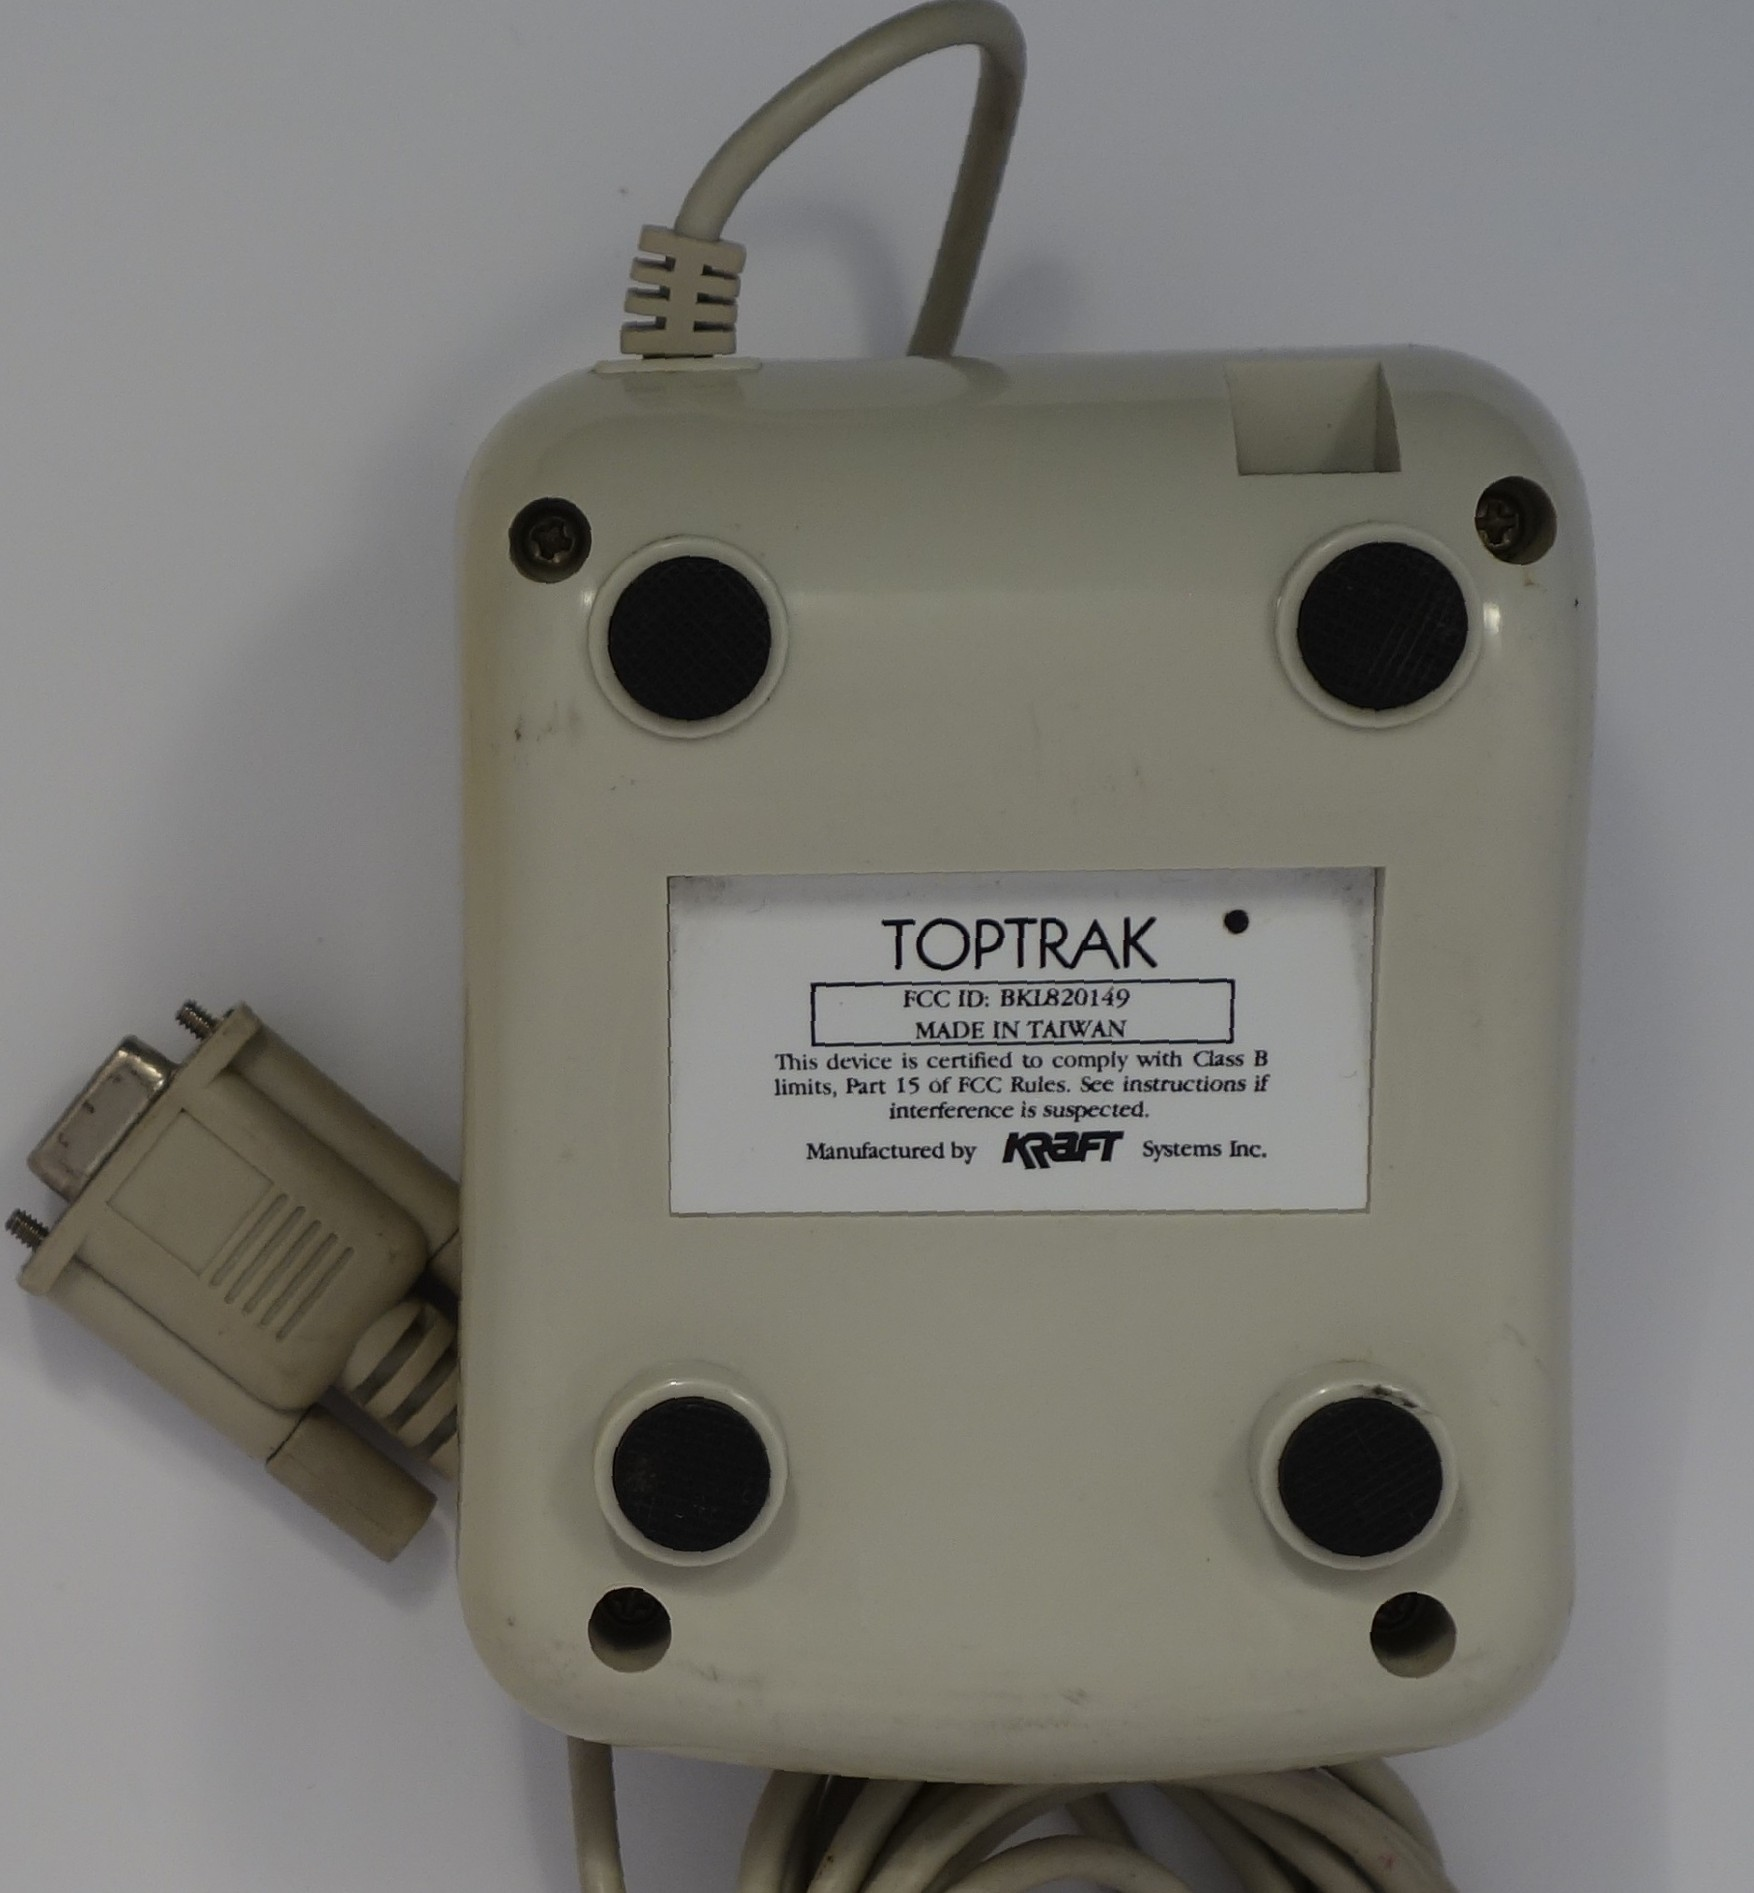
\includegraphics[scale=0.5]{1990_kraft_toptrack/2.10.jpg}
    \caption{TopTrak, вид сверху и снизу}
    \label{fig:TopTrakTopAndBottom}
\end{figure}

Дополнительно в комплекте с трекболом идёт стальная ножная педаль (рис. \ref{fig:TopTrakPedal}), которая служит альтернативой левой кнопке мыши, имеет еще один аналогичный кабель и добавляет дополнительные полкилограмма веса устройству.

\begin{figure}[h]
    \centering
    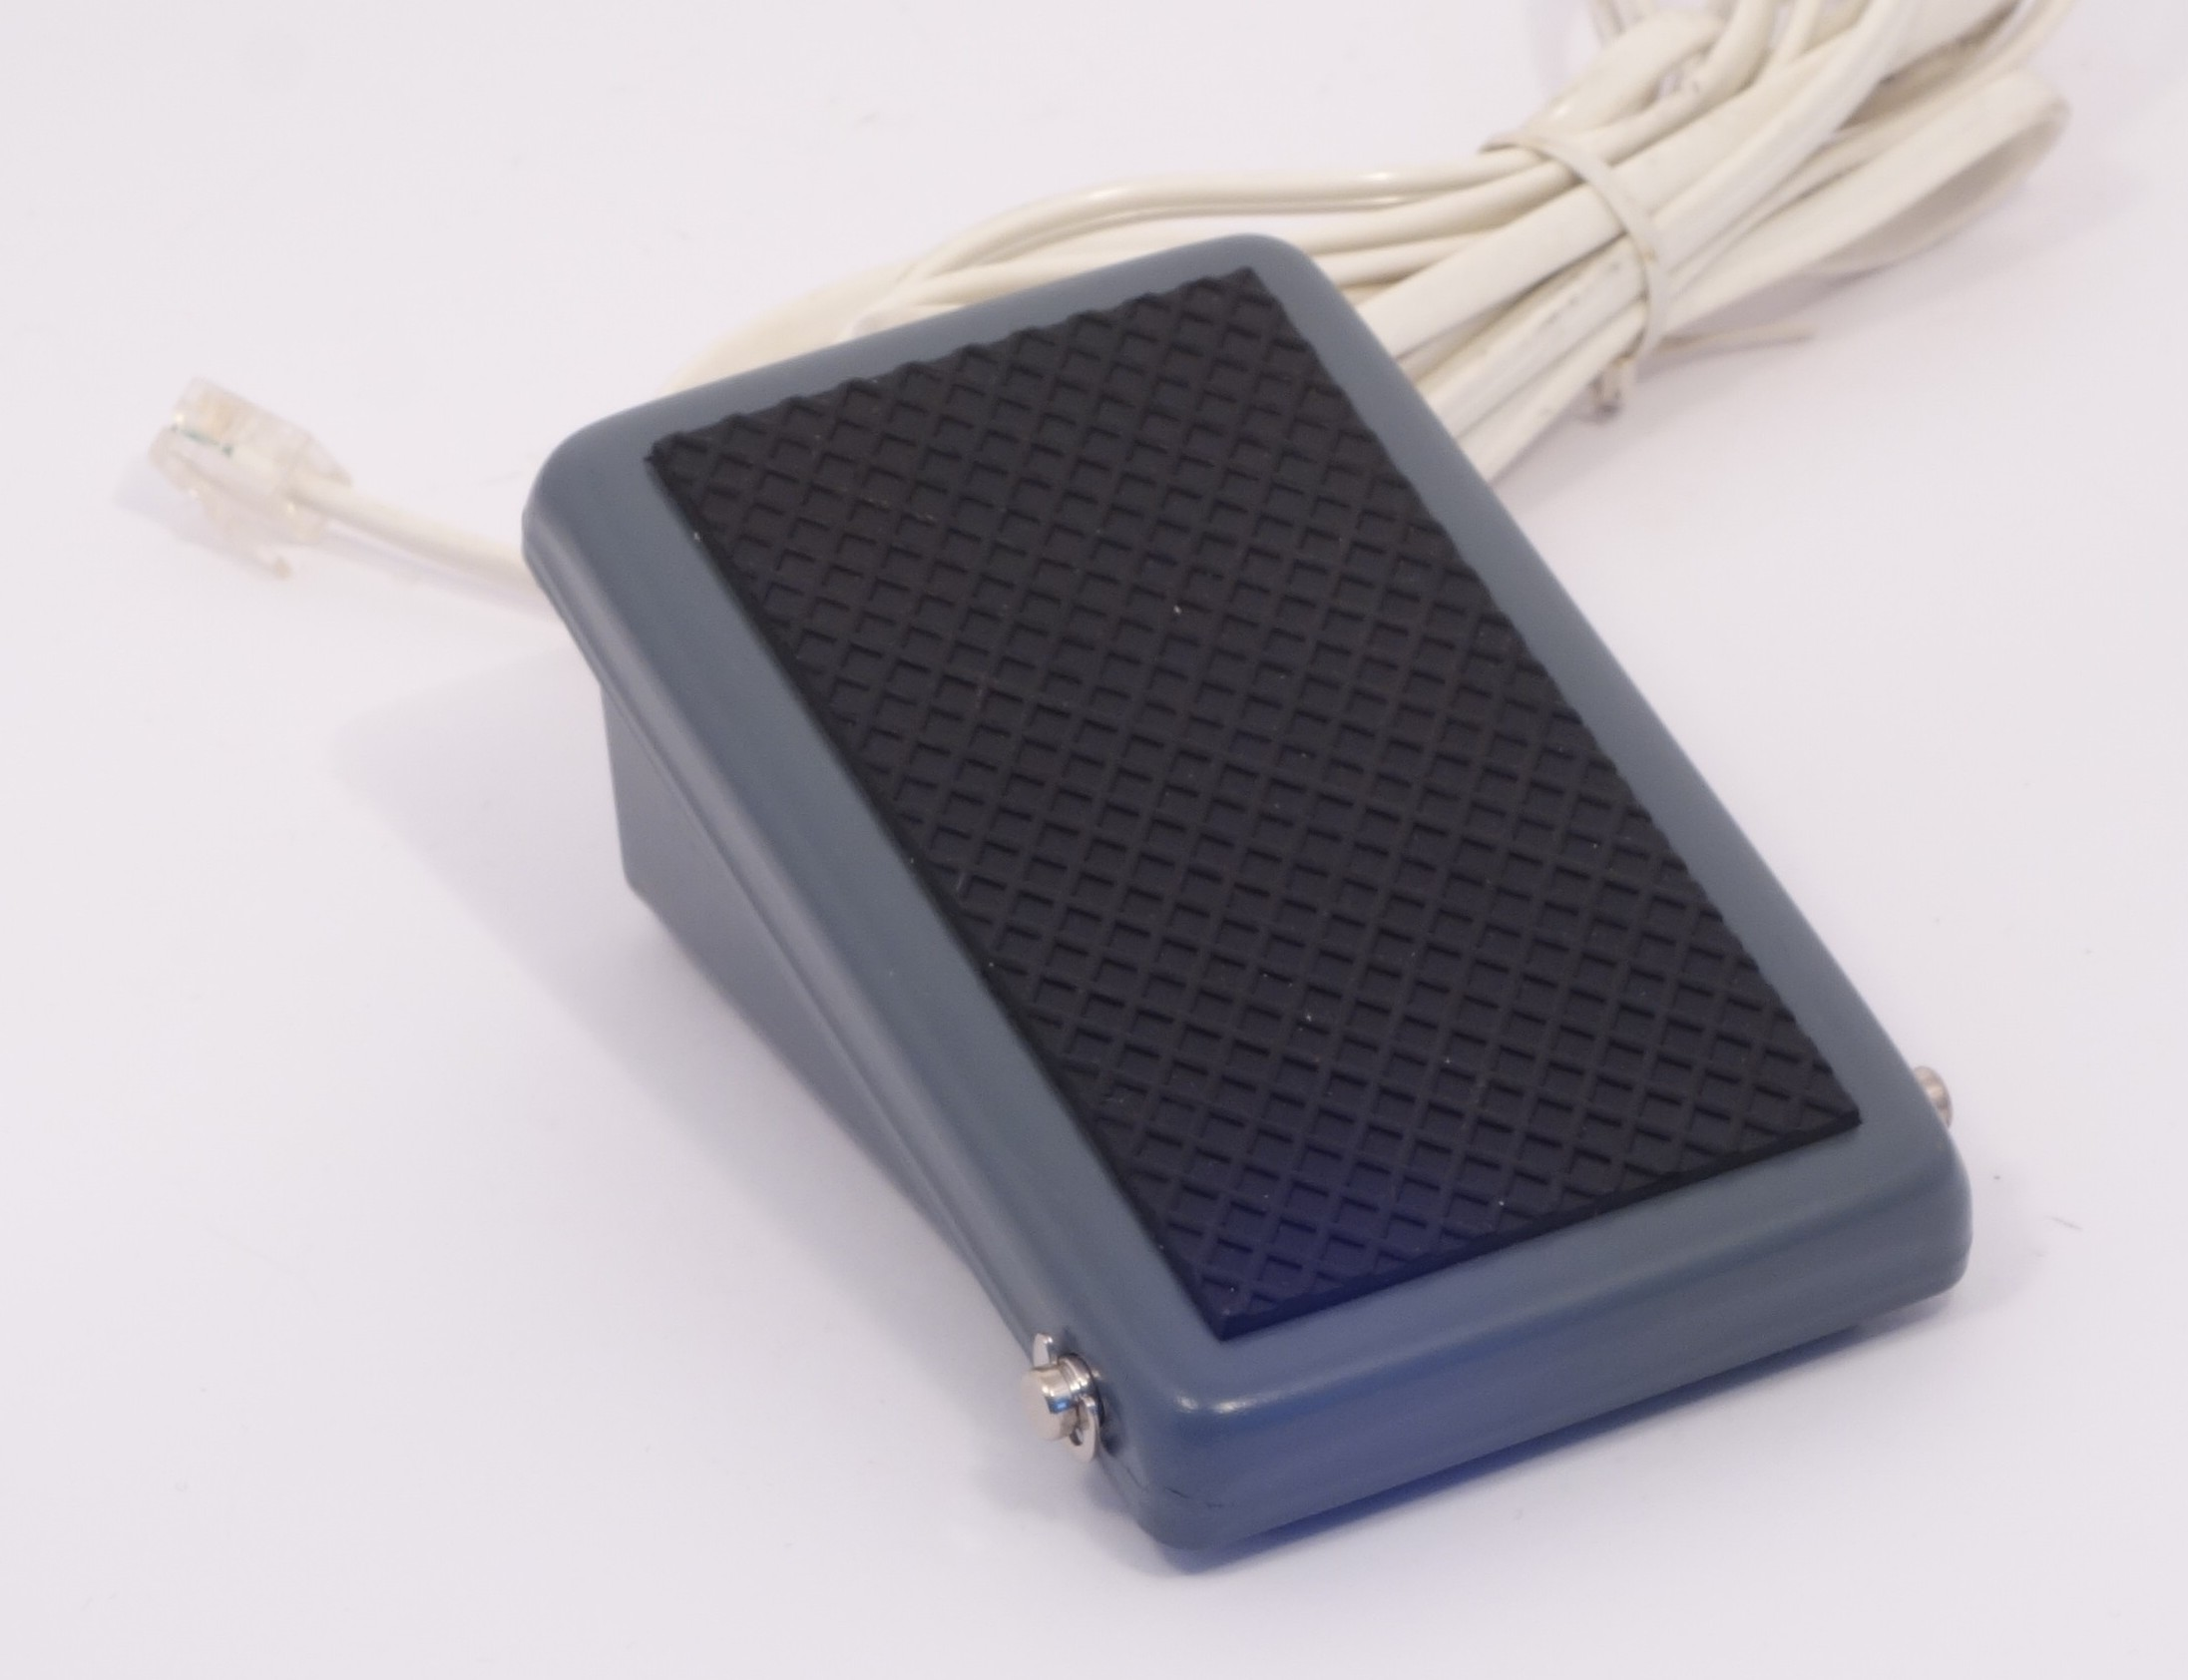
\includegraphics[scale=0.45]{1990_kraft_toptrack/2.7.jpg}
    \caption{Изображение педали для мыши TopTrak}
    \label{fig:TopTrakPedal}
\end{figure}

%\begin{figure}[h]
%    \centering
%    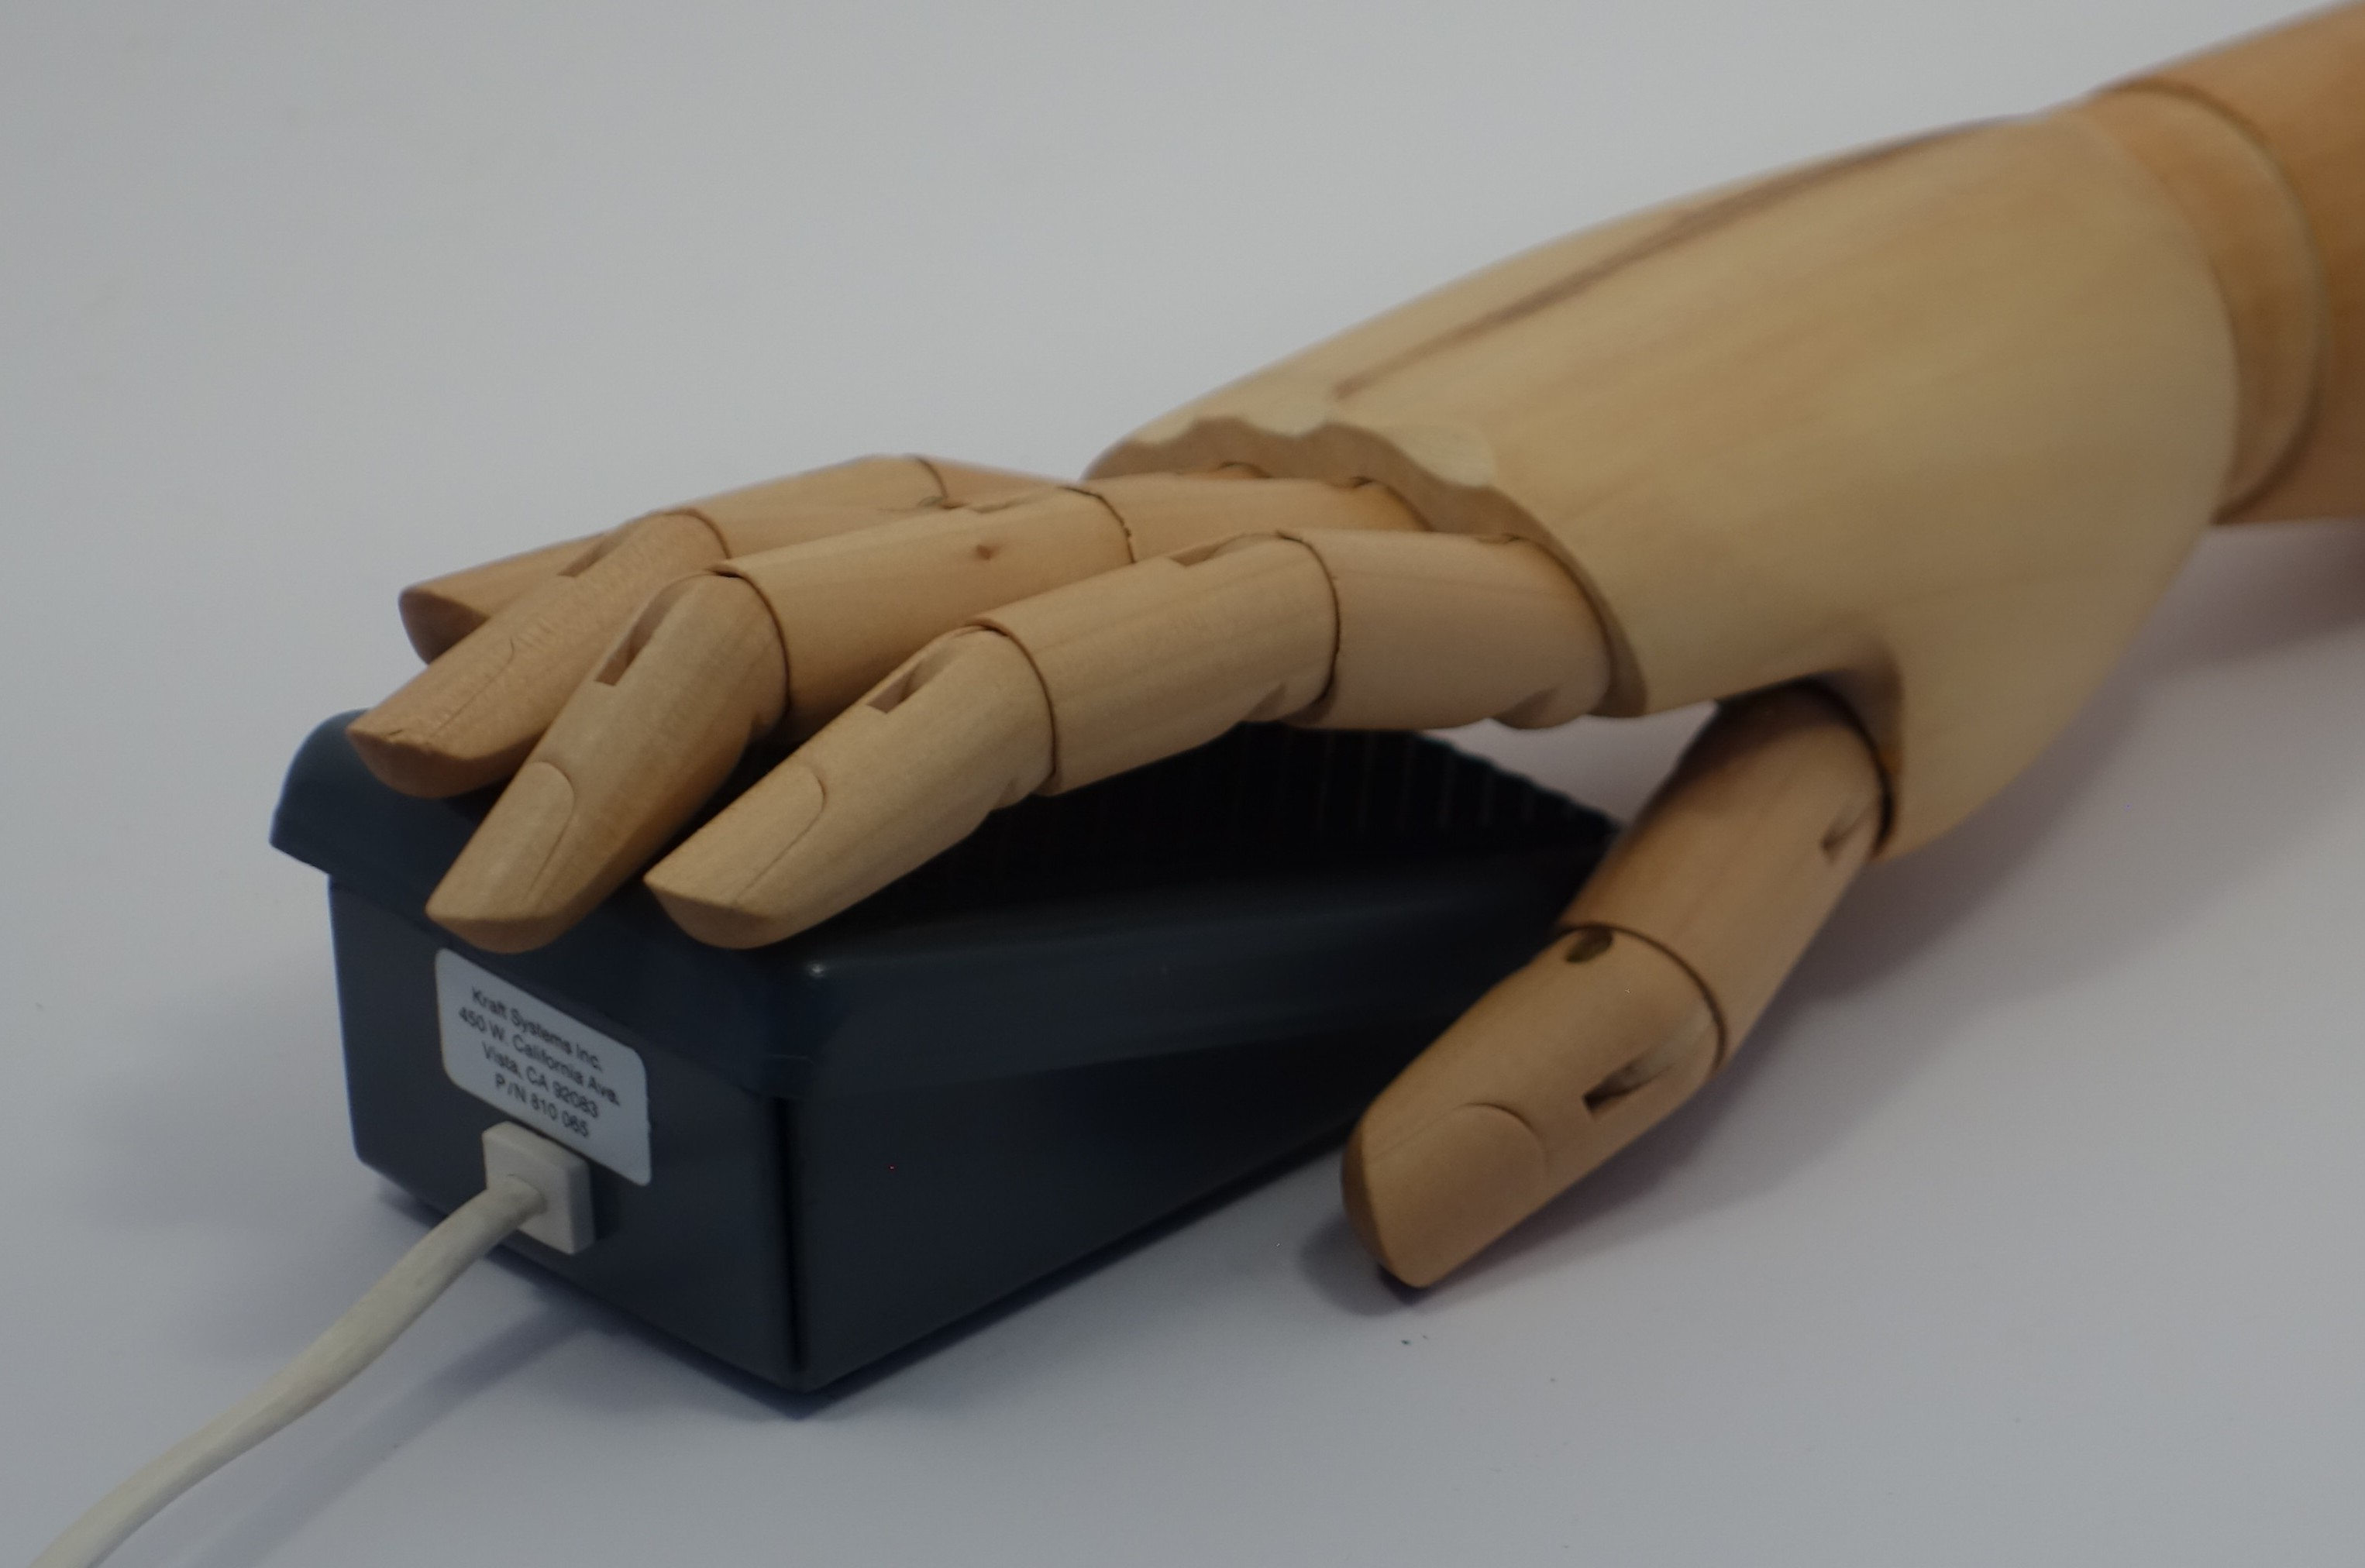
\includegraphics[scale=0.4]{1990_kraft_toptrack/2.8.jpg}
%    \caption{Изображение педали для мыши TopTrak с моделью руки человека}
%    \label{fig:TopTrakPedalHand}
%\end{figure}

Левая и правая кнопки TopTrak полностью занимают верхние углы.

\begin{figure}[h]
    \centering
    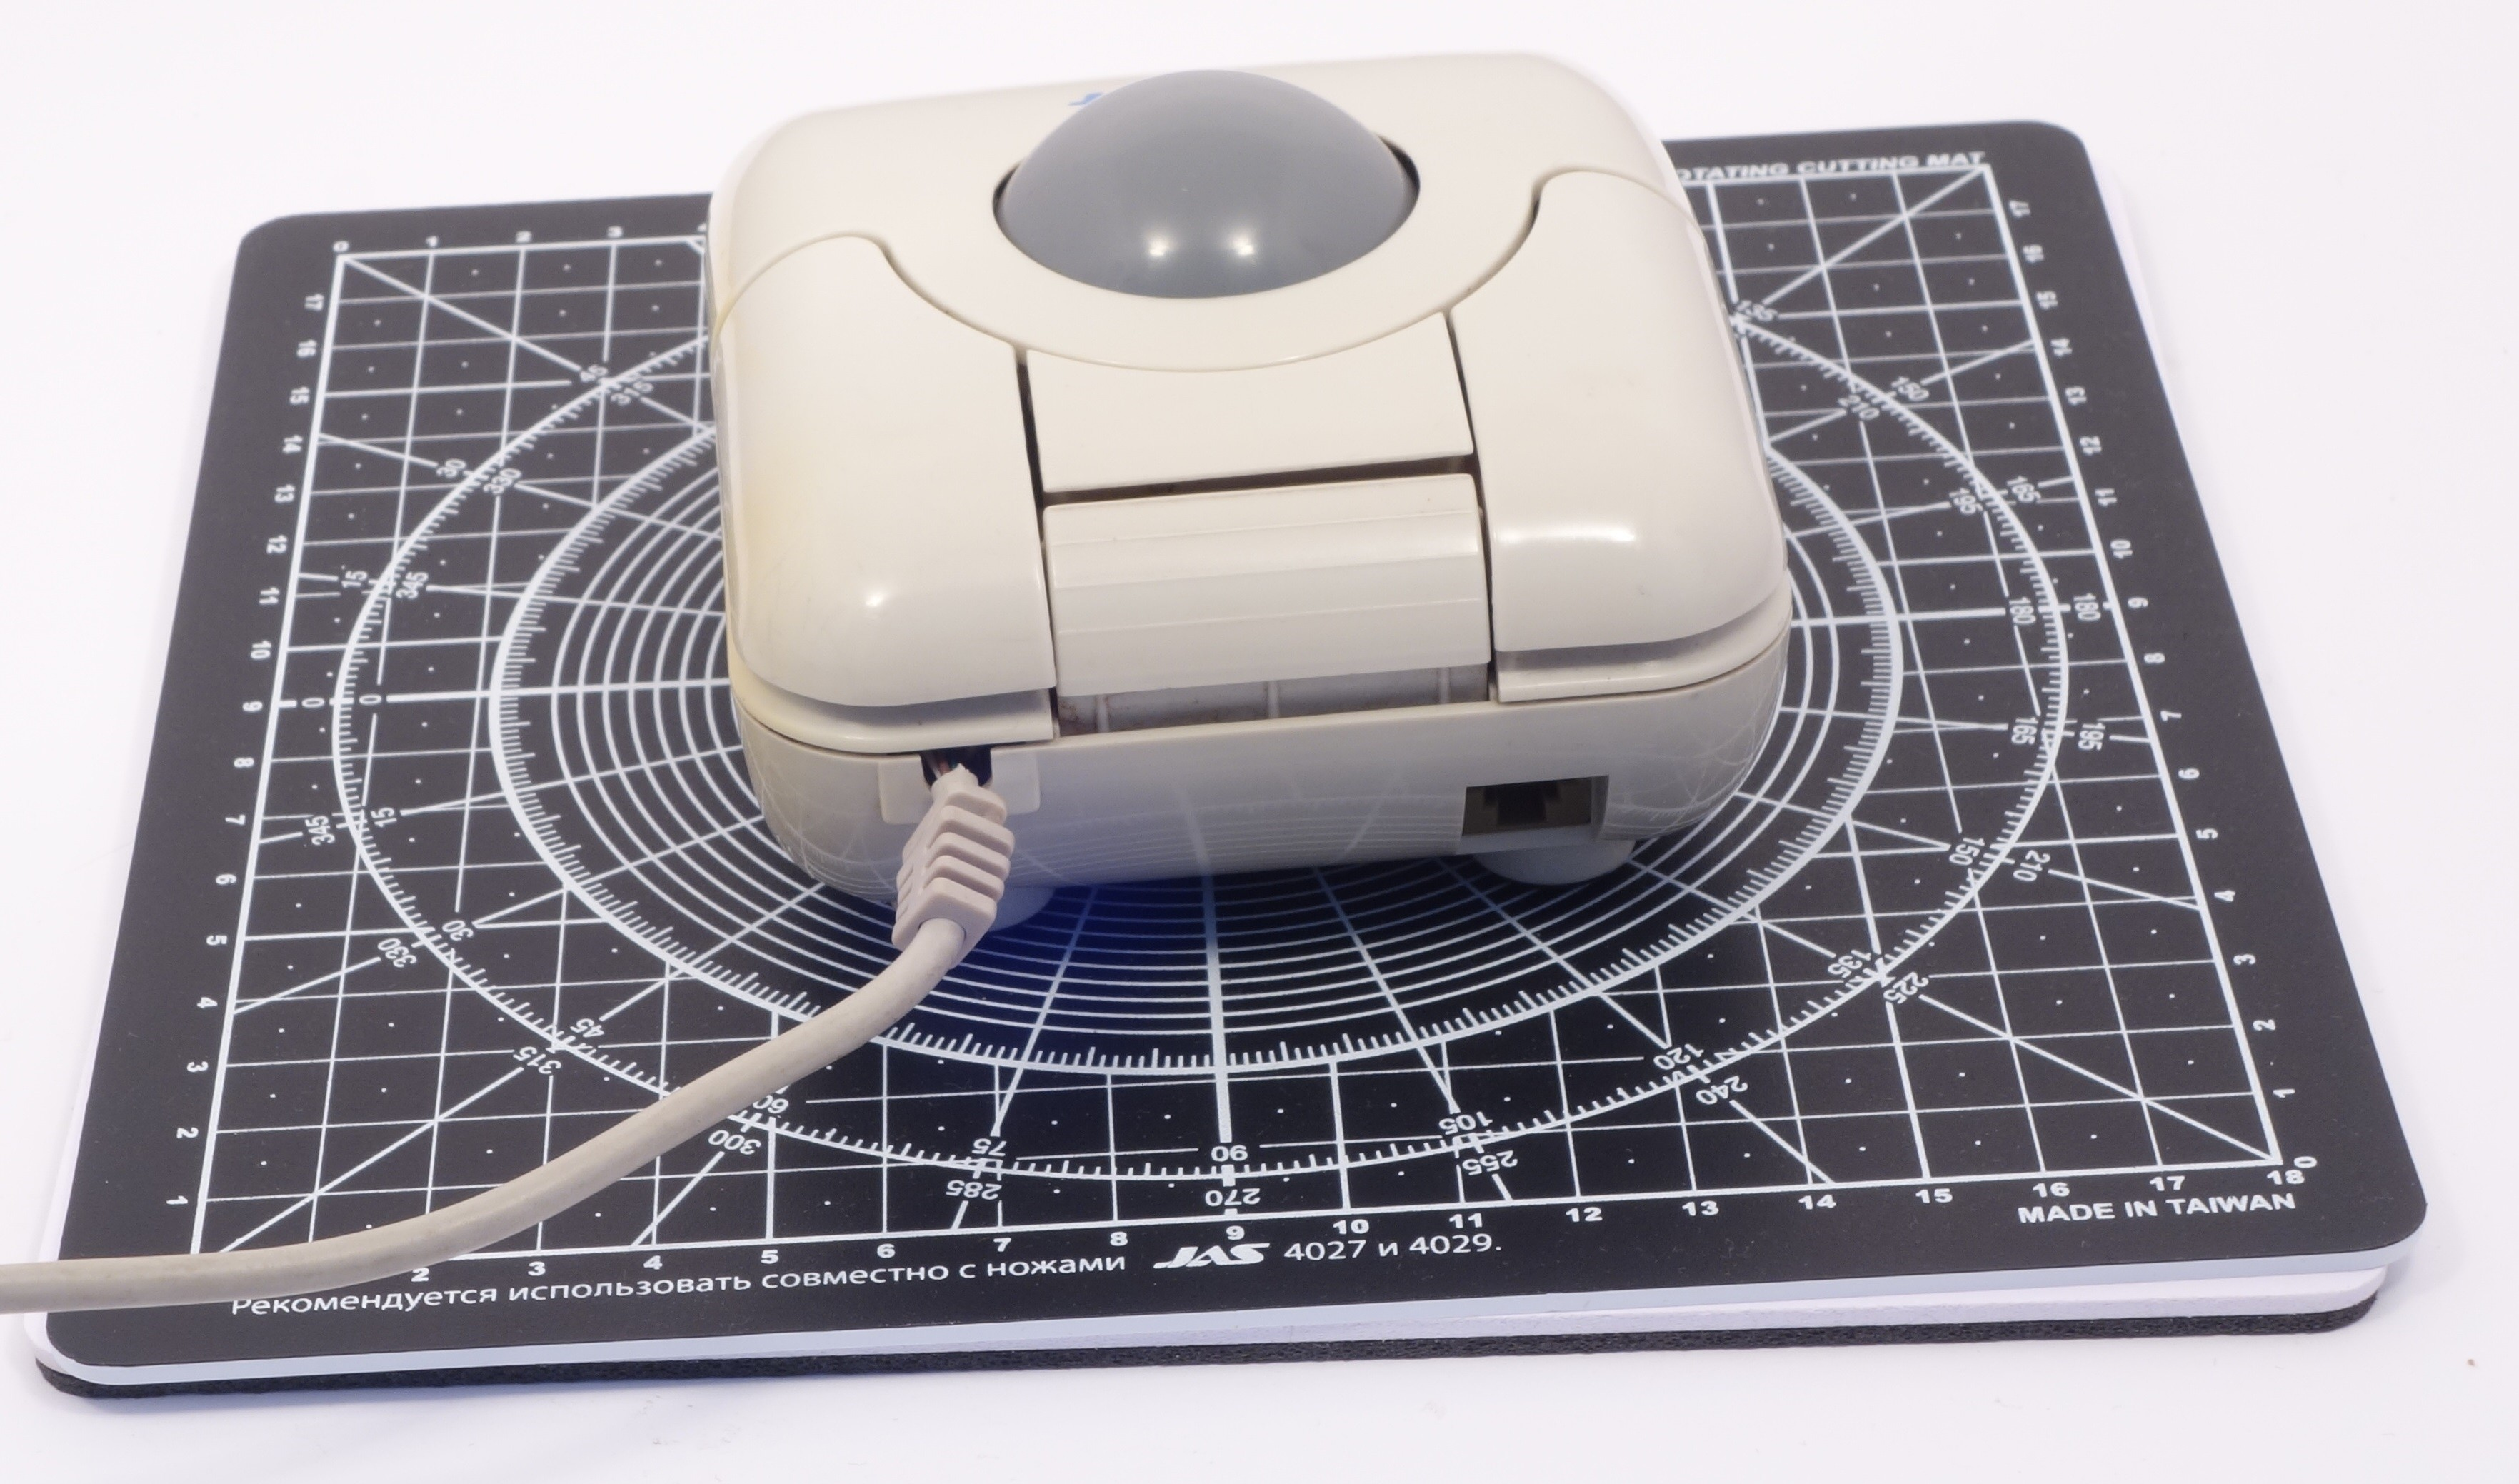
\includegraphics[scale=0.35]{1990_kraft_toptrack/2.6.jpg}
    \caption{Изображение TopTrak на размерном коврике с шагом сетки 1~см}
    \label{fig:TopTrakSize}
\end{figure}


TopTrak может быть подходящим устройством для настольного компьютера, но он слишком громоздкий, чтобы его всерьез рассматривать для портативных компьютеров.

\begin{figure}[h]
    \centering
    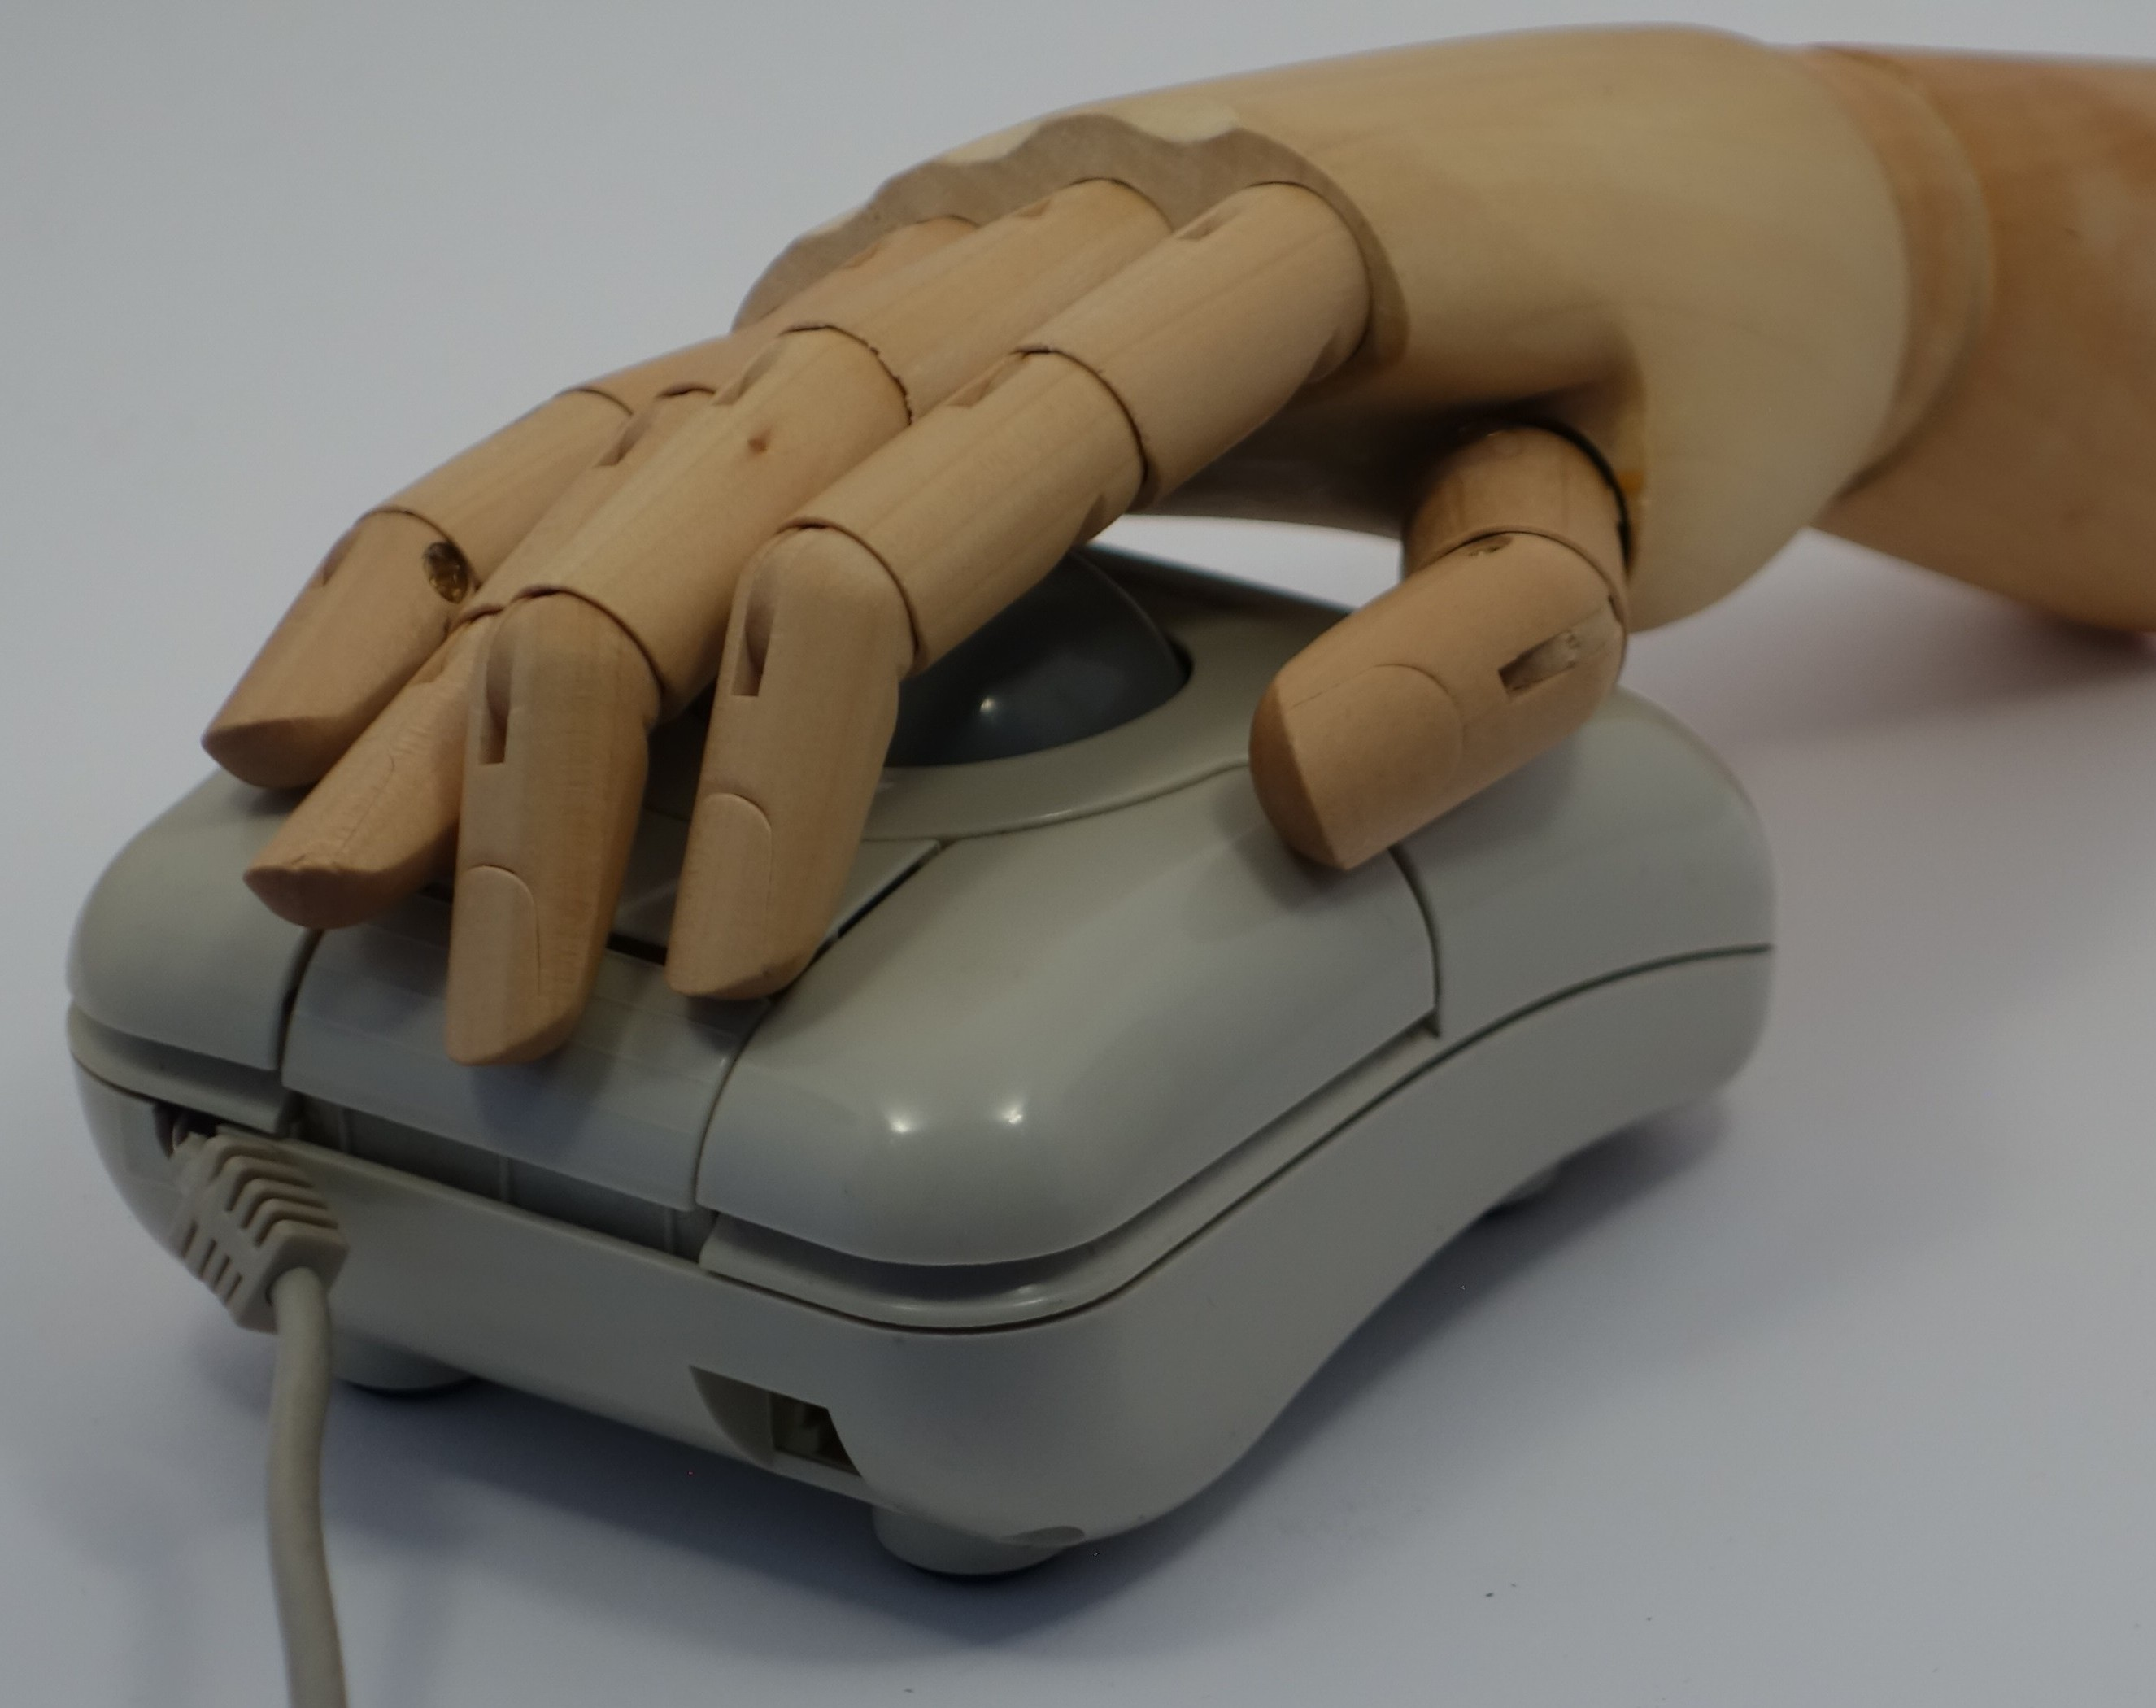
\includegraphics[scale=0.45]{1990_kraft_toptrack/2.5.jpg}
    \caption{Изображение TopTrak с моделью руки человека}
    \label{fig:TopTrakHand}
\end{figure}

Как можно видеть, маркировка TopTrak содержит код FCC ID (рис. \ref{fig:TopTrakTopAndBottom}). Проверка кода по базе данных Федеральной комиссии по коммуникациям США показывает, что трекбол был разработан американской компанией Kraft Systems в 1990 году.

%\begin{figure}[htpb]
%    \centering
%    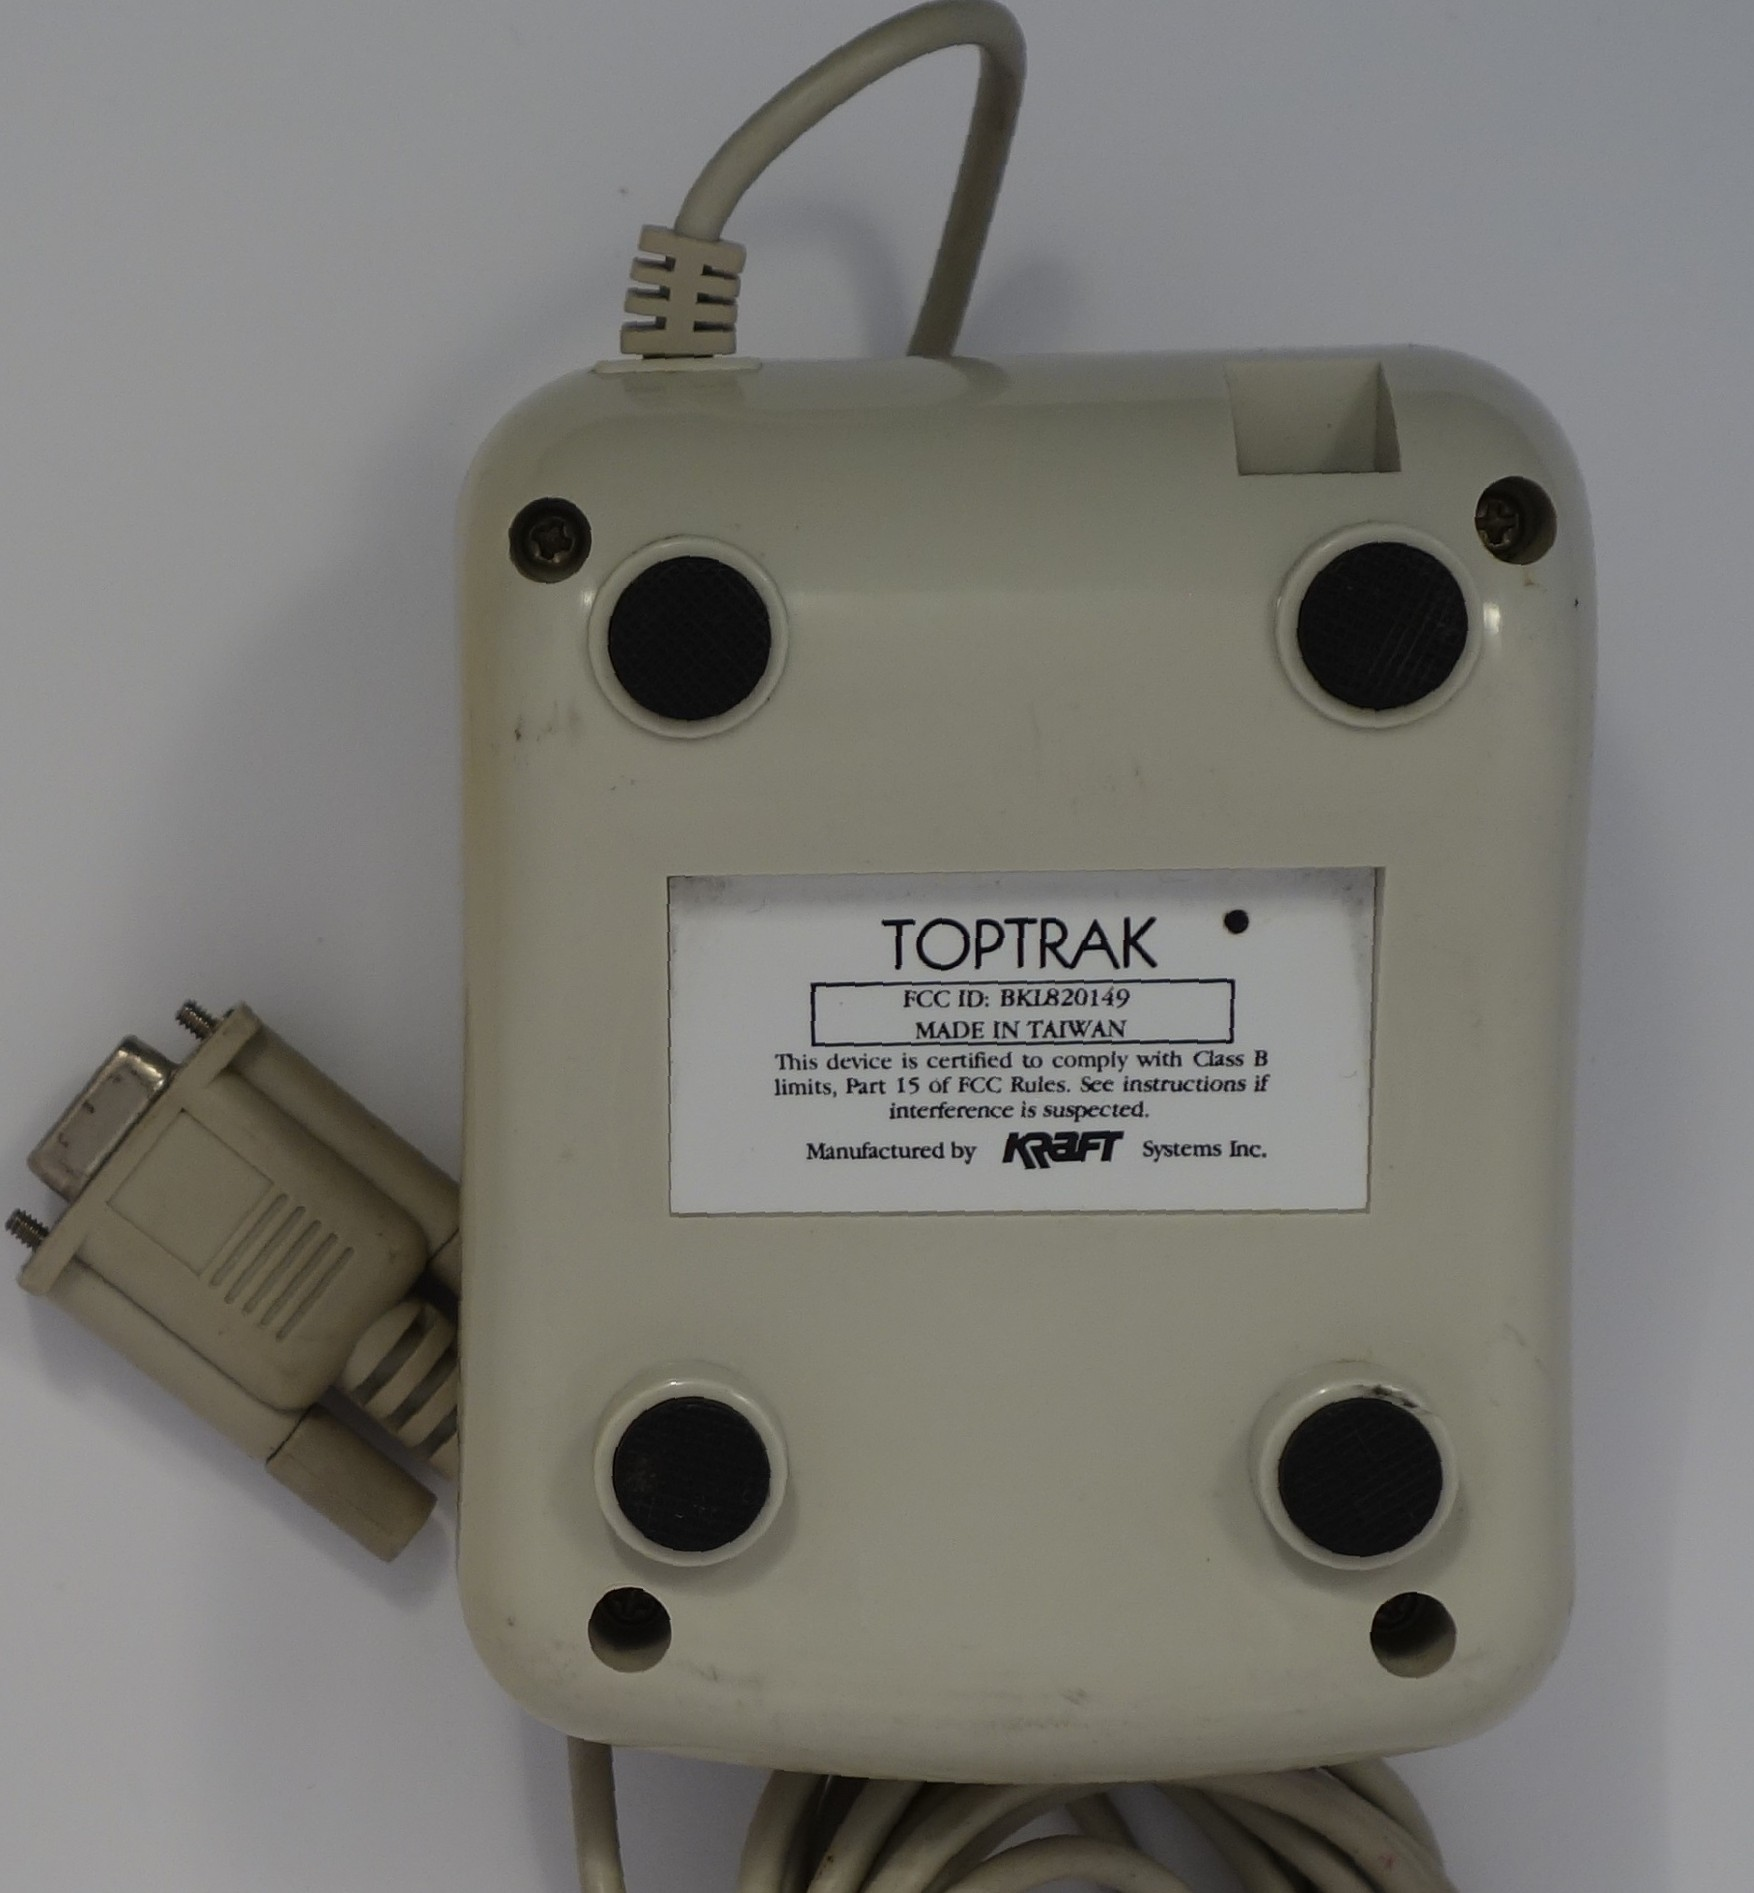
\includegraphics[scale=0.4]{1990_kraft_toptrack/2.10.jpg}
%    \caption{TopTrak, вид снизу}
%    \label{fig:TopTrakBottom}
%\end{figure}

Изучение разобранного трекбола (рис. \ref{fig:TopTrakInside}) показывает, что он выполнен по стандартной оптомеханической схеме, а массивные металлические ролики с подшипниками качения показывают, что трекбол был задуман как достаточно долговечное устройство, не относящееся к нижнему ценовому диапазону.

\begin{figure}[h]
    \centering
    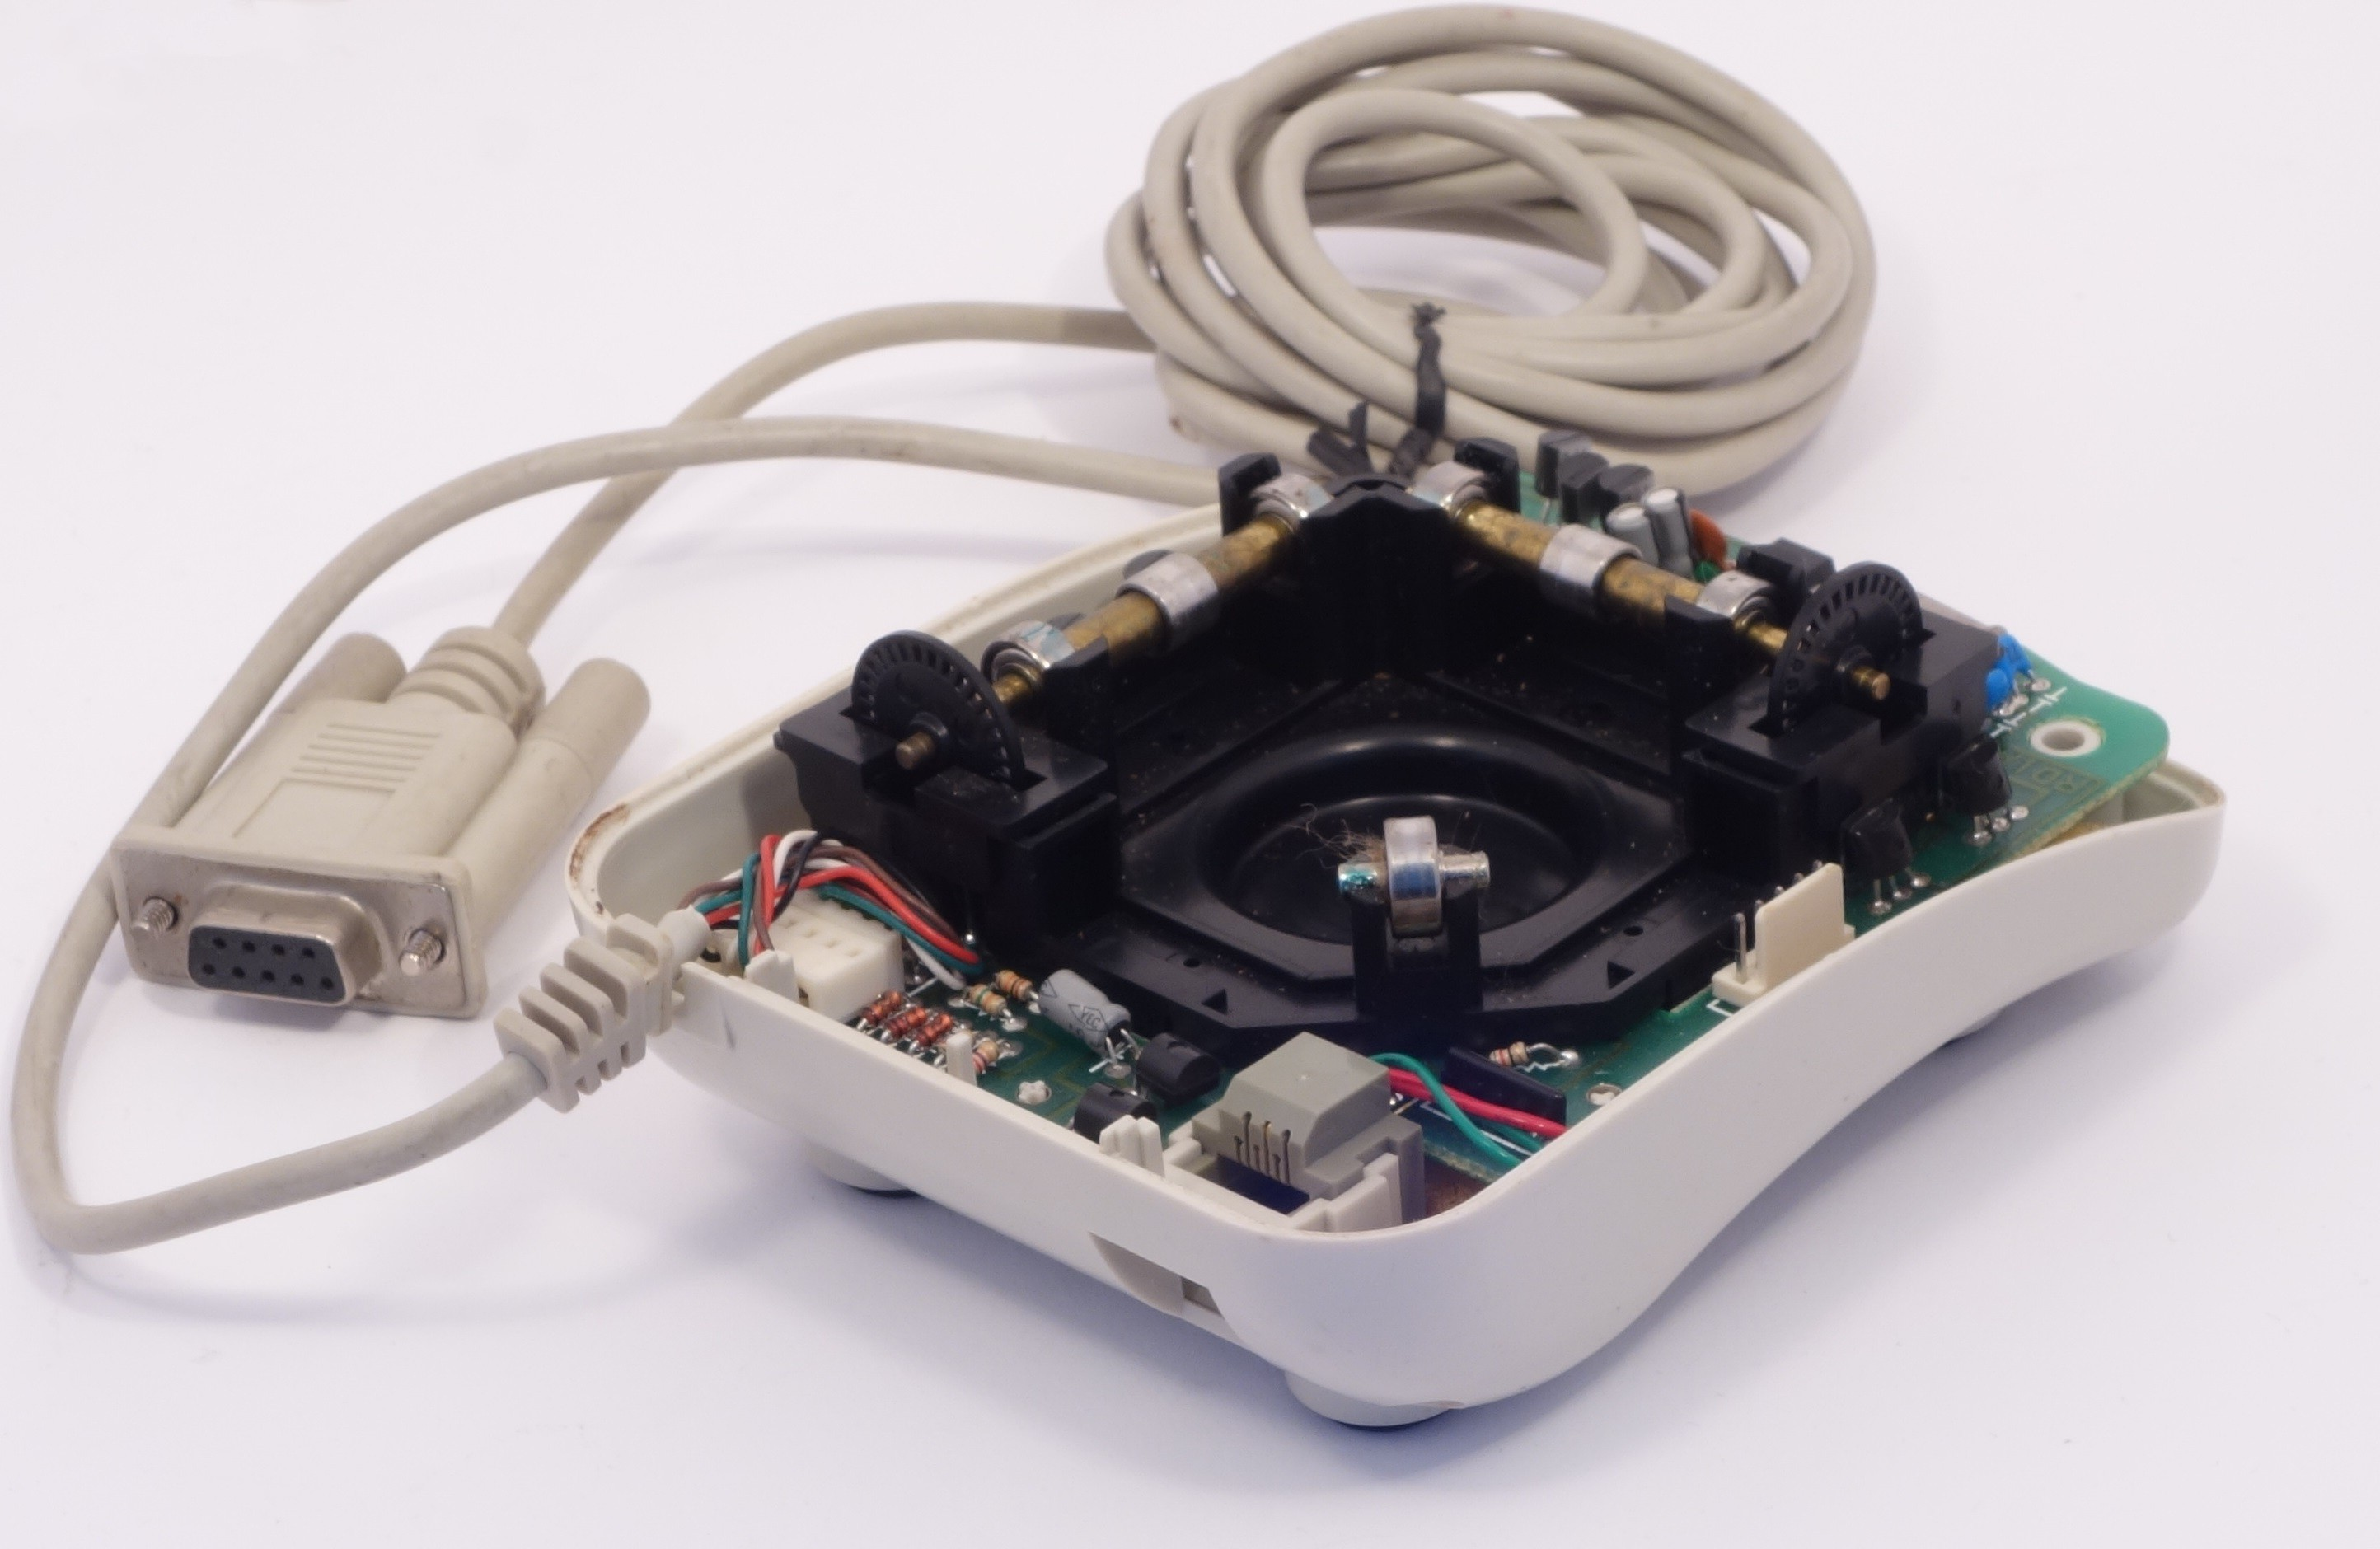
\includegraphics[scale=0.5]{1990_kraft_toptrack/200.jpg}
    \caption{TopTrak изнутри}
    \label{fig:TopTrakInside}
\end{figure}

\begin{thebibliography}{9}
\bibitem {mouses} Berlin E. TopTrak // PC Magazine. October 15, 1991. p. 126-127
\end{thebibliography}
\end{document}

\documentclass[11pt, a4paper]{article}
\usepackage{pdfpages}
\usepackage{parallel}
\usepackage[T2A]{fontenc}
\usepackage{ucs}
\usepackage[utf8x]{inputenc}
\usepackage[polish,english,russian]{babel}
\usepackage{hyperref}
\usepackage{rotating}
\usepackage[inner=2cm,top=1.8cm,outer=2cm,bottom=2.3cm,nohead]{geometry}
\usepackage{listings}
\usepackage{graphicx}
\usepackage{wrapfig}
\usepackage{longtable}
\usepackage{indentfirst}
\usepackage{array}
\usepackage{tikzsymbols}
\usepackage{soul}
\usepackage[ruled,vlined]{algorithm2e}
%\counterwithout{figure}{section} 

\usepackage{url}
\makeatletter
\g@addto@macro{\UrlBreaks}{\UrlOrds}
\makeatother

\newcolumntype{P}[1]{>{\raggedright\arraybackslash}p{#1}}
\frenchspacing
\usepackage{fixltx2e} %text sub- and superscripts
\usepackage{icomma} % коскі ў матэматычным рэжыме
\PreloadUnicodePage{4}

\newcommand{\longpage}{\enlargethispage{\baselineskip}}
\newcommand{\shortpage}{\enlargethispage{-\baselineskip}}

\def\switchlang#1{\expandafter\csname switchlang#1\endcsname}
\def\switchlangbe{
\let\saverefname=\refname%
\def\refname{Літаратура}%
\def\figurename{Іл.}%
}
\def\switchlangen{
\let\saverefname=\refname%
\def\refname{References}%
\def\figurename{Fig.}%
}
\def\switchlangru{
\let\saverefname=\refname%
\let\savefigurename=\figurename%
\def\refname{Литература}%
\def\figurename{Рис.}%
}

\hyphenation{admi-ni-stra-tive}
\hyphenation{ex-pe-ri-ence}
\hyphenation{fle-xi-bi-li-ty}
\hyphenation{Py-thon}
\hyphenation{ma-the-ma-ti-cal}
\hyphenation{re-ported}
\hyphenation{imp-le-menta-tions}
\hyphenation{pro-vides}
\hyphenation{en-gi-neering}
\hyphenation{com-pa-ti-bi-li-ty}
\hyphenation{im-pos-sible}
\hyphenation{desk-top}
\hyphenation{elec-tro-nic}
\hyphenation{com-pa-ny}
\hyphenation{de-ve-lop-ment}
\hyphenation{de-ve-loping}
\hyphenation{de-ve-lop}
\hyphenation{da-ta-ba-se}
\hyphenation{plat-forms}
\hyphenation{or-ga-ni-za-tion}
\hyphenation{pro-gramming}
\hyphenation{in-stru-ments}
\hyphenation{Li-nux}
\hyphenation{sour-ce}
\hyphenation{en-vi-ron-ment}
\hyphenation{Te-le-pathy}
\hyphenation{Li-nux-ov-ka}
\hyphenation{Open-BSD}
\hyphenation{Free-BSD}
\hyphenation{men-ti-on-ed}
\hyphenation{app-li-ca-tion}

\def\progref!#1!{\texttt{#1}}
\renewcommand{\arraystretch}{2} %Іначай формулы ў матрыцы зліпаюцца з лініямі
\usepackage{array}

\def\interview #1 (#2), #3, #4, #5\par{

\section[#1, #3, #4]{#1 -- #3, #4}
\def\qname{LVEE}
\def\aname{#1}
\def\q ##1\par{{\noindent \bf \qname: ##1 }\par}
\def\a{{\noindent \bf \aname: } \def\qname{L}\def\aname{#2}}
}

\def\interview* #1 (#2), #3, #4, #5\par{

\section*{#1\\{\small\rm #3, #4. #5}}
\ifx\ParallelWhichBox\undefined%
    \addcontentsline{toc}{section}{#1, #3, #4}%
\else%
\ifnum\ParallelWhichBox=0%
    \addcontentsline{toc}{section}{#1, #3, #4}%
\fi\fi%

\def\qname{LVEE}
\def\aname{#1}
\def\q ##1\par{{\noindent \bf \qname: ##1 }\par}
\def\a{{\noindent \bf \aname: } \def\qname{L}\def\aname{#2}}
}

\newcommand{\interviewfooter}[1]{
\vskip 1em
\noindent \textit{#1}
}


\begin{document}

\title{1991 "--- MicroSpeed PC-TRACK trackball}
\date{}
\maketitle
Трекбол PC-TRACK от MicroSpeed, выпущенный в 1991 году, имеет существенно более продуманный эргономичный дизайн, чем предыдущая модель этой фирмы, трекбол FastTRAP.

\begin{figure}[h]
    \centering
    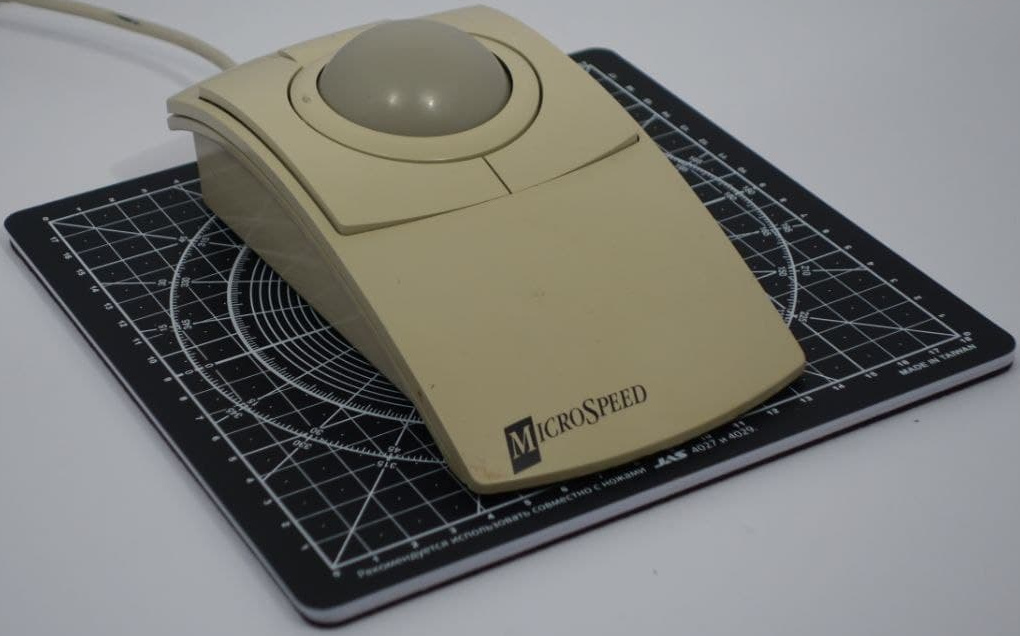
\includegraphics[scale=0.3]{1991_microspeed_pc-track/PC.jpg}
    \caption{Изображение PC-TRACK на размерном коврике с шагом сетки 1 см}
    \label{fig:PCTRACKSize}
\end{figure}

Шар трекбола окружен по бокам крупными выпуклыми кнопками, и дополнительно за шаром расположена третья кнопка меньшего размера. Такое расположение основных кнопок является для трекбола близким к оптимальному; поскольку левая и правая кнопки имеют большую длину, пользователь может перемещать шар ладонью или подушечками пальцев, а большой палец и мизинец использовать для нажатия на кнопки. Кроме того, этот вариант является симметричным, поэтому одинаково хорошо подходит как для правшей, так и для левшей \ref{fig:PCTRACKHand}. Выпуклая форма PC-TRAC спроектирована таким образом, чтобы соответствовать естественному изгибу руки. Ближняя к пользователю часть корпуса фактически сливается с поверхностью стола, так что, по словам производителя, устранена присутствовашая в более ранних конструкциях ступенька, создававшая нагрузку на запястье. Уменьшая угол наклона запястья и руки, Micro Speed сводит к минимуму усталость и в то же время позволяет сохранять точность и контроль.

\begin{figure}[h]
    \centering
    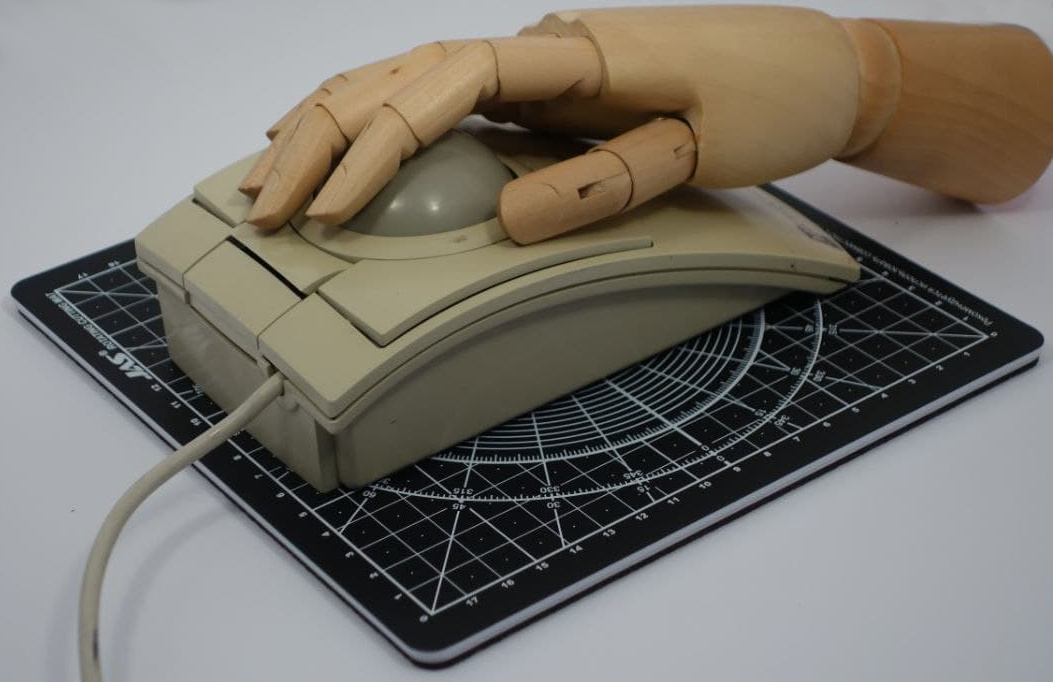
\includegraphics[scale=0.3]{1991_microspeed_pc-track/PC1.jpg}
    \caption{Изображение PC-TRACK с моделью руки человека}
    \label{fig:PCTRACKHand}
\end{figure}

Меньшая по размеру третья кнопка может использоваться как средняя кнопка мыши или действовать как блокировка перетаскивания. Одна из основных проблем при использовании трекболов с графическими интерфейсами, такими как Windows, на рубеже 80-х и 90-х годов виделась в том, что пользователю сложно перемещать указатель, удерживая нажатой кнопку. Если включена функция блокировки перетаскивания, можно нажать среднюю кнопку после того, как указатель спозиционирован на начальной позиции, переместить указатель к конечной позиции и снова нажать среднюю кнопку, чтобы закончить перетаскивание объекта (с точки зрения компьютера, пользователь все это время удерживал кнопку нажатой). В дополнение к этой функции PC-TRAC также имеет аккордный режим, который позволяет имитировать удерживание обеих кнопок при перемещении мыши.

MicroSpeed выбрала для данного устройства 2,25-дюймовый шар, потому что их исследования показали значительное увеличение точности позиционирования курсора шаром большего диаметра. Исследования также показали, что лучшей точности также способствует больший вес шара; поэтому примененный в этом трекболе 2,25-дюймовый шар обладает на 30 процентов большим весом, чем 2-дюймовый шар, и на 70 процентов большим, чем 1,5-дюймовый шар.

С точки зрения программного обеспечения трекбол полностью совместим с драйвером мыши Microsoft. Включенные в комплект поставки драйверы PrecisionPointer для DOS и Windows предлагают ряд улучшений, специфичных для трекбола, таких как ускорение при движении курсора (расстояние, на которое перемещается указатель, зависит от того, как быстро вы вращаете шар). Также в комплект входит утилита переназначения клавиш, драйвер для консольных приложений, имитирующий срабатывание курсорных клавиш при вращении шара, а также драйвер для игры в Тетрис.

\begin{figure}[h]
    \centering
    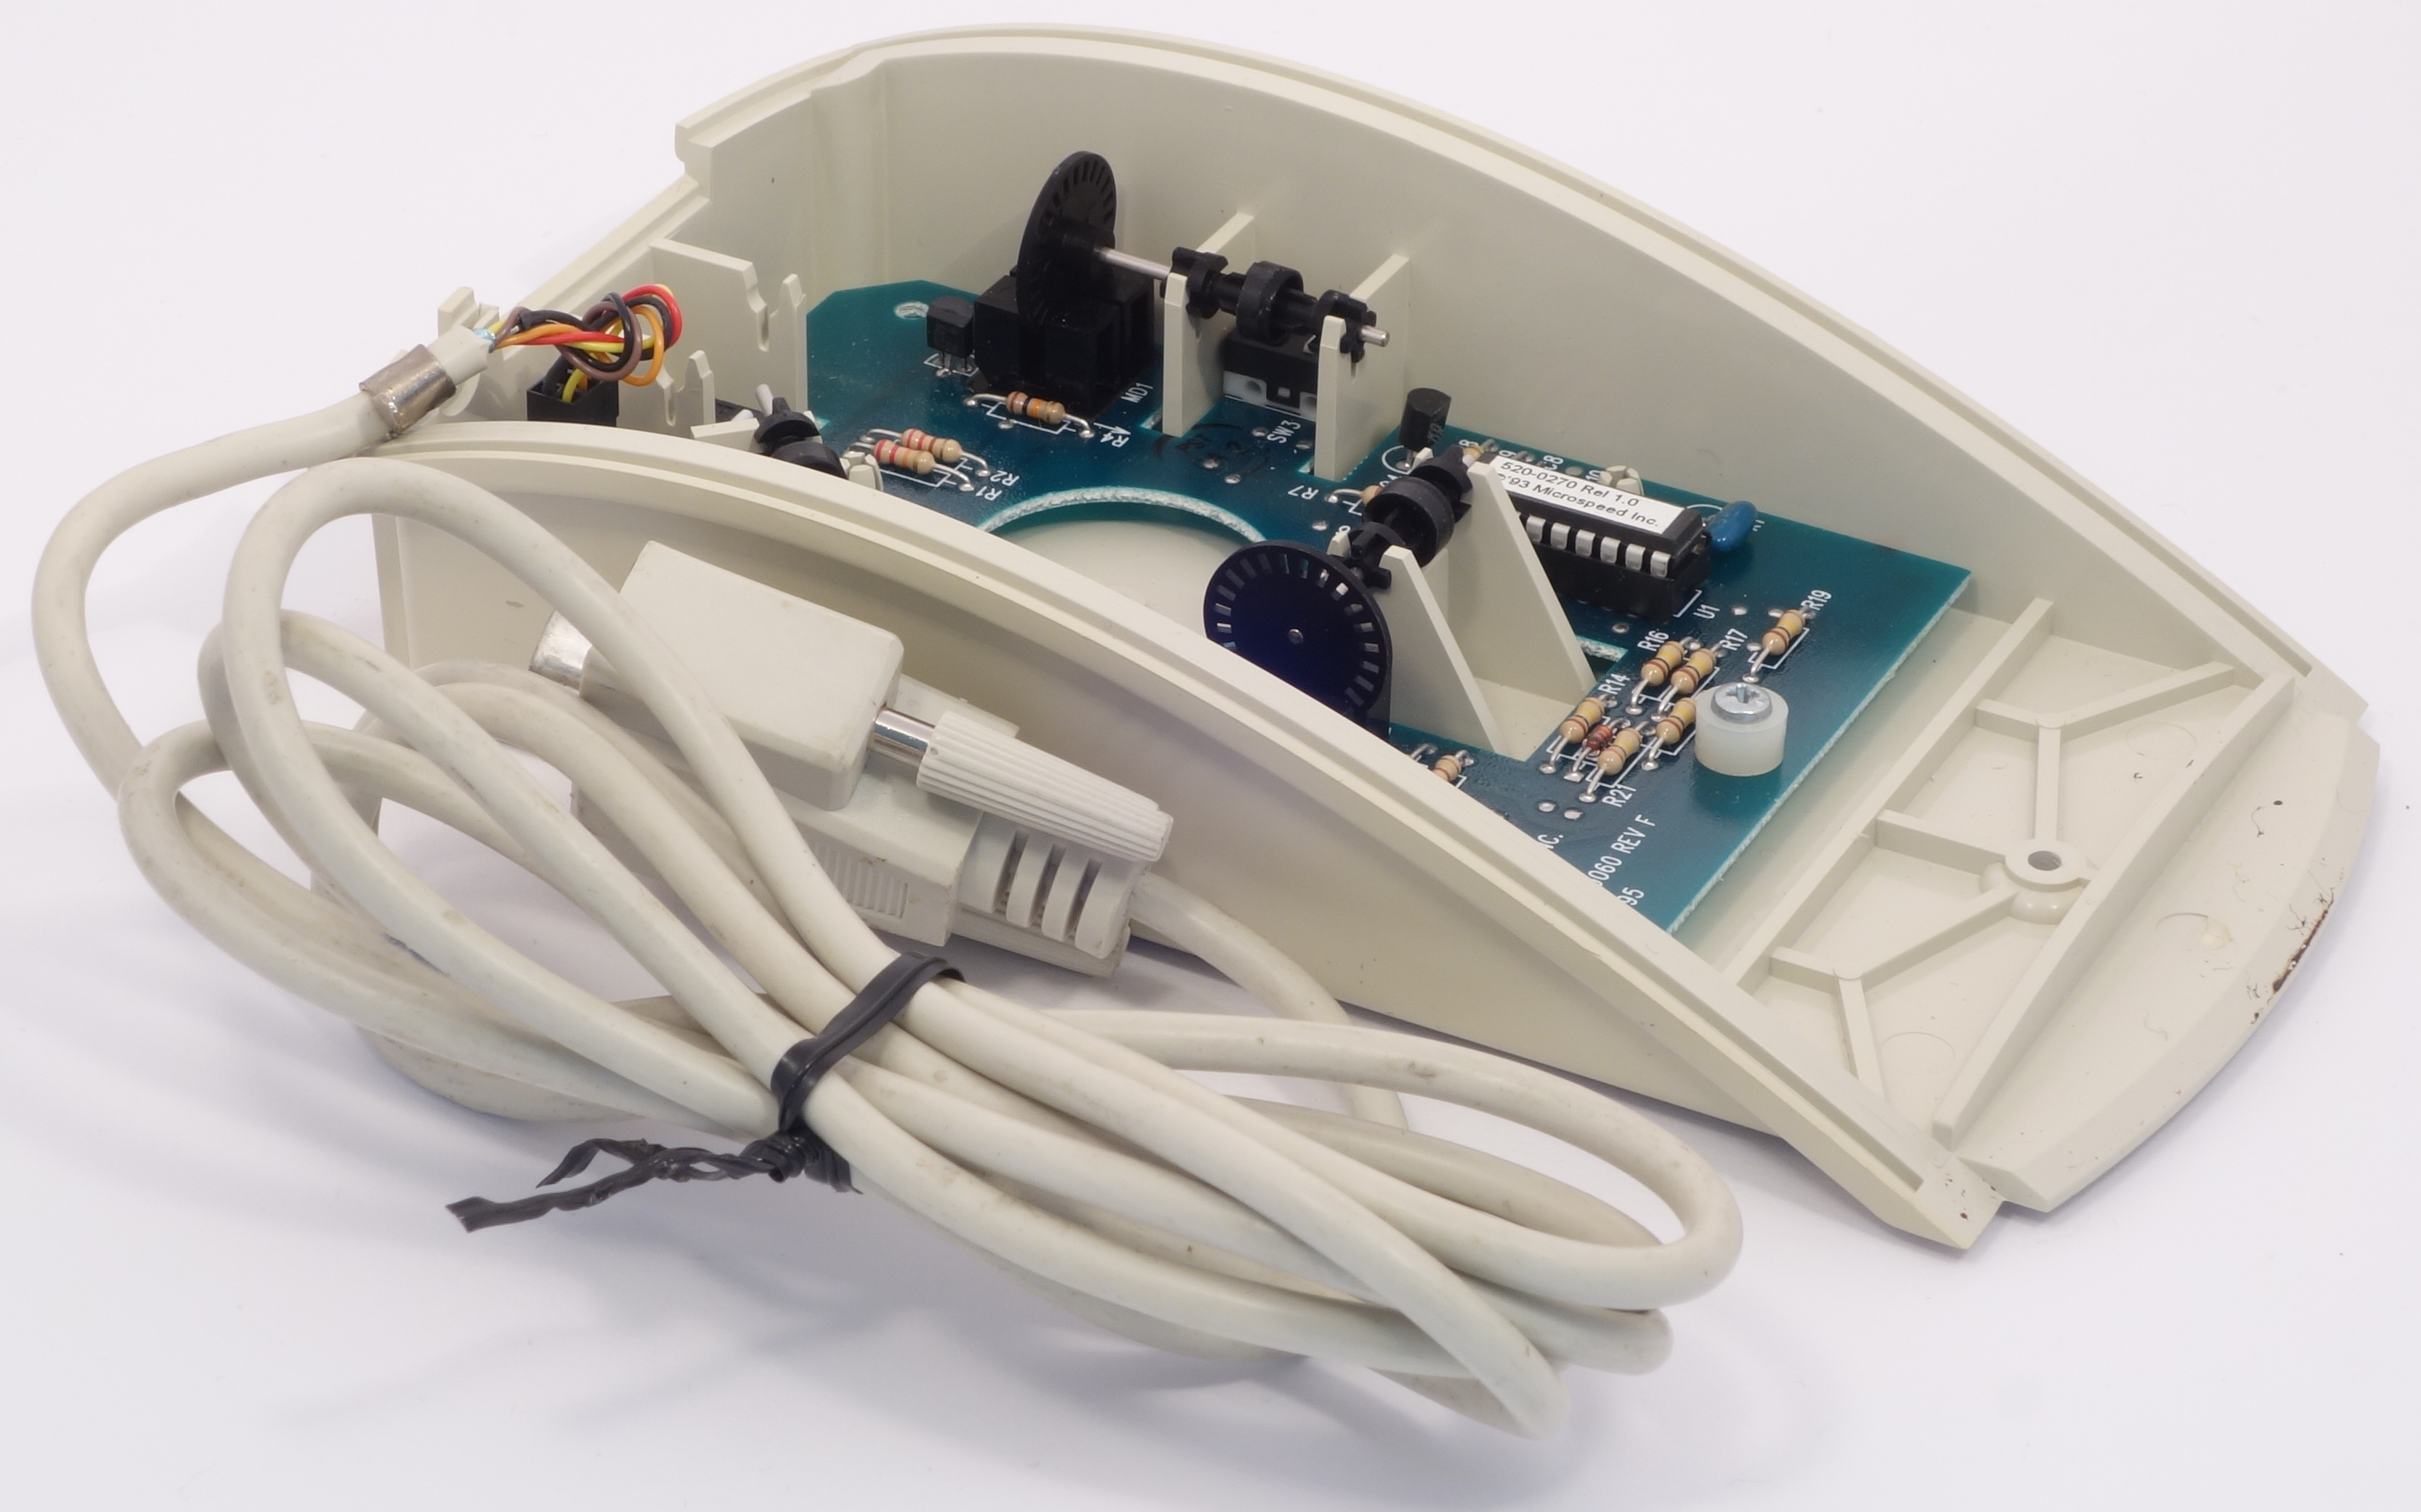
\includegraphics[scale=0.6]{1991_microspeed_pc-track/sony1.jpg}
    \caption{Изображение PC-TRACK в разобранном виде}
    \label{fig:PCTRACKInside}
    \end{figure}

Рисунок \ref{fig:PCTRACKInside} показывает, что трекбол PC-TRACK выполнен по классической оптомеханической схеме. В конструкции роликов MicroSpeed использовала подшипники качения, изготовленные из пластика Delrin. В рекламных материалах отмечалось, что помимо того, что они являются самосмазывающимися, они более устойчивы, чем металлические подшипники, к образованию каверн, загрязнению и повреждениям в результате механических ударов (например, при падении).

\begin{thebibliography}{9}
\bibitem {PC} MiCROSPEED PC-TRACK // Compute! Magazin,  Iss. 132, August 1991. - p. 50.
\end{thebibliography}
\end{document}

\documentclass[11pt, a4paper]{article}
\usepackage{pdfpages}
\usepackage{parallel}
\usepackage[T2A]{fontenc}
\usepackage{ucs}
\usepackage[utf8x]{inputenc}
\usepackage[polish,english,russian]{babel}
\usepackage{hyperref}
\usepackage{rotating}
\usepackage[inner=2cm,top=1.8cm,outer=2cm,bottom=2.3cm,nohead]{geometry}
\usepackage{listings}
\usepackage{graphicx}
\usepackage{wrapfig}
\usepackage{longtable}
\usepackage{indentfirst}
\usepackage{array}
\usepackage{tikzsymbols}
\usepackage{soul}
\usepackage[ruled,vlined]{algorithm2e}
%\counterwithout{figure}{section} 

\usepackage{url}
\makeatletter
\g@addto@macro{\UrlBreaks}{\UrlOrds}
\makeatother

\newcolumntype{P}[1]{>{\raggedright\arraybackslash}p{#1}}
\frenchspacing
\usepackage{fixltx2e} %text sub- and superscripts
\usepackage{icomma} % коскі ў матэматычным рэжыме
\PreloadUnicodePage{4}

\newcommand{\longpage}{\enlargethispage{\baselineskip}}
\newcommand{\shortpage}{\enlargethispage{-\baselineskip}}

\def\switchlang#1{\expandafter\csname switchlang#1\endcsname}
\def\switchlangbe{
\let\saverefname=\refname%
\def\refname{Літаратура}%
\def\figurename{Іл.}%
}
\def\switchlangen{
\let\saverefname=\refname%
\def\refname{References}%
\def\figurename{Fig.}%
}
\def\switchlangru{
\let\saverefname=\refname%
\let\savefigurename=\figurename%
\def\refname{Литература}%
\def\figurename{Рис.}%
}

\hyphenation{admi-ni-stra-tive}
\hyphenation{ex-pe-ri-ence}
\hyphenation{fle-xi-bi-li-ty}
\hyphenation{Py-thon}
\hyphenation{ma-the-ma-ti-cal}
\hyphenation{re-ported}
\hyphenation{imp-le-menta-tions}
\hyphenation{pro-vides}
\hyphenation{en-gi-neering}
\hyphenation{com-pa-ti-bi-li-ty}
\hyphenation{im-pos-sible}
\hyphenation{desk-top}
\hyphenation{elec-tro-nic}
\hyphenation{com-pa-ny}
\hyphenation{de-ve-lop-ment}
\hyphenation{de-ve-loping}
\hyphenation{de-ve-lop}
\hyphenation{da-ta-ba-se}
\hyphenation{plat-forms}
\hyphenation{or-ga-ni-za-tion}
\hyphenation{pro-gramming}
\hyphenation{in-stru-ments}
\hyphenation{Li-nux}
\hyphenation{sour-ce}
\hyphenation{en-vi-ron-ment}
\hyphenation{Te-le-pathy}
\hyphenation{Li-nux-ov-ka}
\hyphenation{Open-BSD}
\hyphenation{Free-BSD}
\hyphenation{men-ti-on-ed}
\hyphenation{app-li-ca-tion}

\def\progref!#1!{\texttt{#1}}
\renewcommand{\arraystretch}{2} %Іначай формулы ў матрыцы зліпаюцца з лініямі
\usepackage{array}

\def\interview #1 (#2), #3, #4, #5\par{

\section[#1, #3, #4]{#1 -- #3, #4}
\def\qname{LVEE}
\def\aname{#1}
\def\q ##1\par{{\noindent \bf \qname: ##1 }\par}
\def\a{{\noindent \bf \aname: } \def\qname{L}\def\aname{#2}}
}

\def\interview* #1 (#2), #3, #4, #5\par{

\section*{#1\\{\small\rm #3, #4. #5}}
\ifx\ParallelWhichBox\undefined%
    \addcontentsline{toc}{section}{#1, #3, #4}%
\else%
\ifnum\ParallelWhichBox=0%
    \addcontentsline{toc}{section}{#1, #3, #4}%
\fi\fi%

\def\qname{LVEE}
\def\aname{#1}
\def\q ##1\par{{\noindent \bf \qname: ##1 }\par}
\def\a{{\noindent \bf \aname: } \def\qname{L}\def\aname{#2}}
}

\newcommand{\interviewfooter}[1]{
\vskip 1em
\noindent \textit{#1}
}


\begin{document}

\title{1992 "--- Трекбол/мышь IBM PS/2 Track Ball}
\date{}
\maketitle
В 1992 году Компания IBM выпустила нестандартный трекбол-перевёртыш, который мог работать в двух режимах: собственно трекбола и обычной мыши (рис. \ref{fig:IBMConvertibleTopAndBottom}). Перевод устройства из одного режима в другой выполняется нажатием на пару пластиковых защёлок, меняющих положение верхней (либо, в зависимости от режима работы, нижней) стенки корпуса, в результате чего шар и расположенные рядом с ним кнопки в большей или в меньшей степени выступают из корпуса.

\begin{figure}[h]
    \centering
    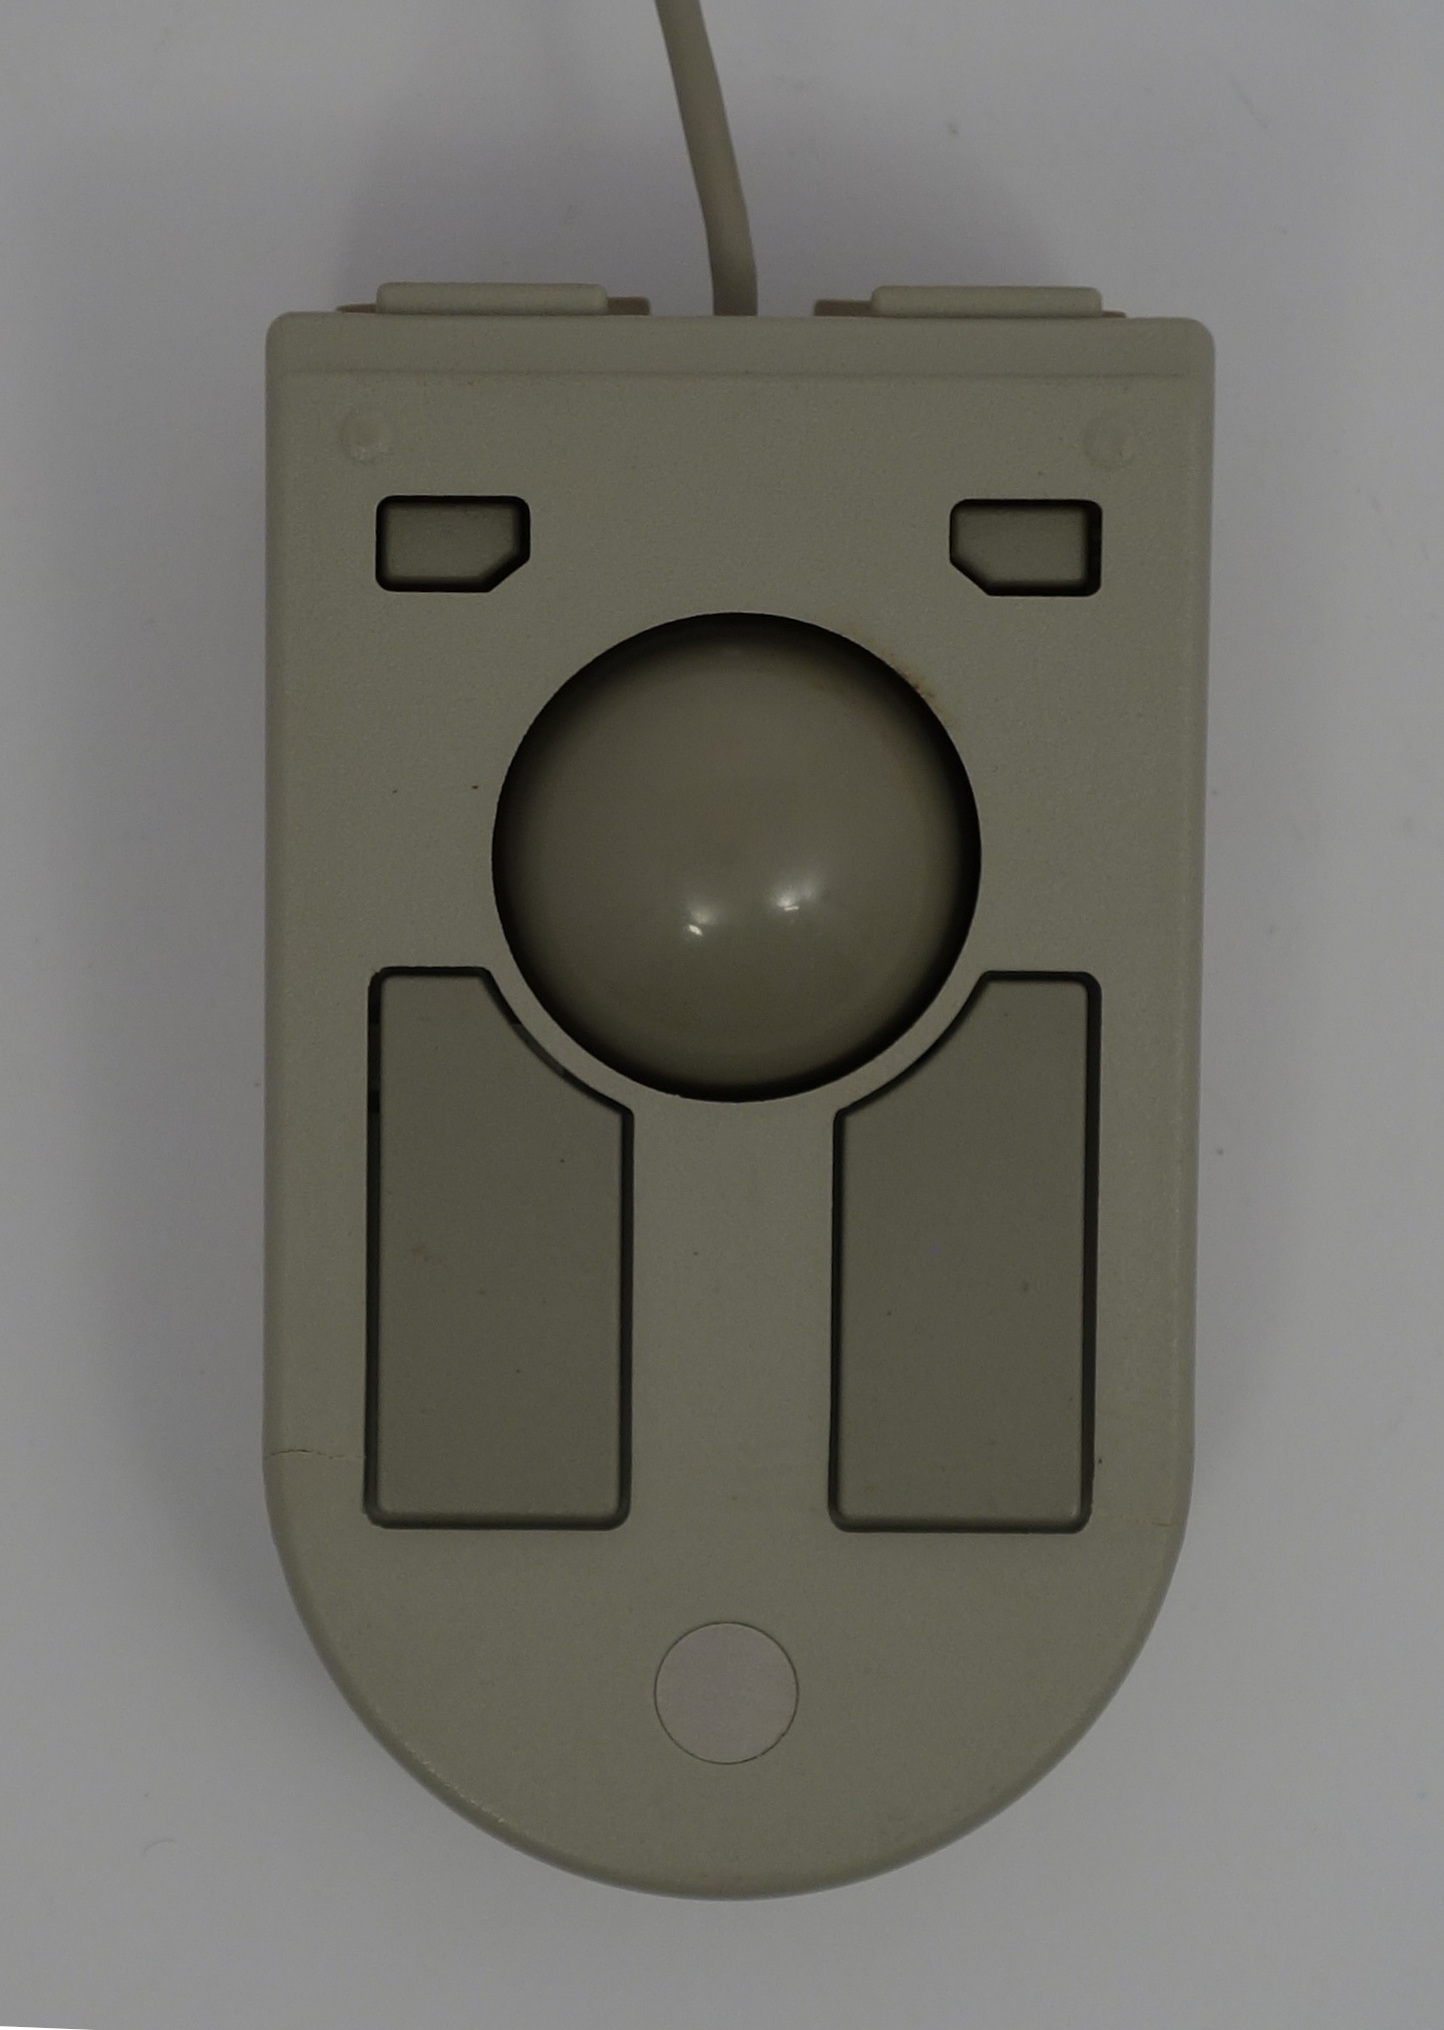
\includegraphics[scale=0.5]{1992_ibm_convertible/2.12.JPG}
    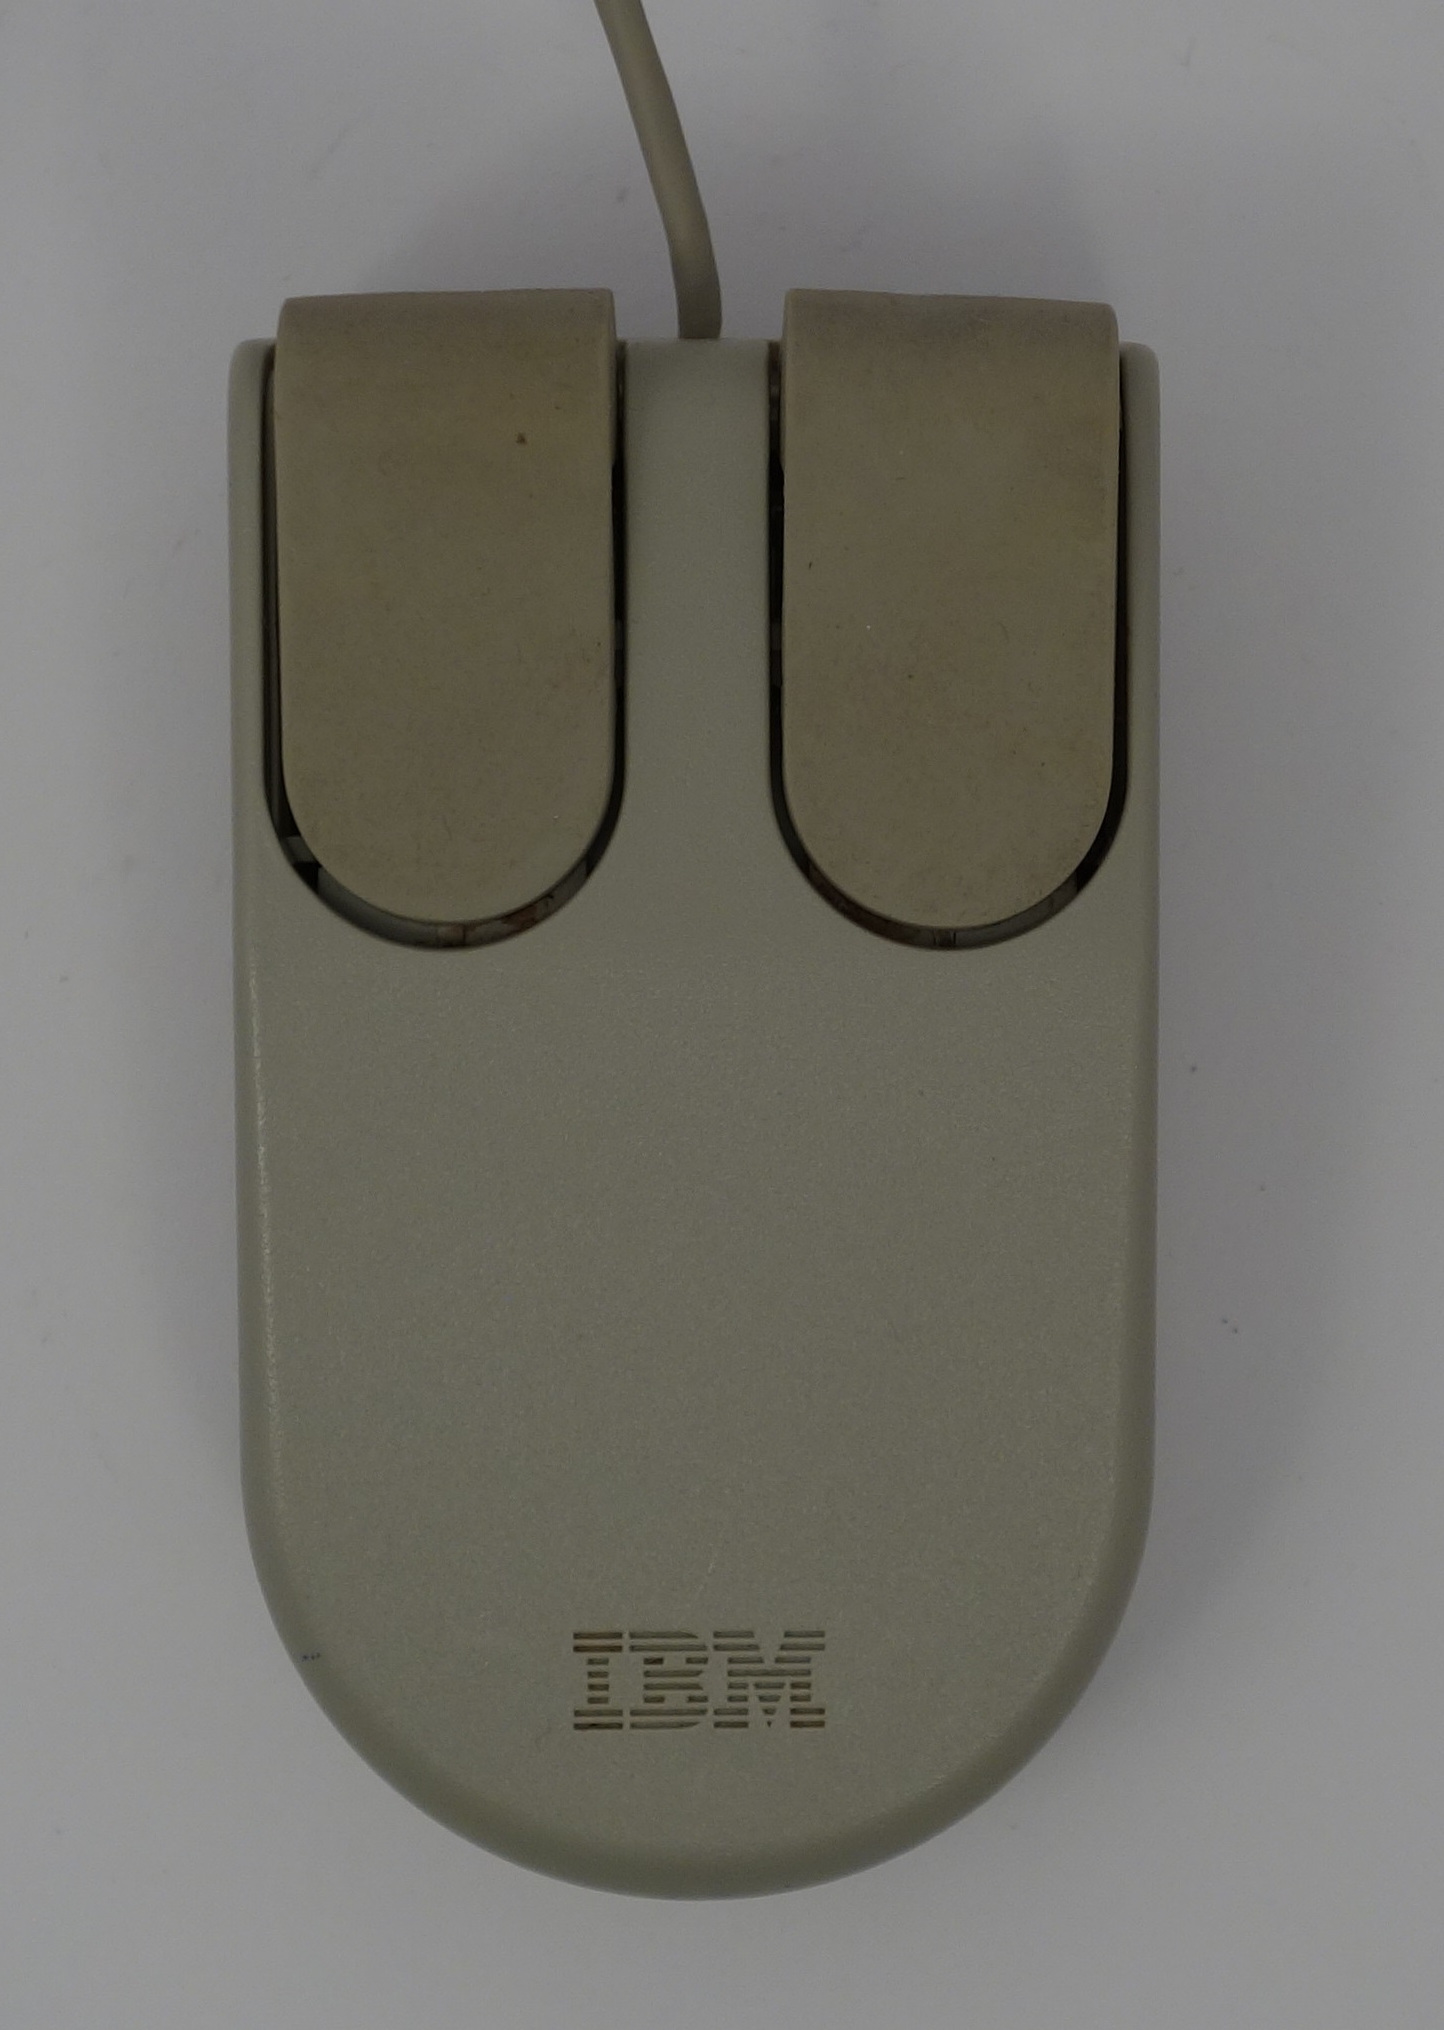
\includegraphics[scale=0.5]{1992_ibm_convertible/2.13.JPG}
    \caption{Изображение IBM PS/2 Track Ball: слева "--- вид трекбола, справа "--- вид мыши}
    \label{fig:IBMConvertibleTopAndBottom}
\end{figure}
    
    Со стороны трекбола на устройстве имеется 4 клавиши: 2 крупные клавиши являются соответственно левой и правой кнопками мыши, 2 маленькие кнопки - это защёлки, нажатие на которые отвечает за блокирование клавиш с противоположной стороны устройства. Со стороны мыши присутствуют логотип IBM и две крупные кнопки.

%\begin{figure}[h]
%    \centering
%    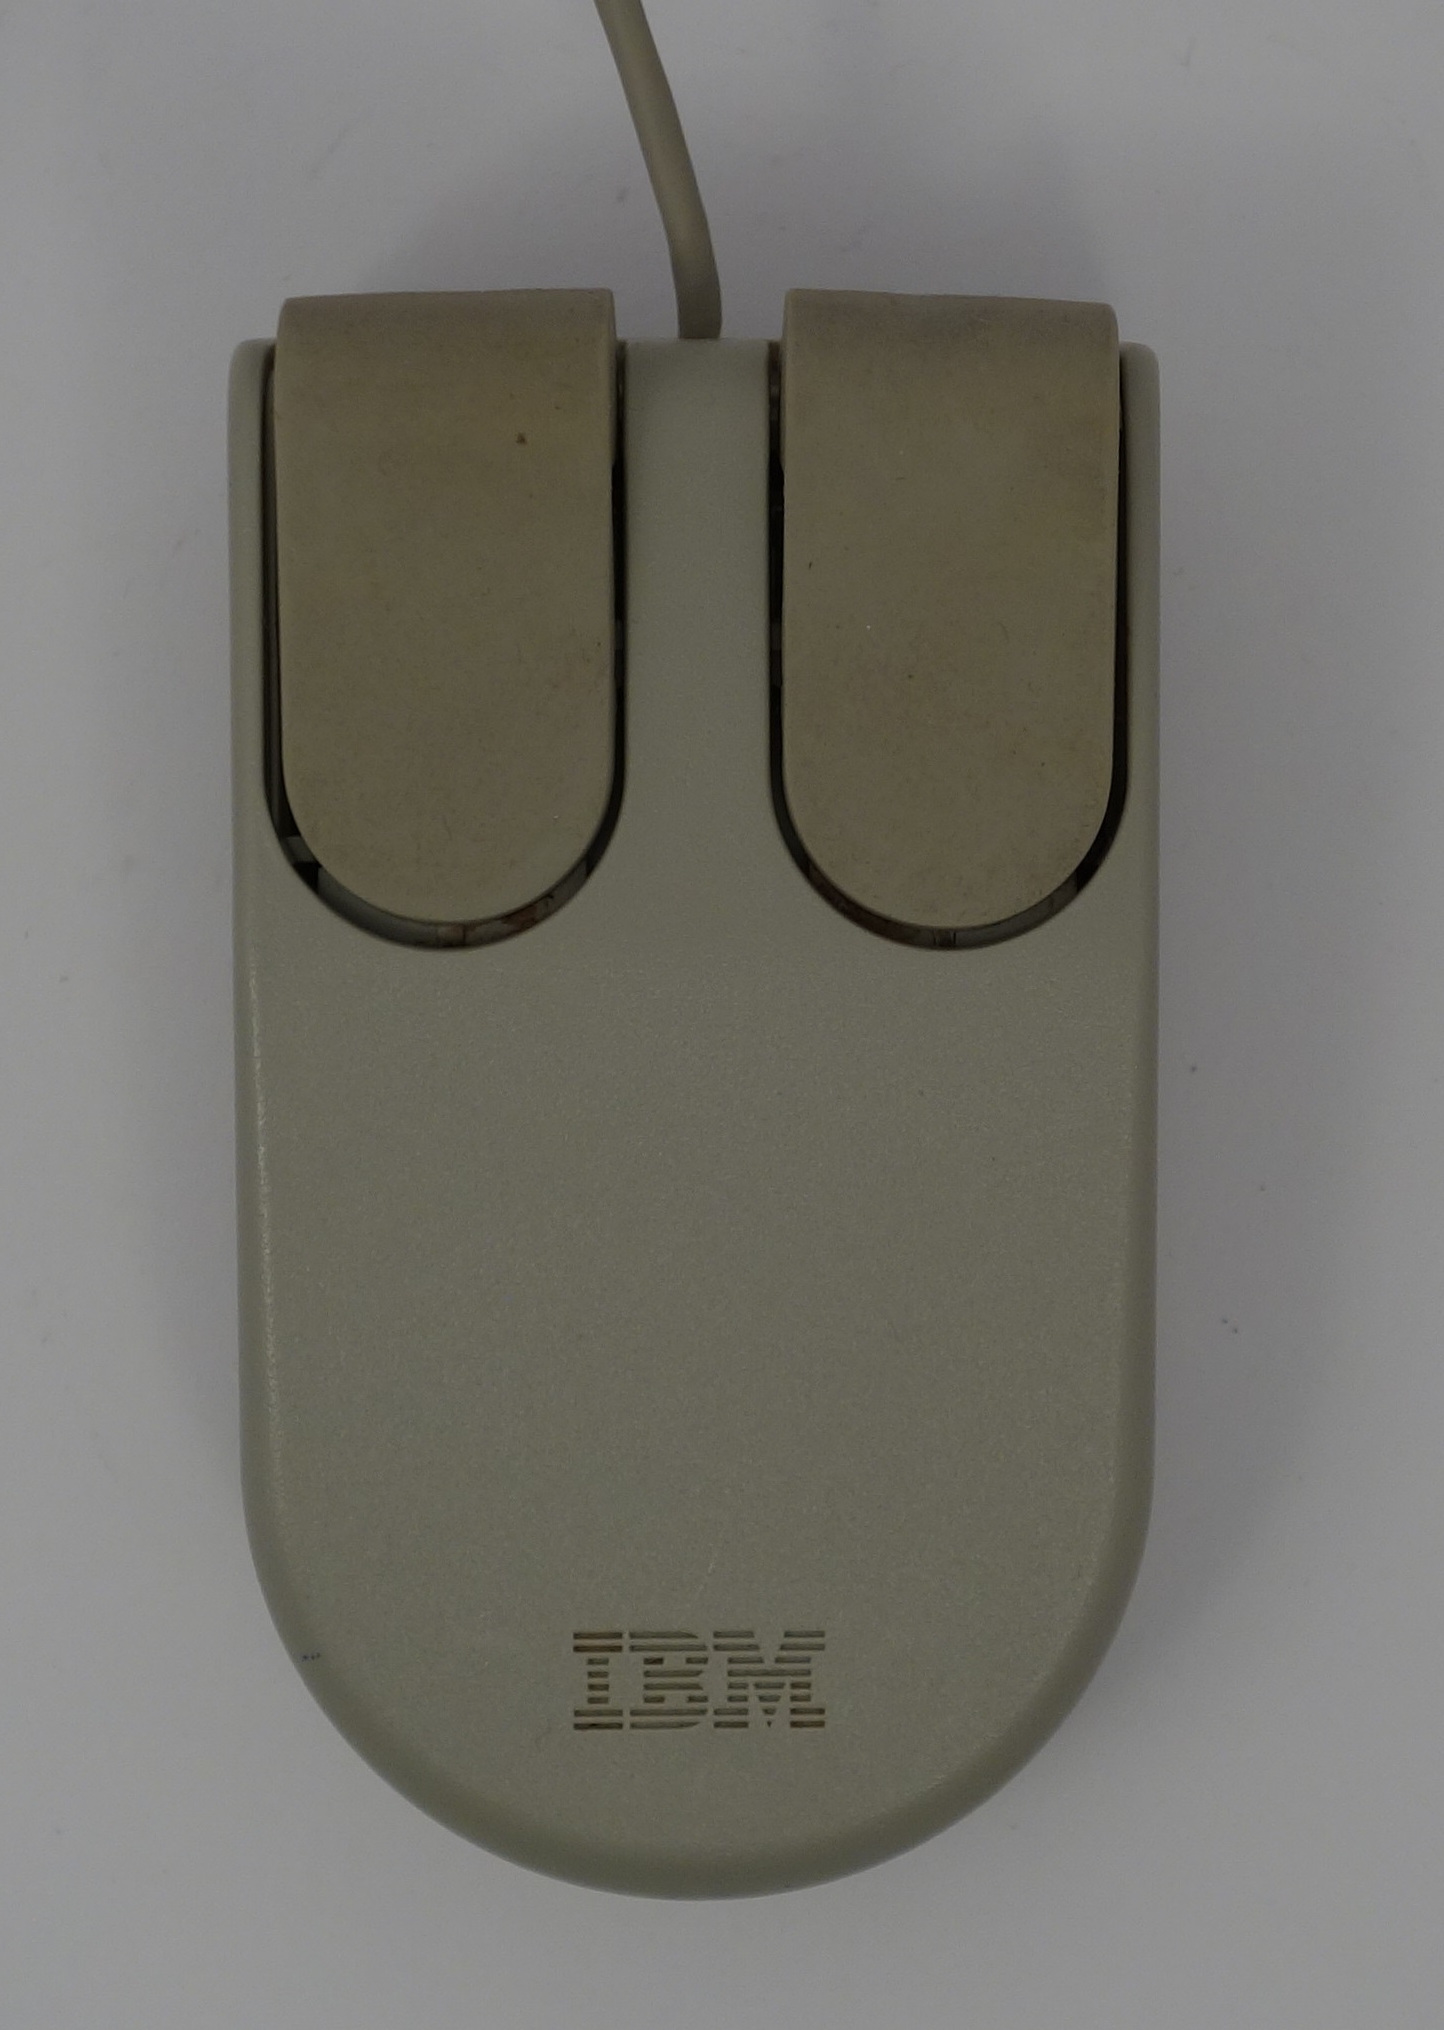
\includegraphics[scale=0.5]{1992_ibm_convertible/2.13.JPG}
%    \caption{Изображение IBM PS/2 Track Ball, вид мыши}
%    \label{fig:IBMConvertibleAsMouse}
%\end{figure}
    
С точки зрения анатомического строения кисти, устройство имеет довольно эргономичную  форму и крупные клавиши, которые удобно нажимать пальцами (рис. \ref{fig:IBMConvertibleHand}). Однако из-за гладкости шара, использование манипулятора в качестве мыши на большинстве поверхностей является  затруднительным. Также оказывается проблемным и его использование в качестве трекбола, поскольку в этом режиме устройство опирается на две выступающие клавиши мыши, что отрицательно сказывается на его устойчивости.

\begin{figure}[h]
    \centering
    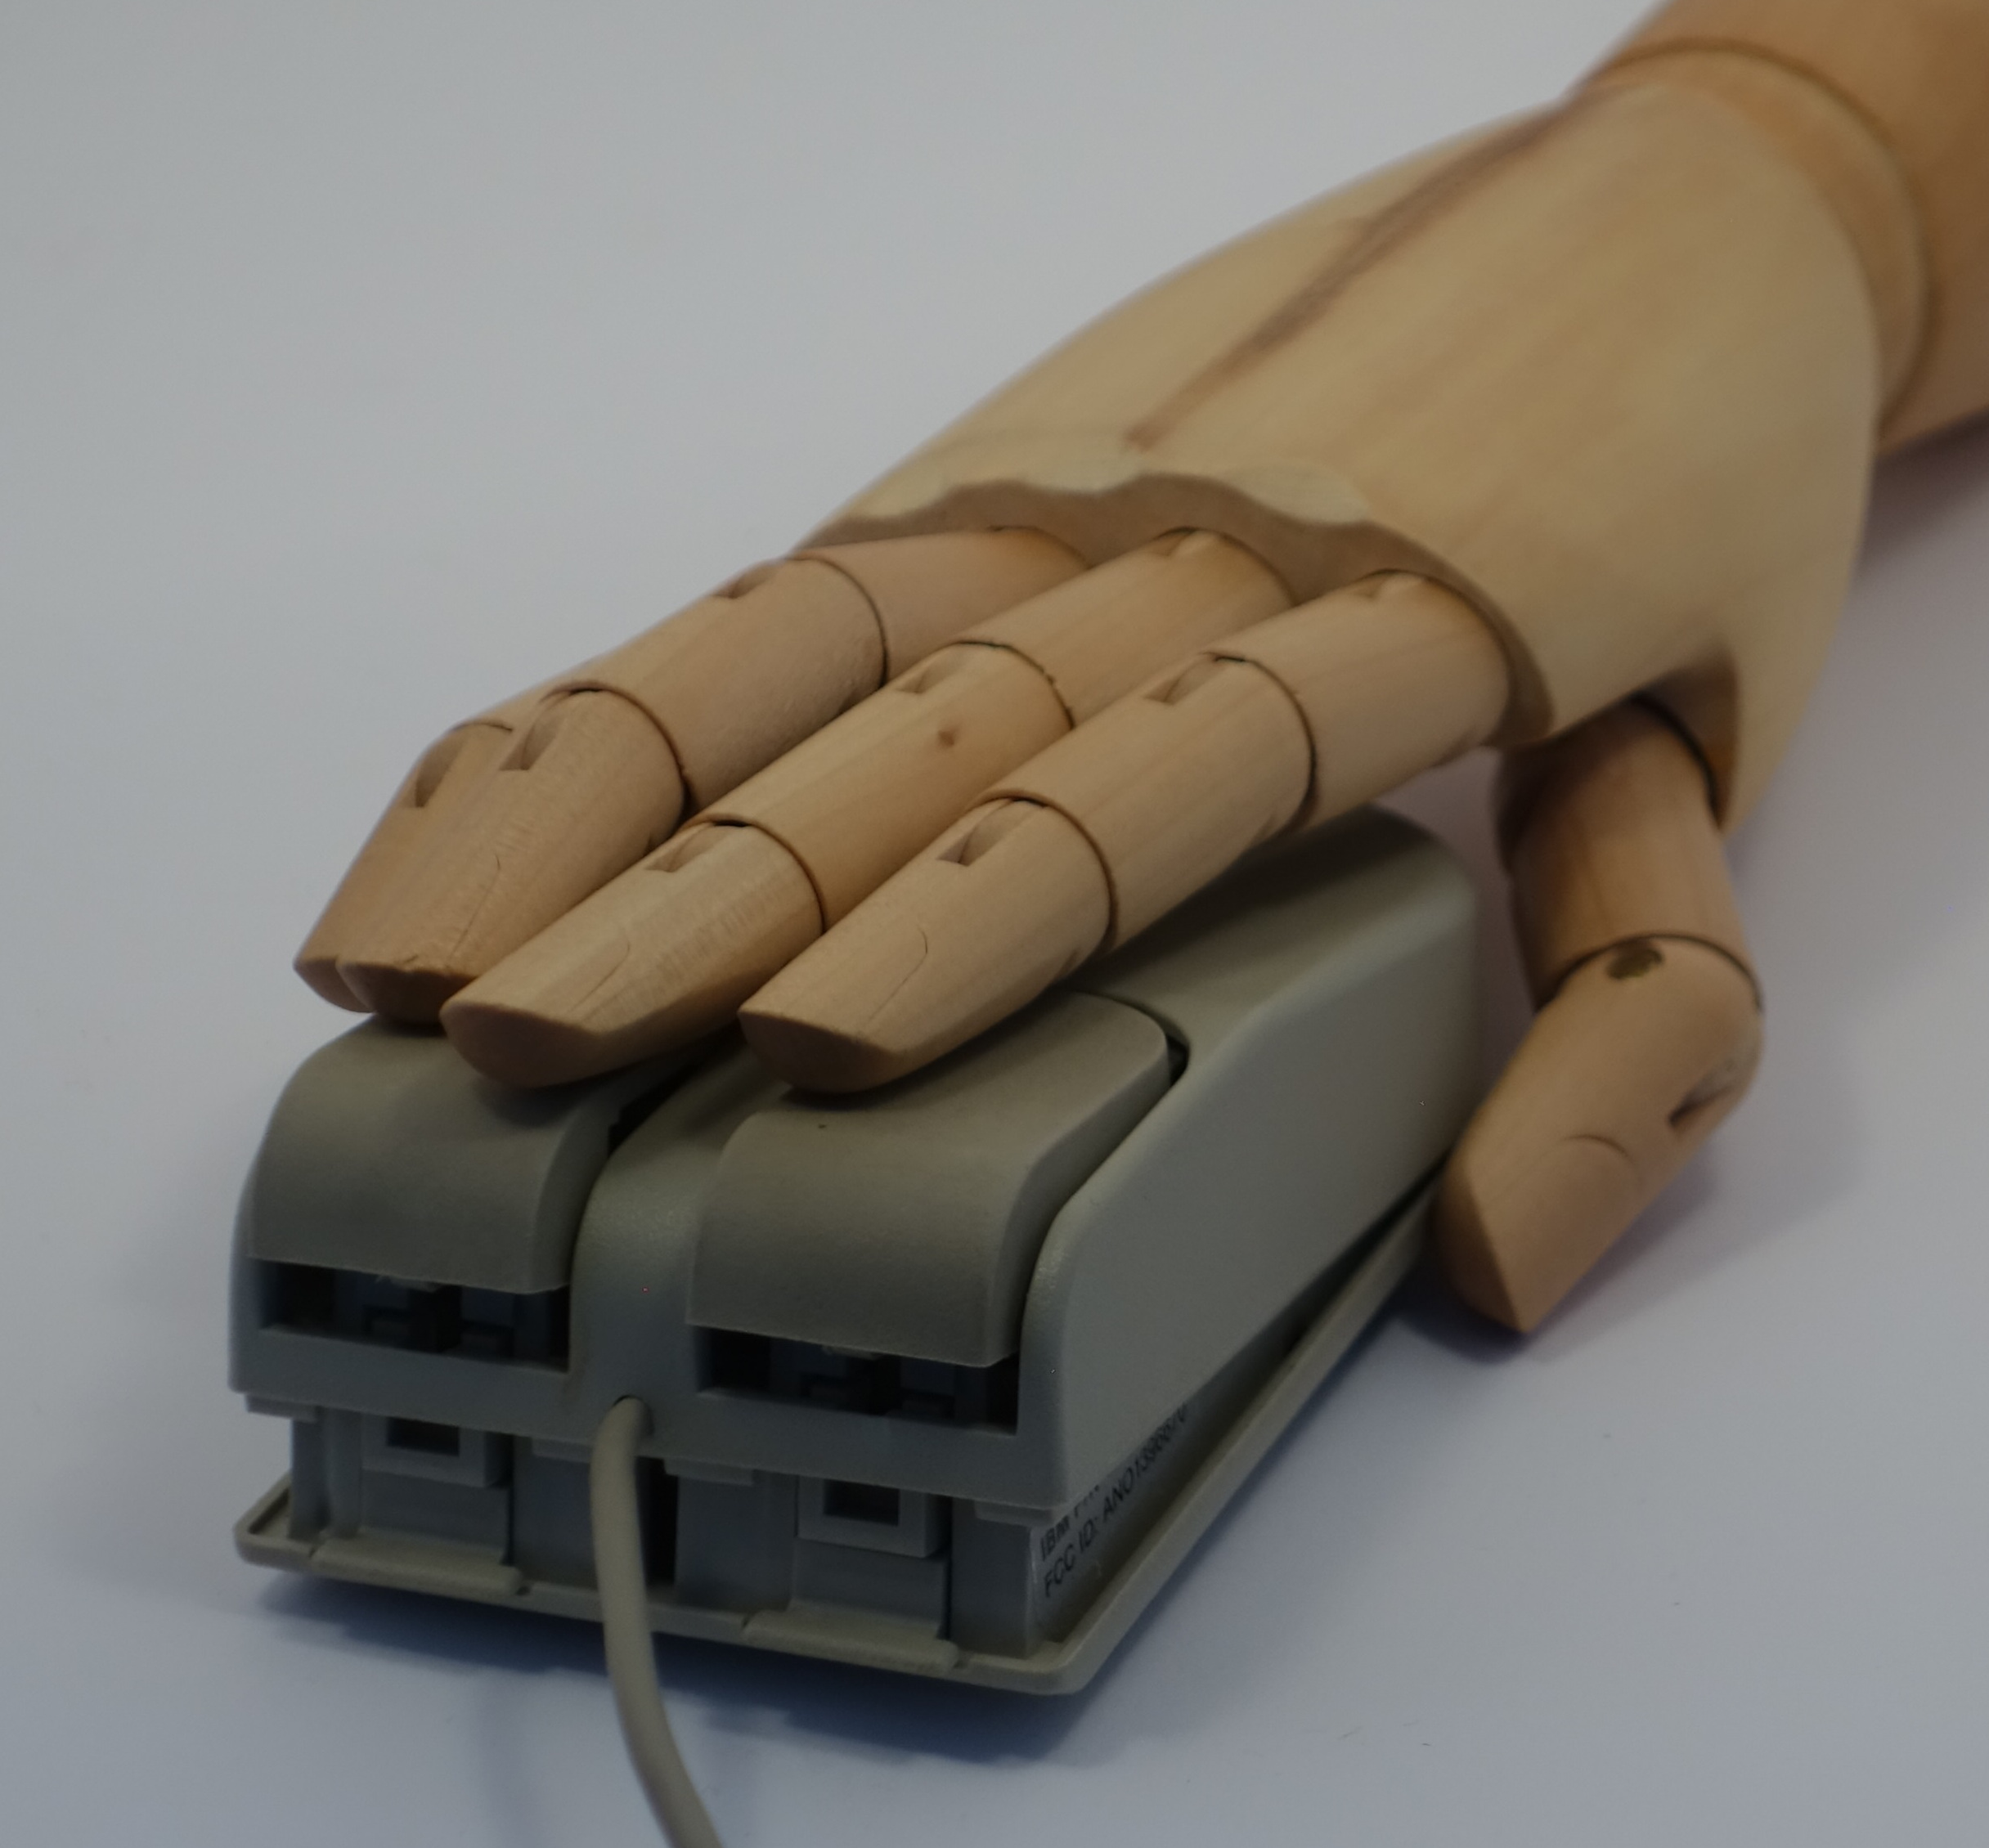
\includegraphics[scale=0.5]{1992_ibm_convertible/2.11.JPG}
    \caption{Изображение BM PS/2 Track Ball с моделью руки человека}
    \label{fig:IBMConvertibleHand}
\end{figure}

Изучение разобранного трекбола показывает, что он также выполнен по стандартной оптомеханической схеме, и имеет надёжные металлические ролики с подшипниками качения (\ref{fig:IBMConvertibleInside}). Для сопряжения данного устройства с компьютером использовался стандартный порт PS/2.

\begin{figure}[h]
    \centering
    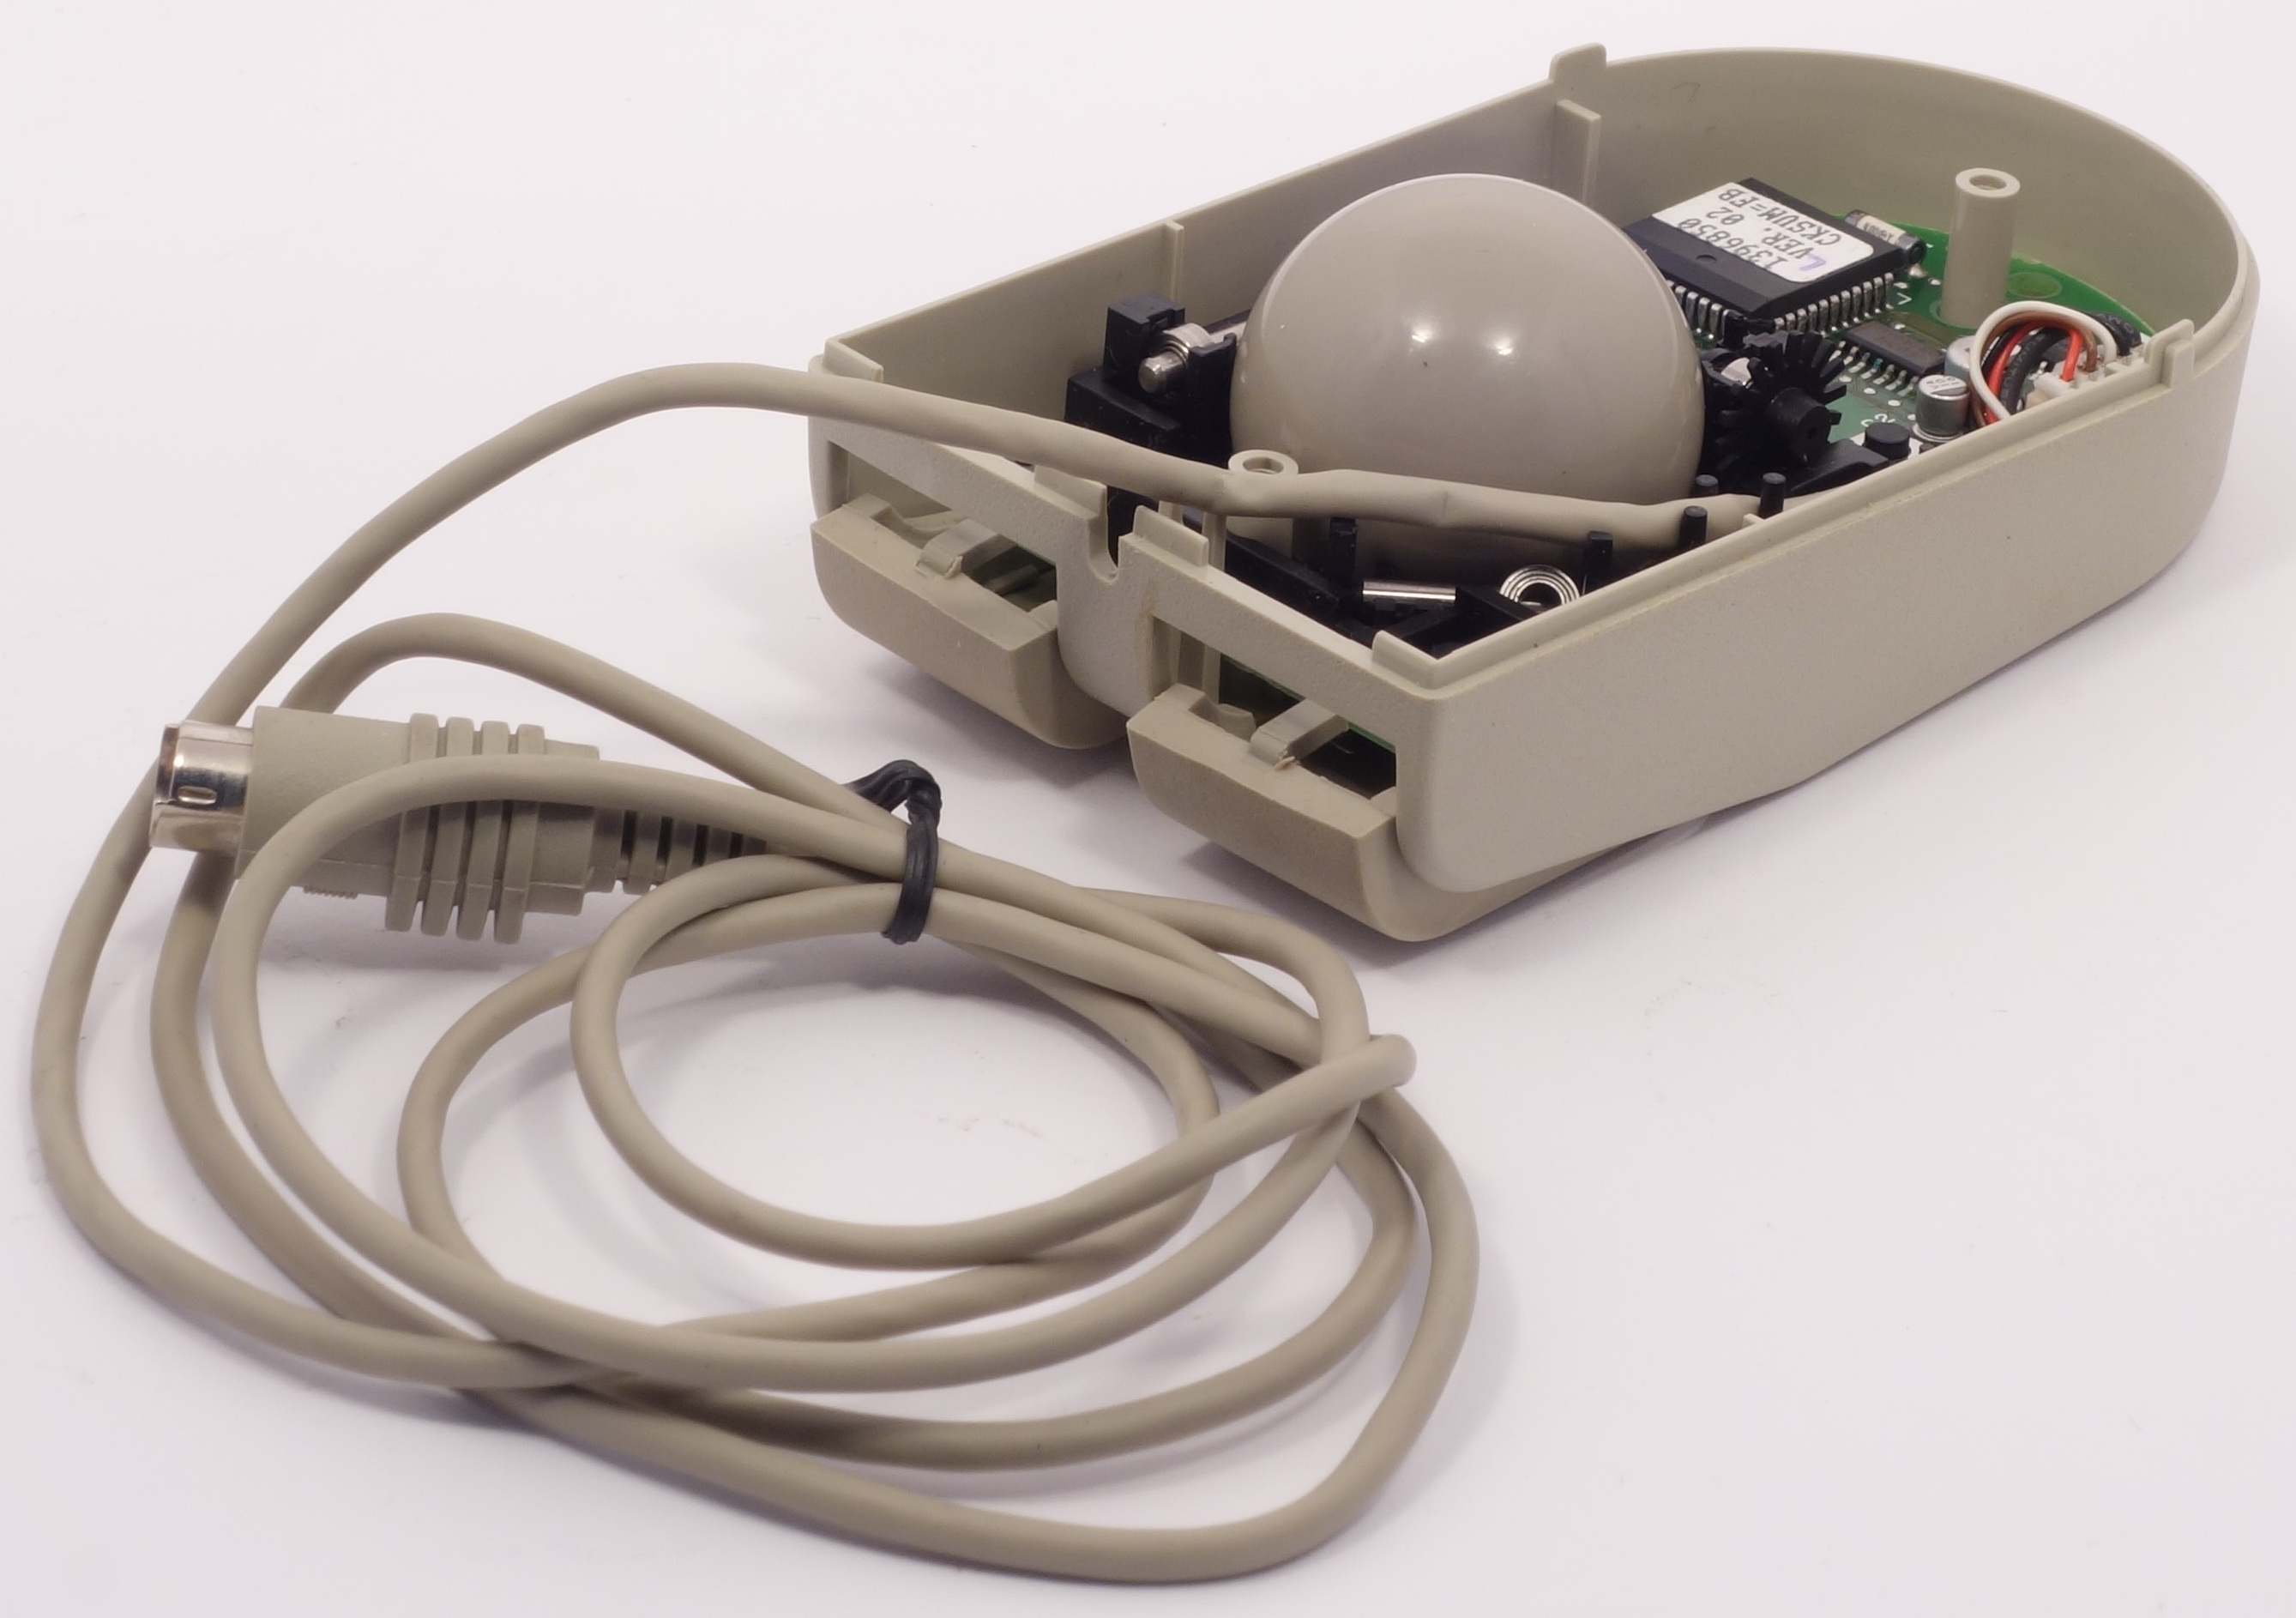
\includegraphics[scale=0.5]{1992_ibm_convertible/202.JPG}
    \caption{Изображение BM PS/2 Track Ball изнутри}
    \label{fig:IBMConvertibleInside}
\end{figure}

Однако в конструкции не предусмотрено способа открыть трекбол для чистки, за исключением отклеивания круглой заглушки, закрывающей доступ к крепежному винту (её можно видеть на рис. \ref{fig:IBMConvertibleTopAndBottom} слева). Учитывая, что попадание мелкого мусора внутрь корпуса механических мышей и трекболов является практически неизбежным, вопрос о длительной эксплуатации данного устройства дополняет его спорные эргономические характеристики.

\begin{thebibliography}{9}
\bibitem {mouses} Quain J.R. IBM PS/2 trackpoint // PC Magazine. October 15, 1991. p. 126
\bibitem {IBM} IBM PS/2 L40SX "Convertible" Pointing Device \url{https://www.youtube.com/watch?v=-OSXeNVM3UI&ab_channel=uxwbill}
\end{thebibliography}
\end{document}

\documentclass[11pt, a4paper]{article}
\usepackage{pdfpages}
\usepackage{parallel}
\usepackage[T2A]{fontenc}
\usepackage{ucs}
\usepackage[utf8x]{inputenc}
\usepackage[polish,english,russian]{babel}
\usepackage{hyperref}
\usepackage{rotating}
\usepackage[inner=2cm,top=1.8cm,outer=2cm,bottom=2.3cm,nohead]{geometry}
\usepackage{listings}
\usepackage{graphicx}
\usepackage{wrapfig}
\usepackage{longtable}
\usepackage{indentfirst}
\usepackage{array}
\usepackage{tikzsymbols}
\usepackage{soul}
\usepackage[ruled,vlined]{algorithm2e}
%\counterwithout{figure}{section} 

\usepackage{url}
\makeatletter
\g@addto@macro{\UrlBreaks}{\UrlOrds}
\makeatother

\newcolumntype{P}[1]{>{\raggedright\arraybackslash}p{#1}}
\frenchspacing
\usepackage{fixltx2e} %text sub- and superscripts
\usepackage{icomma} % коскі ў матэматычным рэжыме
\PreloadUnicodePage{4}

\newcommand{\longpage}{\enlargethispage{\baselineskip}}
\newcommand{\shortpage}{\enlargethispage{-\baselineskip}}

\def\switchlang#1{\expandafter\csname switchlang#1\endcsname}
\def\switchlangbe{
\let\saverefname=\refname%
\def\refname{Літаратура}%
\def\figurename{Іл.}%
}
\def\switchlangen{
\let\saverefname=\refname%
\def\refname{References}%
\def\figurename{Fig.}%
}
\def\switchlangru{
\let\saverefname=\refname%
\let\savefigurename=\figurename%
\def\refname{Литература}%
\def\figurename{Рис.}%
}

\hyphenation{admi-ni-stra-tive}
\hyphenation{ex-pe-ri-ence}
\hyphenation{fle-xi-bi-li-ty}
\hyphenation{Py-thon}
\hyphenation{ma-the-ma-ti-cal}
\hyphenation{re-ported}
\hyphenation{imp-le-menta-tions}
\hyphenation{pro-vides}
\hyphenation{en-gi-neering}
\hyphenation{com-pa-ti-bi-li-ty}
\hyphenation{im-pos-sible}
\hyphenation{desk-top}
\hyphenation{elec-tro-nic}
\hyphenation{com-pa-ny}
\hyphenation{de-ve-lop-ment}
\hyphenation{de-ve-loping}
\hyphenation{de-ve-lop}
\hyphenation{da-ta-ba-se}
\hyphenation{plat-forms}
\hyphenation{or-ga-ni-za-tion}
\hyphenation{pro-gramming}
\hyphenation{in-stru-ments}
\hyphenation{Li-nux}
\hyphenation{sour-ce}
\hyphenation{en-vi-ron-ment}
\hyphenation{Te-le-pathy}
\hyphenation{Li-nux-ov-ka}
\hyphenation{Open-BSD}
\hyphenation{Free-BSD}
\hyphenation{men-ti-on-ed}
\hyphenation{app-li-ca-tion}

\def\progref!#1!{\texttt{#1}}
\renewcommand{\arraystretch}{2} %Іначай формулы ў матрыцы зліпаюцца з лініямі
\usepackage{array}

\def\interview #1 (#2), #3, #4, #5\par{

\section[#1, #3, #4]{#1 -- #3, #4}
\def\qname{LVEE}
\def\aname{#1}
\def\q ##1\par{{\noindent \bf \qname: ##1 }\par}
\def\a{{\noindent \bf \aname: } \def\qname{L}\def\aname{#2}}
}

\def\interview* #1 (#2), #3, #4, #5\par{

\section*{#1\\{\small\rm #3, #4. #5}}
\ifx\ParallelWhichBox\undefined%
    \addcontentsline{toc}{section}{#1, #3, #4}%
\else%
\ifnum\ParallelWhichBox=0%
    \addcontentsline{toc}{section}{#1, #3, #4}%
\fi\fi%

\def\qname{LVEE}
\def\aname{#1}
\def\q ##1\par{{\noindent \bf \qname: ##1 }\par}
\def\a{{\noindent \bf \aname: } \def\qname{L}\def\aname{#2}}
}

\newcommand{\interviewfooter}[1]{
\vskip 1em
\noindent \textit{#1}
}


\begin{document}

\title{1993 "--- Easy Options trackball}
\date{}
\maketitle

Наиболее заметной визуальной особенностью трекбола Easy Options является дизайн в стиле бытовых приборов 60-х годов (рис. \ref{fig:EasyOptionsPic}).

\begin{figure}[h]
    \centering
    \includegraphics[scale=0.7]{1993_easy_options_trackball/pic_60.jpg}
    \caption{Трекбол Easy Options}
    \label{fig:EasyOptionsPic}
\end{figure}

Перевернув устройство, можно увидеть код FCC ID (рис. \ref{fig:EasyOptionsTopBottom}), исследование которого показывает, что трекбол производился тайваньской компанией начиная с 1993 года.

\begin{figure}[h]
    \centering
    \includegraphics[scale=0.6]{1993_easy_options_trackball/top_60.jpg}
    \includegraphics[scale=0.6]{1993_easy_options_trackball/bottom_60.jpg}
    \caption{Easy Options, вид сверху и снизу}
    \label{fig:EasyOptionsTopBottom}
\end{figure}

Как можно видеть на рис. \ref{fig:EasyOptionsSize}, этот манипулятор имеет сравнительно небольшие размеры.

\begin{figure}[h]
    \centering
    \includegraphics[scale=0.35]{1993_easy_options_trackball/size_30.jpg}
    \caption{Easy Options на размерном коврике с шагом сетки 1 см}
    \label{fig:EasyOptionsSize}
\end{figure}

В плане эргономики можно отметить закруглённые формы корпуса, практически не имеющего острых углов, а также левую и правую кнопки, занимающие всю его длину, что достаточно хорошо согласуется с анатомическим строением кисти (рис. \ref{fig:EasyOptionsHand}).

\begin{figure}[h]
    \centering
    \includegraphics[scale=0.35]{1993_easy_options_trackball/hand_30.jpg}
    \caption{Easy Options в комплекте с моделью руки человека}
    \label{fig:EasyOptionsHand}
\end{figure}

В Easy Options также используется специальная кнопка, которая позволяет включить либо отключить все остальные кнопки во избежание случайного нажатия и для удобного перемещения курсора мыши соответственно. Еще одной отличительной особенностью манипулятора является двусторонний разъём, позволяющий подключаться к последовательному порту, оснащенному гнездом как с 9, так и с 25 контактами.

\begin{figure}[h]
    \centering
    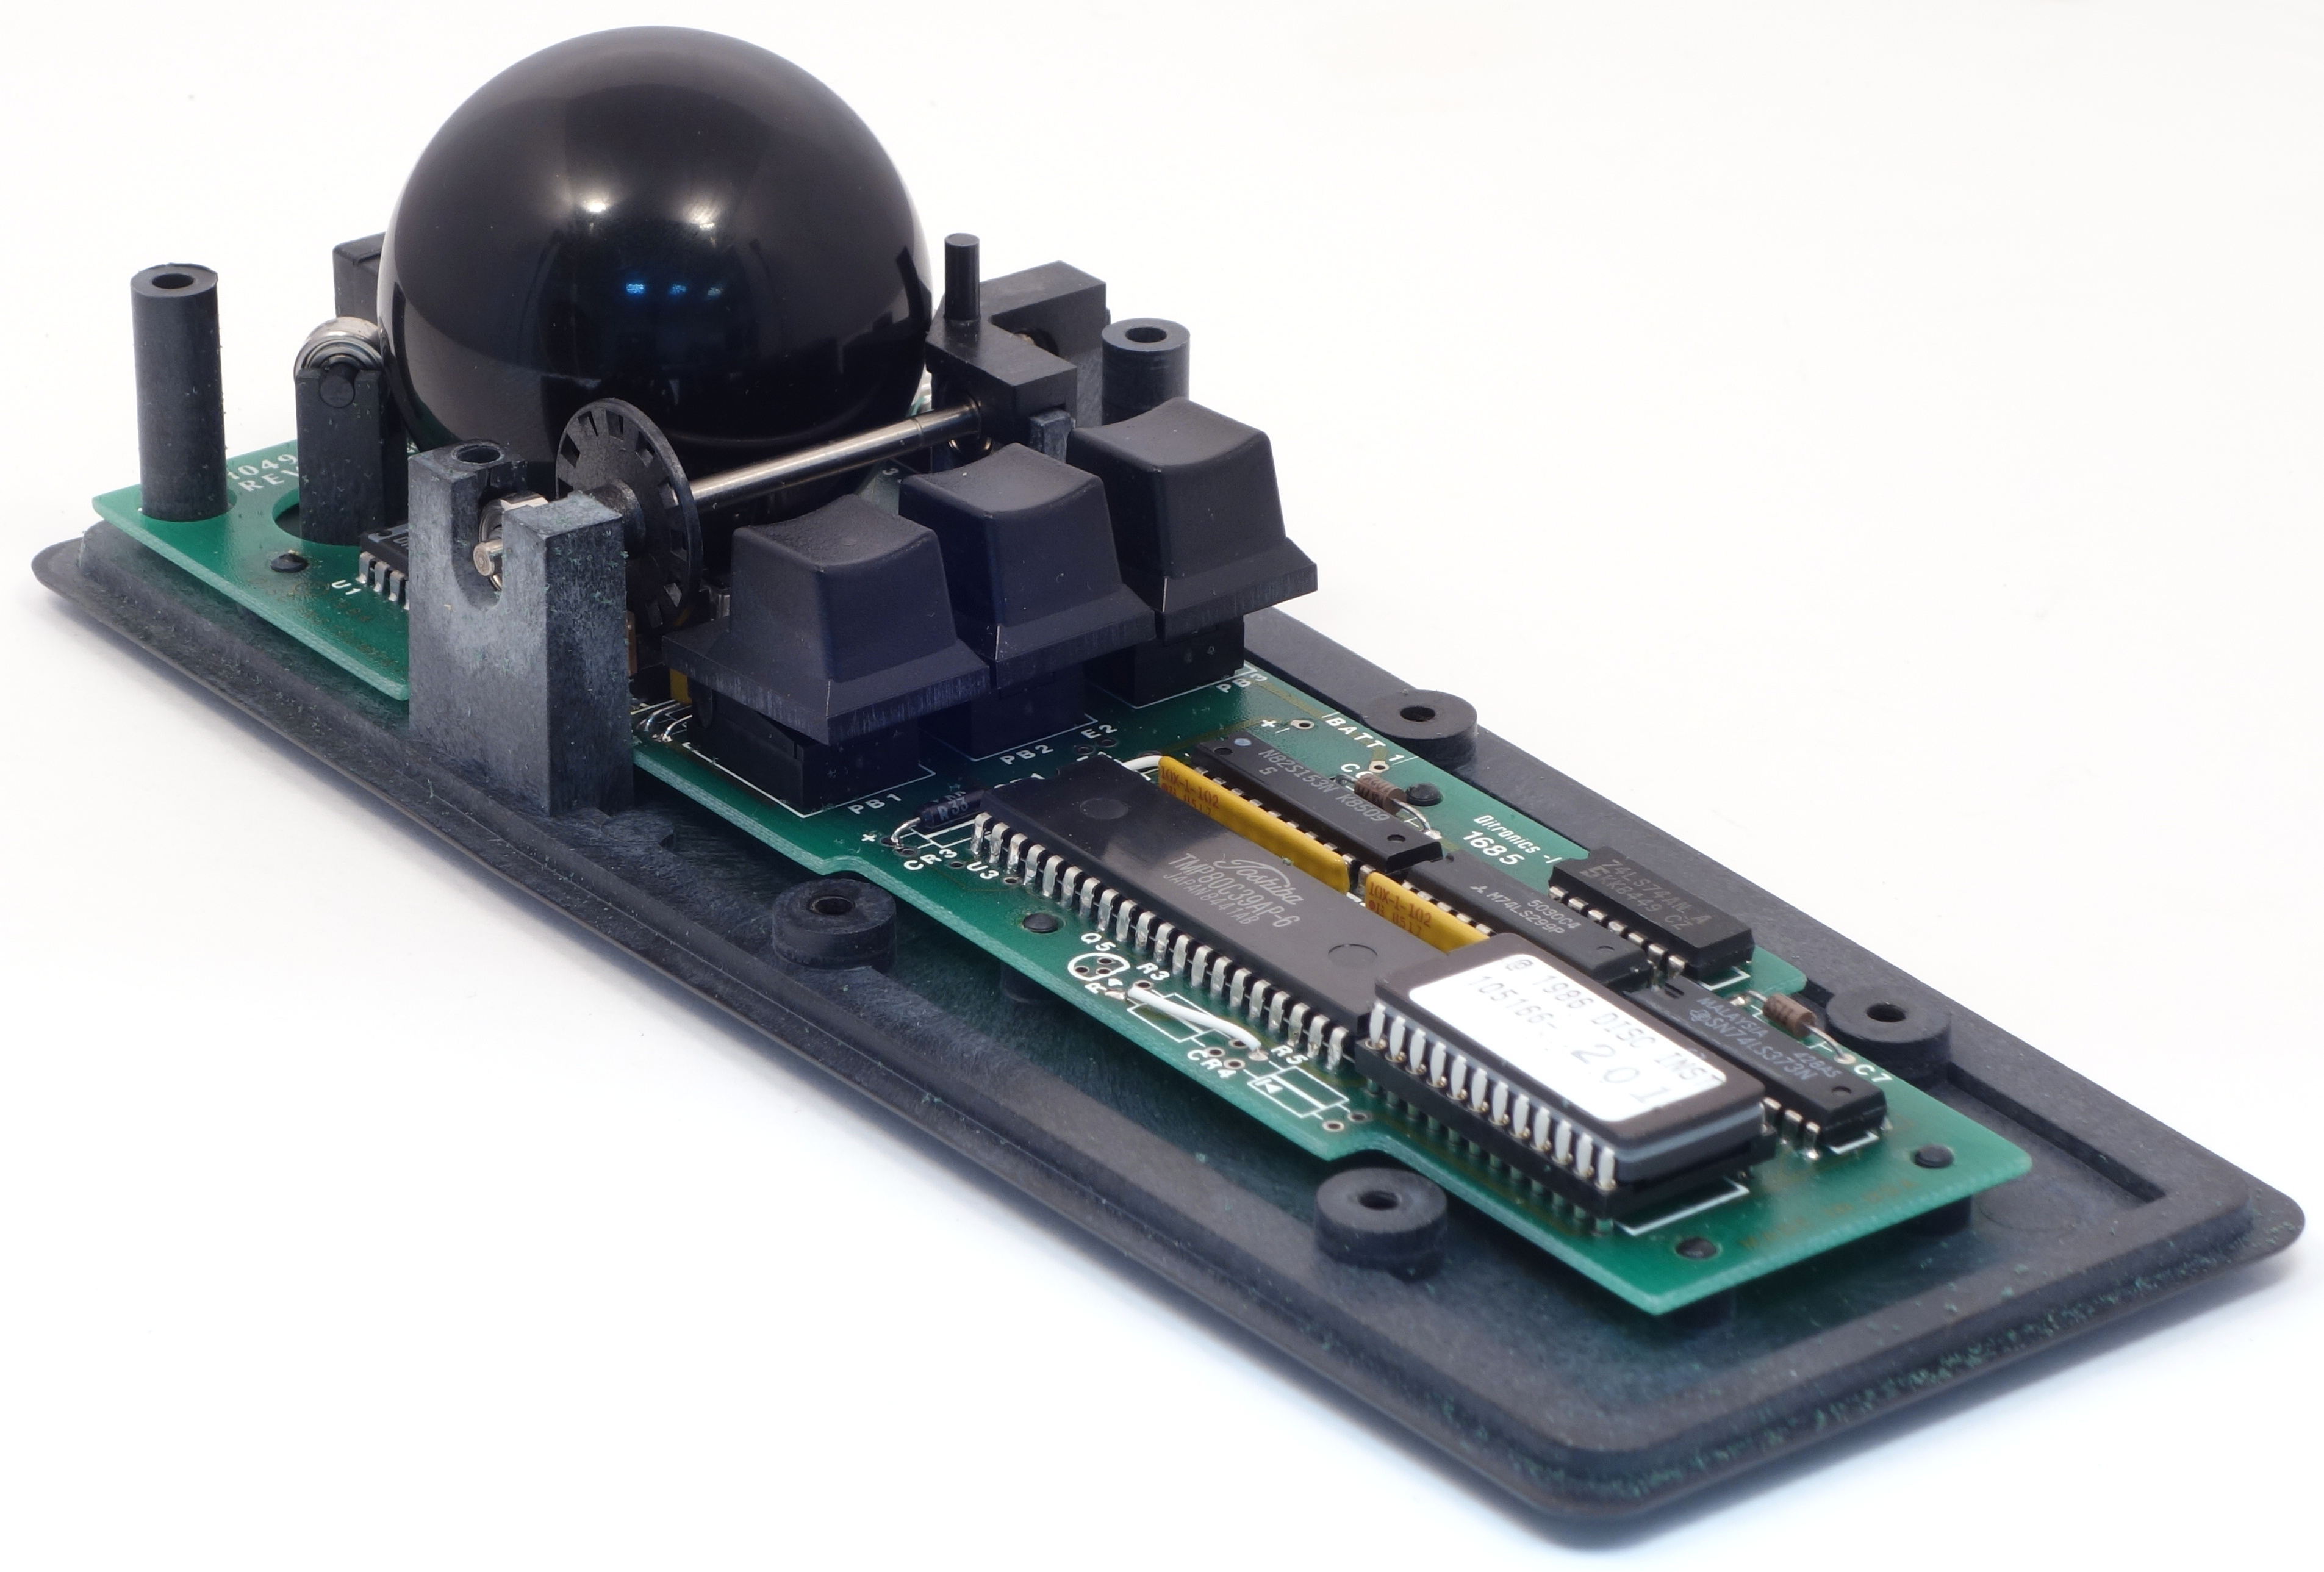
\includegraphics[scale=0.6]{1993_easy_options_trackball/inside_60.jpg}
    \caption{Easy Options в разобранном виде}
    \label{fig:EasyOptionsInside}
\end{figure}

Рисунок \ref{fig:EasyOptionsInside} показывает, что манипулятор выполнен по классической оптомеханической схеме. Из особенностей конструкции можно отметить четыре пружины, обеспечивающие равномерный ход вытянутым в длину левой и правой клавишам, а также подпружиненную центральную клавишу.

\end{document}

\documentclass[11pt, a4paper]{article}
\usepackage{pdfpages}
\usepackage{parallel}
\usepackage[T2A]{fontenc}
\usepackage{ucs}
\usepackage[utf8x]{inputenc}
\usepackage[polish,english,russian]{babel}
\usepackage{hyperref}
\usepackage{rotating}
\usepackage[inner=2cm,top=1.8cm,outer=2cm,bottom=2.3cm,nohead]{geometry}
\usepackage{listings}
\usepackage{graphicx}
\usepackage{wrapfig}
\usepackage{longtable}
\usepackage{indentfirst}
\usepackage{array}
\usepackage{tikzsymbols}
\usepackage{soul}
\usepackage[ruled,vlined]{algorithm2e}
%\counterwithout{figure}{section} 

\usepackage{url}
\makeatletter
\g@addto@macro{\UrlBreaks}{\UrlOrds}
\makeatother

\newcolumntype{P}[1]{>{\raggedright\arraybackslash}p{#1}}
\frenchspacing
\usepackage{fixltx2e} %text sub- and superscripts
\usepackage{icomma} % коскі ў матэматычным рэжыме
\PreloadUnicodePage{4}

\newcommand{\longpage}{\enlargethispage{\baselineskip}}
\newcommand{\shortpage}{\enlargethispage{-\baselineskip}}

\def\switchlang#1{\expandafter\csname switchlang#1\endcsname}
\def\switchlangbe{
\let\saverefname=\refname%
\def\refname{Літаратура}%
\def\figurename{Іл.}%
}
\def\switchlangen{
\let\saverefname=\refname%
\def\refname{References}%
\def\figurename{Fig.}%
}
\def\switchlangru{
\let\saverefname=\refname%
\let\savefigurename=\figurename%
\def\refname{Литература}%
\def\figurename{Рис.}%
}

\hyphenation{admi-ni-stra-tive}
\hyphenation{ex-pe-ri-ence}
\hyphenation{fle-xi-bi-li-ty}
\hyphenation{Py-thon}
\hyphenation{ma-the-ma-ti-cal}
\hyphenation{re-ported}
\hyphenation{imp-le-menta-tions}
\hyphenation{pro-vides}
\hyphenation{en-gi-neering}
\hyphenation{com-pa-ti-bi-li-ty}
\hyphenation{im-pos-sible}
\hyphenation{desk-top}
\hyphenation{elec-tro-nic}
\hyphenation{com-pa-ny}
\hyphenation{de-ve-lop-ment}
\hyphenation{de-ve-loping}
\hyphenation{de-ve-lop}
\hyphenation{da-ta-ba-se}
\hyphenation{plat-forms}
\hyphenation{or-ga-ni-za-tion}
\hyphenation{pro-gramming}
\hyphenation{in-stru-ments}
\hyphenation{Li-nux}
\hyphenation{sour-ce}
\hyphenation{en-vi-ron-ment}
\hyphenation{Te-le-pathy}
\hyphenation{Li-nux-ov-ka}
\hyphenation{Open-BSD}
\hyphenation{Free-BSD}
\hyphenation{men-ti-on-ed}
\hyphenation{app-li-ca-tion}

\def\progref!#1!{\texttt{#1}}
\renewcommand{\arraystretch}{2} %Іначай формулы ў матрыцы зліпаюцца з лініямі
\usepackage{array}

\def\interview #1 (#2), #3, #4, #5\par{

\section[#1, #3, #4]{#1 -- #3, #4}
\def\qname{LVEE}
\def\aname{#1}
\def\q ##1\par{{\noindent \bf \qname: ##1 }\par}
\def\a{{\noindent \bf \aname: } \def\qname{L}\def\aname{#2}}
}

\def\interview* #1 (#2), #3, #4, #5\par{

\section*{#1\\{\small\rm #3, #4. #5}}
\ifx\ParallelWhichBox\undefined%
    \addcontentsline{toc}{section}{#1, #3, #4}%
\else%
\ifnum\ParallelWhichBox=0%
    \addcontentsline{toc}{section}{#1, #3, #4}%
\fi\fi%

\def\qname{LVEE}
\def\aname{#1}
\def\q ##1\par{{\noindent \bf \qname: ##1 }\par}
\def\a{{\noindent \bf \aname: } \def\qname{L}\def\aname{#2}}
}

\newcommand{\interviewfooter}[1]{
\vskip 1em
\noindent \textit{#1}
}


\begin{document}

\title{1995 "--- Mouse Systems ProAgio / Genius EasyScroll Mouse}
\date{}
\maketitle

Мышь Genius EasyScroll, известная также как Mouse Systems ProAgio Scroll Mouse "--- первая серийно выпускавшаяся мышь с колесом прокрутки. Мышь была выпущена в 1995 году, через пять лет после приобретения Mouse Systems компанией KYE, владельцем торговой марки Genius.

\begin{figure}[h]
    \centering
    \includegraphics[scale=0.5]{1995_pro_agio_scroll_mouse/pic_30.jpg}
    \caption{ProAgio Scroll Mouse}
    \label{fig:ScrollPic}
\end{figure}


Мышь имеет эргономичную форму (рис. \ref{fig:ScrollPic}). Устройство оснащено пятью кнопками, которые имеют достаточно большую площадь и ребристые края, а левая кнопка снабжена рельефной поверхностью для более легкой тактильной идентификации. Колесо прокрутки расположено посередине корпуса в его дальней от пользователя части, и оно намного шире, чем в более поздних версиях (фактически, это можно было бы назвать не колесом, а роликом или барабаном). Помимо функции прокрутки, оно реагирует на нажатие как на кнопку, как у большинства более поздних мышей. Также пользователю доступна для нажатия большим пальцем вытянутая узкая кнопка на боковой стороне корпуса \ref{fig:ScrollHand}. Предположительно, функции кнопок можно переназначать с помощью программного обеспечения \cite{yt}.

\begin{figure}[h]
    \centering
    \includegraphics[scale=0.3]{1995_pro_agio_scroll_mouse/hand_30.jpg}
    \caption{Изображение ProAgio Scroll Mouse с моделью руки человека}
    \label{fig:ScrollHand}
    \end{figure}

Стоит отметить, что идея вращаемого пальцем ролика на указательном устройстве появилась раньше, чем ProAgio Scroll Mouse, но оно никогда прежде не использовалось для прокрутки текста. Например, разработчики трекбола MicroSpeed FastTRAP в 1987 году использовали колесо в качестве средства перемещения по координатной оси \textit{z} в программах, связанных с трехмерной графикой (в то время, как шар трекбола традиционно обеспечивал перемещение по осям \textit{x} и \textit{y}). В информационных материалах по FastTRAP, выпущенных MicroSpeed, колесо описывалось как «Trackwheel для указания третьей оси».

\begin{figure}[h]
    \centering
    \includegraphics[scale=0.37]{1995_pro_agio_scroll_mouse/size_30.jpg}
    \caption{Изображение ProAgio Scroll Mouse на размерном коврике с шагом сетки 1~см}
    \label{fig:ScrollSize}
\end{figure}

Процитируем Эрика Мишельмана из компании Microsoft, расскрывающего особенности его появления в статье История колеса прокрутки \cite{ink}:

\textit{<<Еще в 1993 году, когда я наблюдал, как многие пользователи Excel выполняют свою работу, я заметил, что им сложно перемещаться в больших электронных таблицах. Поиск и переход в разные разделы часто доставлял трудности. У меня была мысль, что здесь может помочь более продвинутое устройство ввода.
Моей первоначальной идеей был рычаг зума. Это был просто рычаг, предположительно для вашей руки, не связанной с мышью (то есть слева от клавиатуры, если вы правша). Когда вы отталкиваете рычаг от себя, размер таблицы уменьшается, а когда вы тянете его к себе, выполняется приближение.}

\textit{Я прототипировал эту идею, подключив джойстик к моему компьютеру и используя DDE, чтобы подключить его к Excel для масштабирования. Используя кнопку джойстика вместе со стиком, я также заставил его выполнять <<масштабирование данных>>, углубляясь и выходя из контуров Excel.}

\textit{Все это показалось мне полезным, поэтому я показал это подразделению аппаратного обеспечения Microsoft. Первоначально они относились к идее, которую я представил как рычаг зума, как к никуда не годной.}

\textit{В тот момент большинство людей сочло это странным. Но сосредоточение внимания на масштабировании было подходом, очень ориентированным на Excel. В частности, это был <<очень двумерный>> подход. То есть, используя приложение, которое представляет двумерные данные, такие как электронная таблица или графика, очень полезно увеличивать и уменьшать масштаб. Но основной стиль многих других приложений "--- это линейный поток данных, как в Word, и в таких приложениях эта функция не настолько полезна. Вы можете выполнять масштабирование в Word, где уменьшение масштаба показывает вам многостраничный вид, а затем вы щелкаете нужную страницу и увеличиваете ее, но это не так естественно, как с электронной таблицей или графическими изображениями.}

\textit{Некоторые люди предложили добавить функции панорамирования и прокрутки. В частности, я помню, как Крис Грэм сказал, что масштабирование слишком ограничивает, и нужно также использовать панорамирование. В ответ на эти отзывы я добавил панорамирование к прототипу, поэтому, перемещая джойстик из стороны в сторону и вперед-назад, Excel мог прокручивать таблицу в соответствующем направлении.}

\textit{Примерно в это время специалисты по аппаратному обеспечению включились в обсуждение и сообщили, что они рассматривали возможность добавления колесика к мыши, но не знали, для чего оно могло бы использоваться. Навигация по документам как раз была ответом на этот вопрос, поэтому они сказали, что если бы я мог заставить Office поддерживать эту функцию, они бы ее реализовали. На самом деле речь шла о поддержке в приложениях Excel и Word, поскольку они были <<гориллами весом 800 фунтов>> "--- если Excel и Word что-то поддерживали, то другие приложения Office следовали за ними, а если Office в целом что-то поддерживает, то все остальные тоже идут следом (это было начало 1993 года, когда Office был основной причиной использования компьютеров большинством людей)>>.}

\begin{figure}[h]
    \centering
    \includegraphics[scale=0.8]{1995_pro_agio_scroll_mouse/inside_30.jpg}
    \caption{Изображение ProAgio Scroll Mouse в разобранном виде}
    \label{fig:ScrollInside}
\end{figure}

Изображение ProAgio Scroll Mouse в разобранном виде показано на рисунке \ref{fig:ScrollInside}. Как можно видеть, мышь использует оптико-механическую технологию (разрешение составляет 400 точек на дюйм). Также среди особенностей следует отметить, что для передачи вращения колеса разработчики использовали ременную передачу на основе резинового пасика, что никогда не встречается в более современных устройствах.

\begin{thebibliography}{9}
\bibitem {ink} CODING HORROR \url{https://blog.codinghorror.com/meet-the-inventor-of-the-mouse-wheel/}
\bibitem {yt} Mouse Systems ProAgio Scroll Mouse \url{https://www.oldmouse.com/mouse/mousesystems/scroll.shtml}
\end{thebibliography}
\end{document}

\documentclass[11pt, a4paper]{article}
\usepackage{pdfpages}
\usepackage{parallel}
\usepackage[T2A]{fontenc}
\usepackage{ucs}
\usepackage[utf8x]{inputenc}
\usepackage[polish,english,russian]{babel}
\usepackage{hyperref}
\usepackage{rotating}
\usepackage[inner=2cm,top=1.8cm,outer=2cm,bottom=2.3cm,nohead]{geometry}
\usepackage{listings}
\usepackage{graphicx}
\usepackage{wrapfig}
\usepackage{longtable}
\usepackage{indentfirst}
\usepackage{array}
\usepackage{tikzsymbols}
\usepackage{soul}
\usepackage[ruled,vlined]{algorithm2e}
%\counterwithout{figure}{section} 

\usepackage{url}
\makeatletter
\g@addto@macro{\UrlBreaks}{\UrlOrds}
\makeatother

\newcolumntype{P}[1]{>{\raggedright\arraybackslash}p{#1}}
\frenchspacing
\usepackage{fixltx2e} %text sub- and superscripts
\usepackage{icomma} % коскі ў матэматычным рэжыме
\PreloadUnicodePage{4}

\newcommand{\longpage}{\enlargethispage{\baselineskip}}
\newcommand{\shortpage}{\enlargethispage{-\baselineskip}}

\def\switchlang#1{\expandafter\csname switchlang#1\endcsname}
\def\switchlangbe{
\let\saverefname=\refname%
\def\refname{Літаратура}%
\def\figurename{Іл.}%
}
\def\switchlangen{
\let\saverefname=\refname%
\def\refname{References}%
\def\figurename{Fig.}%
}
\def\switchlangru{
\let\saverefname=\refname%
\let\savefigurename=\figurename%
\def\refname{Литература}%
\def\figurename{Рис.}%
}

\hyphenation{admi-ni-stra-tive}
\hyphenation{ex-pe-ri-ence}
\hyphenation{fle-xi-bi-li-ty}
\hyphenation{Py-thon}
\hyphenation{ma-the-ma-ti-cal}
\hyphenation{re-ported}
\hyphenation{imp-le-menta-tions}
\hyphenation{pro-vides}
\hyphenation{en-gi-neering}
\hyphenation{com-pa-ti-bi-li-ty}
\hyphenation{im-pos-sible}
\hyphenation{desk-top}
\hyphenation{elec-tro-nic}
\hyphenation{com-pa-ny}
\hyphenation{de-ve-lop-ment}
\hyphenation{de-ve-loping}
\hyphenation{de-ve-lop}
\hyphenation{da-ta-ba-se}
\hyphenation{plat-forms}
\hyphenation{or-ga-ni-za-tion}
\hyphenation{pro-gramming}
\hyphenation{in-stru-ments}
\hyphenation{Li-nux}
\hyphenation{sour-ce}
\hyphenation{en-vi-ron-ment}
\hyphenation{Te-le-pathy}
\hyphenation{Li-nux-ov-ka}
\hyphenation{Open-BSD}
\hyphenation{Free-BSD}
\hyphenation{men-ti-on-ed}
\hyphenation{app-li-ca-tion}

\def\progref!#1!{\texttt{#1}}
\renewcommand{\arraystretch}{2} %Іначай формулы ў матрыцы зліпаюцца з лініямі
\usepackage{array}

\def\interview #1 (#2), #3, #4, #5\par{

\section[#1, #3, #4]{#1 -- #3, #4}
\def\qname{LVEE}
\def\aname{#1}
\def\q ##1\par{{\noindent \bf \qname: ##1 }\par}
\def\a{{\noindent \bf \aname: } \def\qname{L}\def\aname{#2}}
}

\def\interview* #1 (#2), #3, #4, #5\par{

\section*{#1\\{\small\rm #3, #4. #5}}
\ifx\ParallelWhichBox\undefined%
    \addcontentsline{toc}{section}{#1, #3, #4}%
\else%
\ifnum\ParallelWhichBox=0%
    \addcontentsline{toc}{section}{#1, #3, #4}%
\fi\fi%

\def\qname{LVEE}
\def\aname{#1}
\def\q ##1\par{{\noindent \bf \qname: ##1 }\par}
\def\a{{\noindent \bf \aname: } \def\qname{L}\def\aname{#2}}
}

\newcommand{\interviewfooter}[1]{
\vskip 1em
\noindent \textit{#1}
}


\begin{document}

\title{1995 "--- Трекбол Logitech TrackMan Marble}
\date{}
\maketitle

Данный трекбол имеет 3 клавиши, отвечаюие за стандартные функции кнопок мыши, и шар, предназначенный для вращения большим пальцем правой руки (рис. \ref{fig:trackman}). Драйвер позволял использовать для прокрутки вращение шара с зажатой средней кнопкой (при нажатии эта кнопка выполняет привычную функцию), но следует отметить, что сущестовала также модификация этого трекбола с традиционным колесом прокрутки в вырезе третьей кнопки.
Трекбол подключается к компьютеру по интерфейсу PS/2.

\begin{figure}[h]
    \centering
    \includegraphics[scale=0.4]{1995_logitech_trackman/pic_60.jpg}
    \caption{Изображение Logitech TrackMan}
    \label{fig:trackman}
\end{figure}

Корпус трекбола имеет постоянный наклон вправо, благодаря чему запястье лежащей на трекболе руки находится в более естественном положении (рис. \ref{fig:trackmanHand}). В то время, как шар прокручивается большим пальцем, остальные пальцы работают так же, как при пользовании обычной мышью, что делает конструкцию более привлекательной для пользователя, привыкшего к мыши или попеременно работающего мышью и трекболом. Но она имеет и свои недостатки: подвижность большого пальца несколько меньше, что отражается на быстроте и точности позиционирования, к тому же такая конструкция, в отличие от «классической», совершенно непригодна для левшей.

\begin{figure}[h]
    \centering
    \includegraphics[scale=0.4]{1995_logitech_trackman/hand_30.jpg}
    \caption{Изображение Logitech TrackMan с моделью руки человека}
    \label{fig:trackmanHand}
\end{figure}

Из особенностей можно отметить нестандартный рисунок шара, на котором нанесен регулярный узор из тёмных точек. Разбор трекбола (рис. \ref{fig:trackmanInside}) показывает, что причиной этой расцветки является отказ фирмы Logitech от традиционной схемы оптомеханической мыши в пользу аналога оптической мыши, считывающей изменения яркости с помощью специального коврика с нанесенной на нём сеткой. Только в данном случае роль коврика играет рисунок на вращающемся шаре. По заверениям разработчика, распознавание движения реализовано системой на основе искусственной нейронной сети \cite{marbleAdv}.

\begin{figure}[h]
    \centering
    \includegraphics[scale=0.5]{1995_logitech_trackman/inside_30.jpg}
    \caption{Изображение Logitech TrackMan изнутри}
    \label{fig:trackmanInside}
\end{figure}

\begin{figure}[h]
    \centering
    \includegraphics[scale=0.4]{1995_logitech_trackman/top_60.jpg}
    \includegraphics[scale=0.4]{1995_logitech_trackman/bottom_60.jpg}
    \caption{Изображение Logitech TrackMan, вид сверху и снизу}
    \label{fig:trackmanTopAndBottom}
\end{figure}
    
    Маркировка на нижней части трекбола содержит код FCC ID (рис. \ref{fig:trackmanTopAndBottom}).
    Проверка кода по базе данных Федеральной комиссии по коммуникациям США показывает, что трекбол был разработан компанией Logitech в 1995 году.

%\begin{figure}[h]
%    \centering
%    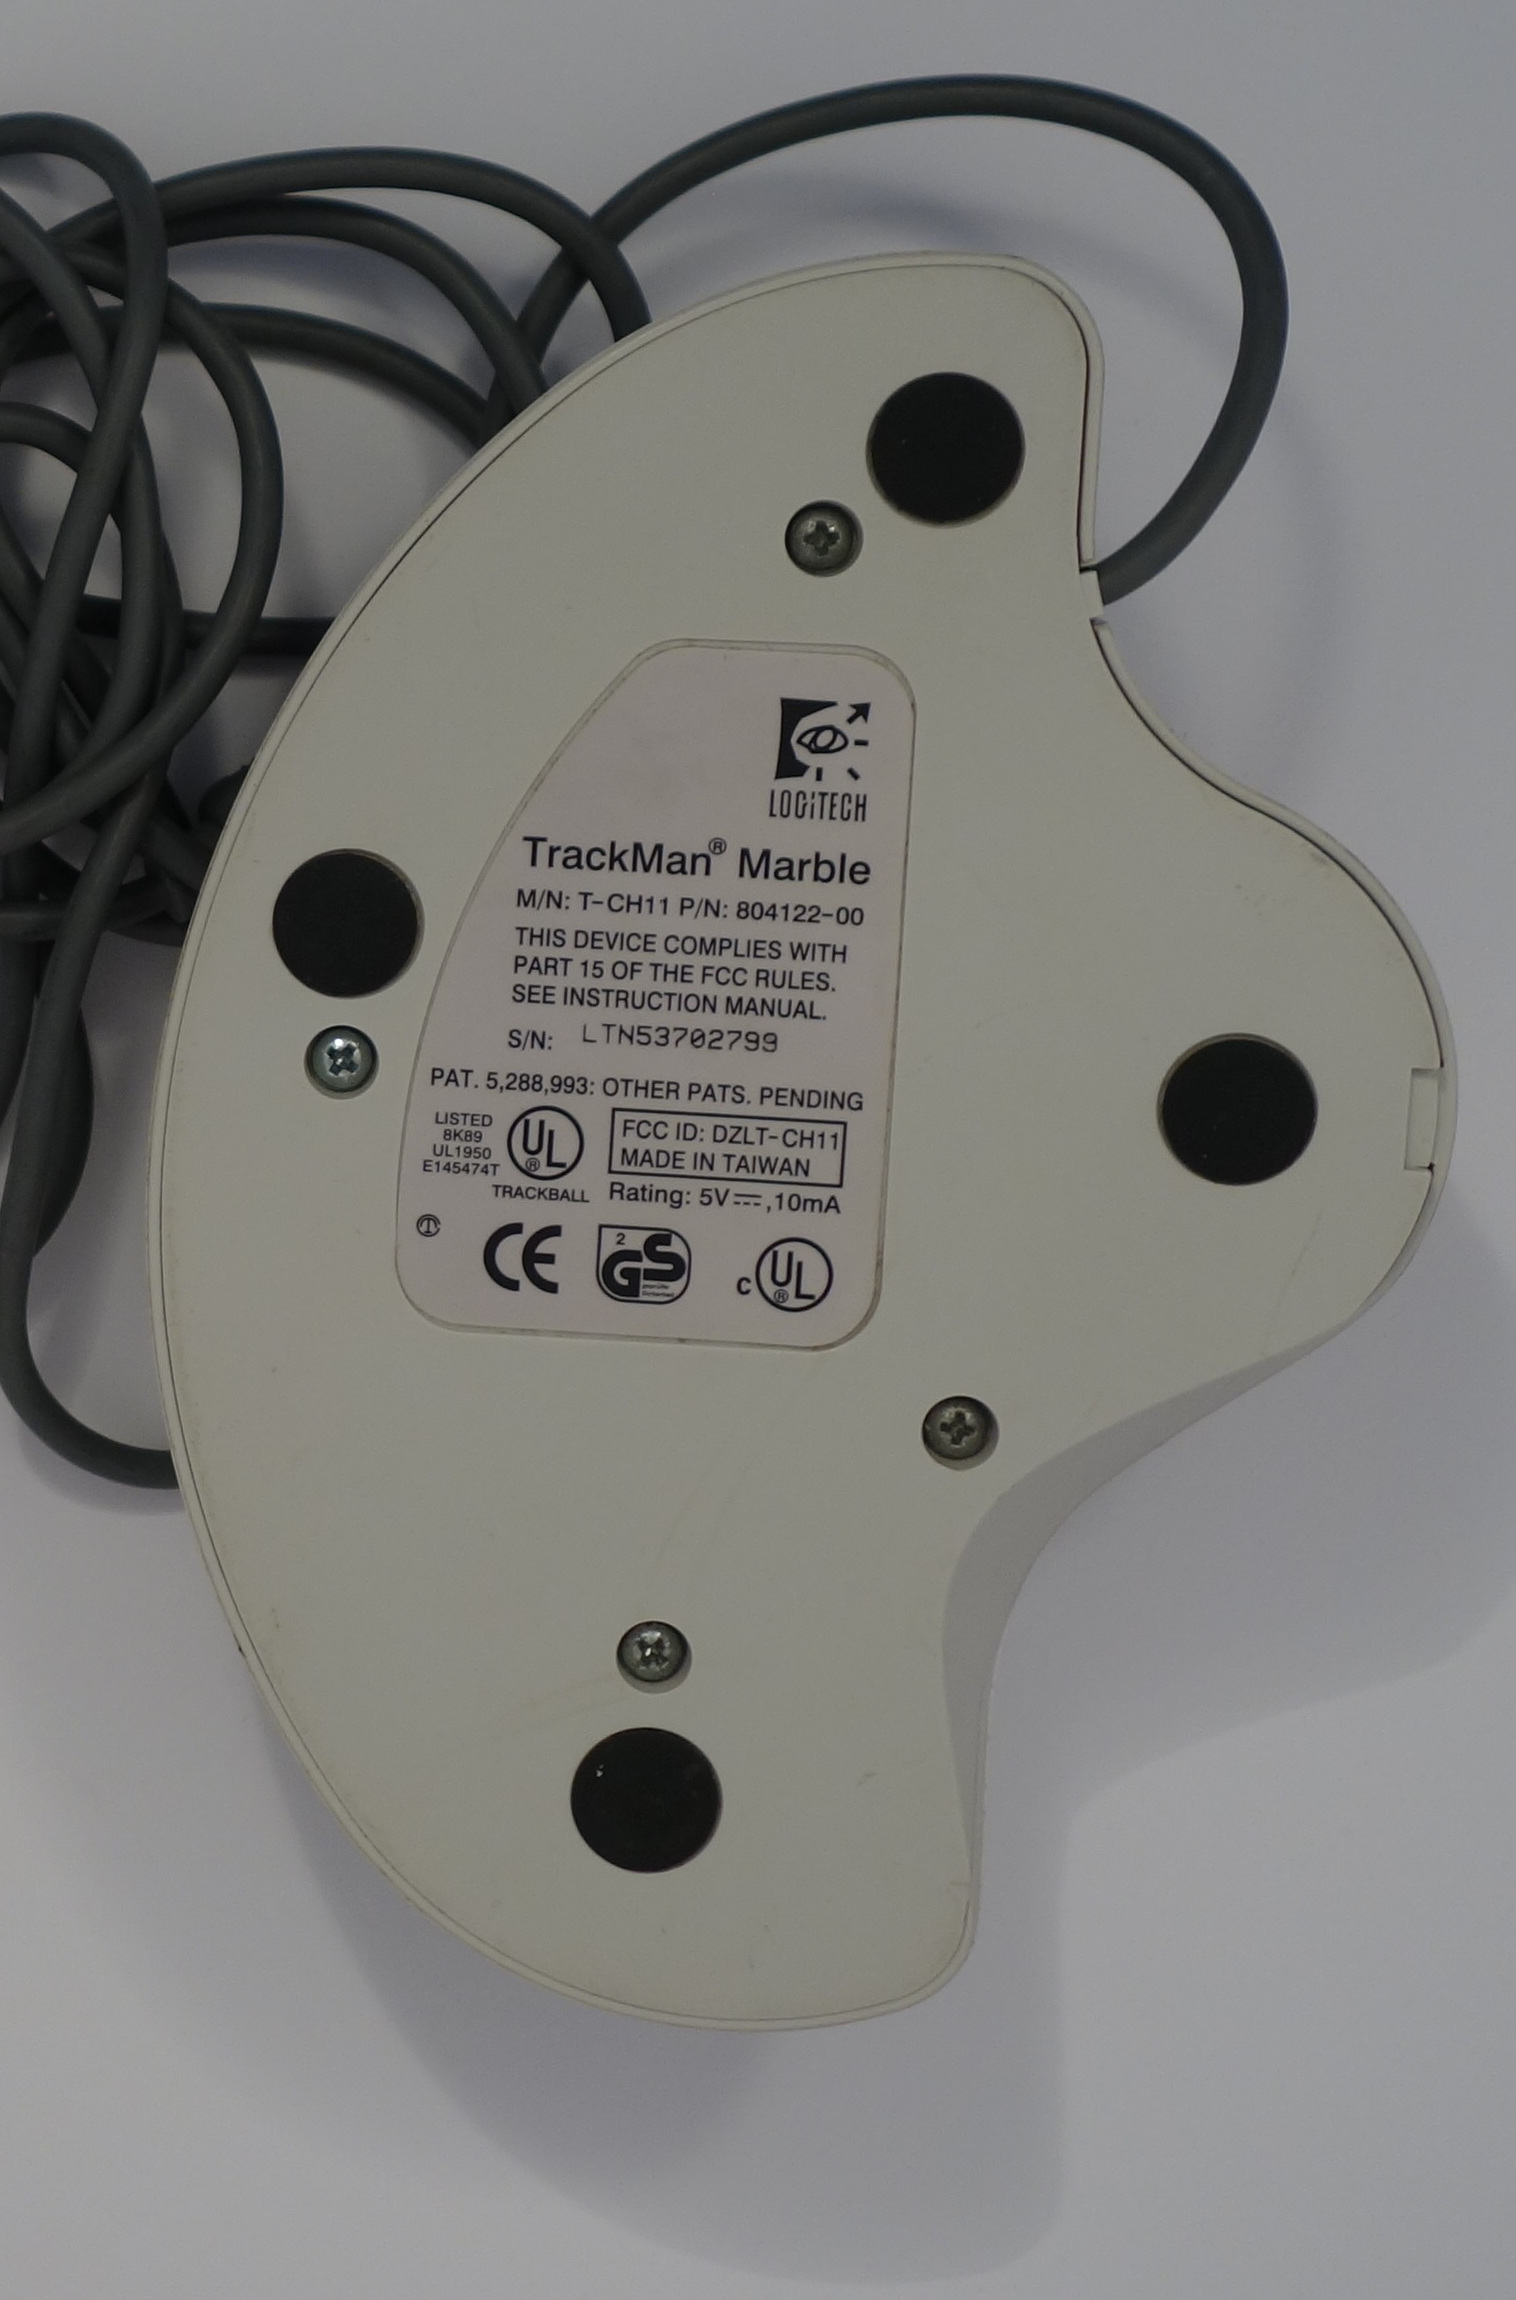
\includegraphics[scale=0.5]{1995_logitech_trackman/2.17.JPG}
%    \caption{Изображение Logitech TrackMan вид снизу}
%    \label{fig:trackmanBottom}
%\end{figure}

\begin{thebibliography}{9}
\bibitem{marbleAdv} Melissa J. Perenson. New \& improved. News of announced products and upgrades. // PC Magazine, Vol. 14, No. 22. -- December 19, 1995. -- p. 61 -- 66.
\end{thebibliography}

\end{document}

\documentclass[11pt, a4paper]{article}
\usepackage{pdfpages}
\usepackage{parallel}
\usepackage[T2A]{fontenc}
\usepackage{ucs}
\usepackage[utf8x]{inputenc}
\usepackage[polish,english,russian]{babel}
\usepackage{hyperref}
\usepackage{rotating}
\usepackage[inner=2cm,top=1.8cm,outer=2cm,bottom=2.3cm,nohead]{geometry}
\usepackage{listings}
\usepackage{graphicx}
\usepackage{wrapfig}
\usepackage{longtable}
\usepackage{indentfirst}
\usepackage{array}
\usepackage{tikzsymbols}
\usepackage{soul}
\usepackage[ruled,vlined]{algorithm2e}
%\counterwithout{figure}{section} 

\usepackage{url}
\makeatletter
\g@addto@macro{\UrlBreaks}{\UrlOrds}
\makeatother

\newcolumntype{P}[1]{>{\raggedright\arraybackslash}p{#1}}
\frenchspacing
\usepackage{fixltx2e} %text sub- and superscripts
\usepackage{icomma} % коскі ў матэматычным рэжыме
\PreloadUnicodePage{4}

\newcommand{\longpage}{\enlargethispage{\baselineskip}}
\newcommand{\shortpage}{\enlargethispage{-\baselineskip}}

\def\switchlang#1{\expandafter\csname switchlang#1\endcsname}
\def\switchlangbe{
\let\saverefname=\refname%
\def\refname{Літаратура}%
\def\figurename{Іл.}%
}
\def\switchlangen{
\let\saverefname=\refname%
\def\refname{References}%
\def\figurename{Fig.}%
}
\def\switchlangru{
\let\saverefname=\refname%
\let\savefigurename=\figurename%
\def\refname{Литература}%
\def\figurename{Рис.}%
}

\hyphenation{admi-ni-stra-tive}
\hyphenation{ex-pe-ri-ence}
\hyphenation{fle-xi-bi-li-ty}
\hyphenation{Py-thon}
\hyphenation{ma-the-ma-ti-cal}
\hyphenation{re-ported}
\hyphenation{imp-le-menta-tions}
\hyphenation{pro-vides}
\hyphenation{en-gi-neering}
\hyphenation{com-pa-ti-bi-li-ty}
\hyphenation{im-pos-sible}
\hyphenation{desk-top}
\hyphenation{elec-tro-nic}
\hyphenation{com-pa-ny}
\hyphenation{de-ve-lop-ment}
\hyphenation{de-ve-loping}
\hyphenation{de-ve-lop}
\hyphenation{da-ta-ba-se}
\hyphenation{plat-forms}
\hyphenation{or-ga-ni-za-tion}
\hyphenation{pro-gramming}
\hyphenation{in-stru-ments}
\hyphenation{Li-nux}
\hyphenation{sour-ce}
\hyphenation{en-vi-ron-ment}
\hyphenation{Te-le-pathy}
\hyphenation{Li-nux-ov-ka}
\hyphenation{Open-BSD}
\hyphenation{Free-BSD}
\hyphenation{men-ti-on-ed}
\hyphenation{app-li-ca-tion}

\def\progref!#1!{\texttt{#1}}
\renewcommand{\arraystretch}{2} %Іначай формулы ў матрыцы зліпаюцца з лініямі
\usepackage{array}

\def\interview #1 (#2), #3, #4, #5\par{

\section[#1, #3, #4]{#1 -- #3, #4}
\def\qname{LVEE}
\def\aname{#1}
\def\q ##1\par{{\noindent \bf \qname: ##1 }\par}
\def\a{{\noindent \bf \aname: } \def\qname{L}\def\aname{#2}}
}

\def\interview* #1 (#2), #3, #4, #5\par{

\section*{#1\\{\small\rm #3, #4. #5}}
\ifx\ParallelWhichBox\undefined%
    \addcontentsline{toc}{section}{#1, #3, #4}%
\else%
\ifnum\ParallelWhichBox=0%
    \addcontentsline{toc}{section}{#1, #3, #4}%
\fi\fi%

\def\qname{LVEE}
\def\aname{#1}
\def\q ##1\par{{\noindent \bf \qname: ##1 }\par}
\def\a{{\noindent \bf \aname: } \def\qname{L}\def\aname{#2}}
}

\newcommand{\interviewfooter}[1]{
\vskip 1em
\noindent \textit{#1}
}


\begin{document}

\title{1996 "--- Kensington Expert Mouse Trackball 5.0}

\maketitle
В 1996 году с выходом пятой по счёту модели Expert Mouse Trackball претерпел существенный редизайн \cite{KensingtonPC}. Устройство оснащено крупным шаром и четырьмя крупными кнопками, расположенными вокруг него как лепестки цветка (рис. \ref{fig:pic}).

\begin{figure}[h]
    \centering
    \includegraphics[scale=0.4]{1996_kensington_expert_trackball_5/king.jpg}
    \caption{Kensington Expert Trackball}
    \label{fig:pic}
\end{figure}

Аналогично выглядевшая версия для Macintosh с предсказуемым названием Turbo Mouse 5.0 (\cite{KensingtonMac}) отличалась интерфейсом ADB, в то время как Expert Mouse комплектовался сменными кабелями для подключения к последовательному интерфейсу и к порту PS/2 (также отдельно выпускалась шинная версия с ISA-адаптером). Визуально устройства не отличались.

\begin{figure}[h]
    \centering
    \includegraphics[scale=0.5]{1996_kensington_expert_trackball_5/kingup.JPG}
    \includegraphics[scale=0.5]{1996_kensington_expert_trackball_5/kingdown.JPG}
    \caption{Kensington Expert Trackball вид сверху}
    \label{fig:top}
\end{figure}



%\begin{figure}[h]
%    \centering
%    \includegraphics[scale=0.2]{1996_kensington_expert_trackball_5/234.JPG}
%    \caption{Kensington Expert Trackball вид снизу}
%    \label{fig:bottom}
%\end{figure}


\begin{figure}[h]
    \centering
    \includegraphics[scale=0.3]{1996_kensington_expert_trackball_5/kingset.jpg}
    \caption{Kensington Expert Trackball на размерном коврике с шагом сетки 1~см}
    \label{fig:size}
\end{figure}


\begin{figure}[h]
    \centering
    \includegraphics[scale=0.3]{1996_kensington_expert_trackball_5/kingset2.jpg}
    \caption{Изображение Kensington Expert Trackball с моделью руки человека}
    \label{fig:hand}
\end{figure}

Это удобно, например для изготовления снимков области экрана или других прецизионных действий — обеспечивается точность до пикселя. Поначалу немного неудобно вращать шар, не отпуская кнопку (ну, например, для выделения текста или объектов на экране), но это дело привычки. 

\begin{figure}[h]
    \centering
    \includegraphics[scale=0.4]{1996_kensington_expert_trackball_5/king2.jpg}
    \caption{Kensington Expert Trackball в разобранном виде}
    \label{fig:inside}
\end{figure}

Внутреннее устройство данного трекбола показано на рисунке 2.21, что позволяет классифицировать трекбол как оптомеханический.

\begin{thebibliography}{9}

\bibitem {KensingtonPC} Kensington: Expert Mouse 5.0 "--- \url{https://web.archive.org/web/19970106170305/http://www.kensington.com/prod/mice/mice3b.html}
\bibitem {KensingtonMac} Kensington: Turbo Mouse 5.0 "--- \url{https://web.archive.org/web/19970106170317/http://www.kensington.com/prod/mice/mice3a.html}
\end{thebibliography}

\end{document}

\documentclass[11pt, a4paper]{article}
\usepackage{pdfpages}
\usepackage{parallel}
\usepackage[T2A]{fontenc}
\usepackage{ucs}
\usepackage[utf8x]{inputenc}
\usepackage[polish,english,russian]{babel}
\usepackage{hyperref}
\usepackage{rotating}
\usepackage[inner=2cm,top=1.8cm,outer=2cm,bottom=2.3cm,nohead]{geometry}
\usepackage{listings}
\usepackage{graphicx}
\usepackage{wrapfig}
\usepackage{longtable}
\usepackage{indentfirst}
\usepackage{array}
\usepackage{tikzsymbols}
\usepackage{soul}
\usepackage[ruled,vlined]{algorithm2e}
%\counterwithout{figure}{section} 

\usepackage{url}
\makeatletter
\g@addto@macro{\UrlBreaks}{\UrlOrds}
\makeatother

\newcolumntype{P}[1]{>{\raggedright\arraybackslash}p{#1}}
\frenchspacing
\usepackage{fixltx2e} %text sub- and superscripts
\usepackage{icomma} % коскі ў матэматычным рэжыме
\PreloadUnicodePage{4}

\newcommand{\longpage}{\enlargethispage{\baselineskip}}
\newcommand{\shortpage}{\enlargethispage{-\baselineskip}}

\def\switchlang#1{\expandafter\csname switchlang#1\endcsname}
\def\switchlangbe{
\let\saverefname=\refname%
\def\refname{Літаратура}%
\def\figurename{Іл.}%
}
\def\switchlangen{
\let\saverefname=\refname%
\def\refname{References}%
\def\figurename{Fig.}%
}
\def\switchlangru{
\let\saverefname=\refname%
\let\savefigurename=\figurename%
\def\refname{Литература}%
\def\figurename{Рис.}%
}

\hyphenation{admi-ni-stra-tive}
\hyphenation{ex-pe-ri-ence}
\hyphenation{fle-xi-bi-li-ty}
\hyphenation{Py-thon}
\hyphenation{ma-the-ma-ti-cal}
\hyphenation{re-ported}
\hyphenation{imp-le-menta-tions}
\hyphenation{pro-vides}
\hyphenation{en-gi-neering}
\hyphenation{com-pa-ti-bi-li-ty}
\hyphenation{im-pos-sible}
\hyphenation{desk-top}
\hyphenation{elec-tro-nic}
\hyphenation{com-pa-ny}
\hyphenation{de-ve-lop-ment}
\hyphenation{de-ve-loping}
\hyphenation{de-ve-lop}
\hyphenation{da-ta-ba-se}
\hyphenation{plat-forms}
\hyphenation{or-ga-ni-za-tion}
\hyphenation{pro-gramming}
\hyphenation{in-stru-ments}
\hyphenation{Li-nux}
\hyphenation{sour-ce}
\hyphenation{en-vi-ron-ment}
\hyphenation{Te-le-pathy}
\hyphenation{Li-nux-ov-ka}
\hyphenation{Open-BSD}
\hyphenation{Free-BSD}
\hyphenation{men-ti-on-ed}
\hyphenation{app-li-ca-tion}

\def\progref!#1!{\texttt{#1}}
\renewcommand{\arraystretch}{2} %Іначай формулы ў матрыцы зліпаюцца з лініямі
\usepackage{array}

\def\interview #1 (#2), #3, #4, #5\par{

\section[#1, #3, #4]{#1 -- #3, #4}
\def\qname{LVEE}
\def\aname{#1}
\def\q ##1\par{{\noindent \bf \qname: ##1 }\par}
\def\a{{\noindent \bf \aname: } \def\qname{L}\def\aname{#2}}
}

\def\interview* #1 (#2), #3, #4, #5\par{

\section*{#1\\{\small\rm #3, #4. #5}}
\ifx\ParallelWhichBox\undefined%
    \addcontentsline{toc}{section}{#1, #3, #4}%
\else%
\ifnum\ParallelWhichBox=0%
    \addcontentsline{toc}{section}{#1, #3, #4}%
\fi\fi%

\def\qname{LVEE}
\def\aname{#1}
\def\q ##1\par{{\noindent \bf \qname: ##1 }\par}
\def\a{{\noindent \bf \aname: } \def\qname{L}\def\aname{#2}}
}

\newcommand{\interviewfooter}[1]{
\vskip 1em
\noindent \textit{#1}
}


\begin{document}

\title{1997 "--- Fellowes Sphere Trackball}
\date{}
\maketitle
Fellowes Sphere Trackball — типичный представитель данного типа указательных устройств ввода информации для компьютера, наиболее характерных для первой половины 90-х годов (хотя и выпущен компанией Fellowes Computerware в 1997). Поскольку трекбол аналогичен мыши по принципу действия и по функциям, но появился раньше, чем мышь, широко распространено мнение, что мышь была изобретена путем переворачивания трекбола вверх дном и его перемещения по поверхности стола.

\begin{figure}[h]
    \centering
    \includegraphics[scale=0.2]{1997_fellowes_trackball/fellowes.jpg}
    \caption{Fellowes Trackball}
    \label{fig:pic}
\end{figure}

Конструктивно трекбол также похож на мышь: вращение шарика приводит в движение пару валиков, соединённых с механическими датчиками, либо, в варианте, появившемся позднее данного, движения шара сканируют размещённые в корпусе оптические датчики. 

\begin{figure}[h]
    \centering
    \includegraphics[scale=0.3]{1997_fellowes_trackball/fellowes2.jpg}
    \caption{Fellowes Trackball в разобранном виде}
    \label{fig:inside}
\end{figure}

Протокол обмена данными между трекболом и компьютером, как правило, также полностью соответствует протоколу для мыши. Поэтому с точки зрения компьютера трекбол является стандартным интерфейсным указательным устройством; в отсутствие специальных драйверов он воспринимаются операционной системой компьютера как стандартная мышь и нормально поддерживаются стандартным универсальным драйвером мыши. 

\begin{figure}[h]
    \centering
    \includegraphics[scale=0.3]{1997_fellowes_trackball/fellowsup.JPG}
    \includegraphics[scale=0.3]{1997_fellowes_trackball/fellowsdown.JPG}
    \caption{Fellowes Trackball, вид сверху и снизу}
    \label{fig:top}
\end{figure}

При работе с трекболом для операций перемещения курсора используется только кисть руки и движения пальцев. Поэтому от пользователя не требуется движений плеча и предплечья, тогда как те же операции с мышью требуют задействования практически всей руки. 
  Поэтому трекбол часто рекомендуется пользователям, испытывающим временные или постоянные проблемы, связанные сплечевым поясом или запястьем.

\begin{figure}[h]
    \centering
    \includegraphics[scale=0.3]{1997_fellowes_trackball/fellowset2.jpg}
    \caption{Fellowes Trackball с моделью руки человека}
    \label{fig:hand}
\end{figure}

В графических приложениях, где позиционирование является основной операцией, использование трекбола, по результатам некоторых исследований, приводит к существенно меньшей усталости и большей точности позиционирования курсора. 

С другой стороны, применение трекбола вместо мыши увеличивает количество движений пальцами, которые вращают шарик, что при активной работе может приводить уже к утомлению пальцев. Также есть сведения, что треболы с шаром, расположенным под большим палцем, способны при длительной и напряженной эксплуатации приводить к проблемам суставов большого пальца.


%\begin{figure}[h]
%    \centering
%    
%    \caption{Fellowes Trackball вид снизу}
%    \label{fig:bottom}
%\end{figure}

\begin{figure}[h]
    \centering
    \includegraphics[scale=0.25]{1997_fellowes_trackball/fellowsset.jpg}
    \caption{Fellowes Trackball на размерном коврике с шагом сетки 1~см}
    \label{fig:size}
\end{figure}

Трекбол не требует пространства на рабочем месте, превышающего собственные размеры, его даже можно жёстко закрепить (в том числе на негоризонтальной поверхности), гарантировав, что он случайно не переместится, не упадёт с рабочего места. В условиях ограниченного пространства или необходимости работать в неудобных положениях это может быть решающим аргументом.

Производитель трекбола в рекламных материалах делал упор на высококачественные кнопки большой площади, а также симметричный дизайн, одинаково удобный как для левой, так и для правой руки. В плане совместимости заявлена поддержка ОС Windows начиная с версии 3.1.


\documentclass[11pt, a4paper]{article}
\usepackage{pdfpages}
\usepackage{parallel}
\usepackage[T2A]{fontenc}
\usepackage{ucs}
\usepackage[utf8x]{inputenc}
\usepackage[polish,english,russian]{babel}
\usepackage{hyperref}
\usepackage{rotating}
\usepackage[inner=2cm,top=1.8cm,outer=2cm,bottom=2.3cm,nohead]{geometry}
\usepackage{listings}
\usepackage{graphicx}
\usepackage{wrapfig}
\usepackage{longtable}
\usepackage{indentfirst}
\usepackage{array}
\usepackage{tikzsymbols}
\usepackage{soul}
\usepackage[ruled,vlined]{algorithm2e}
%\counterwithout{figure}{section} 

\usepackage{url}
\makeatletter
\g@addto@macro{\UrlBreaks}{\UrlOrds}
\makeatother

\newcolumntype{P}[1]{>{\raggedright\arraybackslash}p{#1}}
\frenchspacing
\usepackage{fixltx2e} %text sub- and superscripts
\usepackage{icomma} % коскі ў матэматычным рэжыме
\PreloadUnicodePage{4}

\newcommand{\longpage}{\enlargethispage{\baselineskip}}
\newcommand{\shortpage}{\enlargethispage{-\baselineskip}}

\def\switchlang#1{\expandafter\csname switchlang#1\endcsname}
\def\switchlangbe{
\let\saverefname=\refname%
\def\refname{Літаратура}%
\def\figurename{Іл.}%
}
\def\switchlangen{
\let\saverefname=\refname%
\def\refname{References}%
\def\figurename{Fig.}%
}
\def\switchlangru{
\let\saverefname=\refname%
\let\savefigurename=\figurename%
\def\refname{Литература}%
\def\figurename{Рис.}%
}

\hyphenation{admi-ni-stra-tive}
\hyphenation{ex-pe-ri-ence}
\hyphenation{fle-xi-bi-li-ty}
\hyphenation{Py-thon}
\hyphenation{ma-the-ma-ti-cal}
\hyphenation{re-ported}
\hyphenation{imp-le-menta-tions}
\hyphenation{pro-vides}
\hyphenation{en-gi-neering}
\hyphenation{com-pa-ti-bi-li-ty}
\hyphenation{im-pos-sible}
\hyphenation{desk-top}
\hyphenation{elec-tro-nic}
\hyphenation{com-pa-ny}
\hyphenation{de-ve-lop-ment}
\hyphenation{de-ve-loping}
\hyphenation{de-ve-lop}
\hyphenation{da-ta-ba-se}
\hyphenation{plat-forms}
\hyphenation{or-ga-ni-za-tion}
\hyphenation{pro-gramming}
\hyphenation{in-stru-ments}
\hyphenation{Li-nux}
\hyphenation{sour-ce}
\hyphenation{en-vi-ron-ment}
\hyphenation{Te-le-pathy}
\hyphenation{Li-nux-ov-ka}
\hyphenation{Open-BSD}
\hyphenation{Free-BSD}
\hyphenation{men-ti-on-ed}
\hyphenation{app-li-ca-tion}

\def\progref!#1!{\texttt{#1}}
\renewcommand{\arraystretch}{2} %Іначай формулы ў матрыцы зліпаюцца з лініямі
\usepackage{array}

\def\interview #1 (#2), #3, #4, #5\par{

\section[#1, #3, #4]{#1 -- #3, #4}
\def\qname{LVEE}
\def\aname{#1}
\def\q ##1\par{{\noindent \bf \qname: ##1 }\par}
\def\a{{\noindent \bf \aname: } \def\qname{L}\def\aname{#2}}
}

\def\interview* #1 (#2), #3, #4, #5\par{

\section*{#1\\{\small\rm #3, #4. #5}}
\ifx\ParallelWhichBox\undefined%
    \addcontentsline{toc}{section}{#1, #3, #4}%
\else%
\ifnum\ParallelWhichBox=0%
    \addcontentsline{toc}{section}{#1, #3, #4}%
\fi\fi%

\def\qname{LVEE}
\def\aname{#1}
\def\q ##1\par{{\noindent \bf \qname: ##1 }\par}
\def\a{{\noindent \bf \aname: } \def\qname{L}\def\aname{#2}}
}

\newcommand{\interviewfooter}[1]{
\vskip 1em
\noindent \textit{#1}
}


\begin{document}

\title{1998 "--- Apple Puck Mouse}
\date{}
\maketitle
Мышь Apple USB mouse, часто называемая <<шайбой>> (англ. <<puck>>)  из-за своей необычной формы, была разработана компанией Apple в 1998 году. Это была первая коммерчески выпущенная мышь Apple mouse, которая использовала формат подключения USB, а не шину Apple ADB. Многие обозреватели критиковали данную мышь за ее недостаточно эргономичный дизайн.

\begin{figure}[h]
    \centering
    \includegraphics[scale=0.6]{1998_apple_puck/apple60.jpg}
    \caption{Apple Puck Mouse}
    \label{fig:pic}
\end{figure}

В отличие от большинства манипуляторов, эта мышь имеет круглую форму, и у нее есть одна кнопка, расположенная вверху, как и у предыдущих мышей Apple. При этом мышь имеет зазор между кнопкой и корпусом, показывающий, куда именно пользователь должен нажимать \cite{Apple}.

\begin{figure}[h]
    \centering
    \includegraphics[scale=0.6]{1998_apple_puck/appleup60.jpg}
    \includegraphics[scale=0.6]{1998_apple_puck/appledown60.jpg}
    \caption{Apple Puck Mouse, вид сверху и снизу}
    \label{fig:top}
\end{figure}

Круглая форма мыши была признана сообществом неудобной из-за небольшого размера данного конкретного манипулятора и склонности вращаться при использовании.
Также из-за малого размера, перемещение мыши на самом деле требовало гораздо большего количества движений  пальцев и  меньшего количества движений запястья по сравнению с более крупными мышами (рис. \ref{fig:size}, \ref{fig:hand}).

\begin{figure}[h]
    \centering
    \includegraphics[scale=0.3]{1998_apple_puck/appleset60.jpg}
    \caption{Apple Puck Mouse на размерном коврике с шагом сетки 1~см}
    \label{fig:size}
\end{figure}

\begin{figure}[h]
    \centering
    \includegraphics[scale=0.3]{1998_apple_puck/appleset62.jpg}
    \caption{Apple Puck Mouse с моделью руки человека}
    \label{fig:hand}
\end{figure}

Это стало основной причиной успеха адаптеров-накладок, таких как iCatch Mouse Adapter \cite{bib:icatch}, придававших мыши более продолговатую форму (рис. \ref{fig:addon}

\begin{figure}[h]
    \centering
    \includegraphics[scale=0.6]{1998_apple_puck/apple63.jpg}
    \includegraphics[scale=0.6]{1998_apple_puck/appleup63.JPG}
    \includegraphics[scale=0.6]{1998_apple_puck/appledown63.JPG}
    \caption{Apple Puck Mouse, вид с накладкой}
    \label{fig:addon}
\end{figure}



В полупрозрачном пластике помещалась печатная плата и двухцветный шар, который можно было легко разглядеть. 


Однако идеально круглое тело часто приводило к ошибкам, так как пользователи предполагали, что мышь была в правильной ориентации, даже если это было не так. Позже Apple добавила ямочку на корпусе мыши, чтобы помочь пользователям почувствовать, в каком направлении указывала мышь.
\begin{figure}[h]
    \centering
    \includegraphics[scale=0.6]{1998_apple_puck/apple62.jpg}
    \caption{Apple Puck Mouse, в разобранном виде}
    \label{fig:inside}
\end{figure}

Внутреннее устройство данной мыши показано на рис. \ref{fig:inside}, что позволяет классифицировать  ее как оптомеханическую.

\begin{thebibliography}{9}

    \bibitem {Apple} An ode to the puck, Apple's first USB mouse "--- \url{https://thehouseofmoth.com/an-ode-to-the-puck-apples-first-usb-mouse/} 
    \bibitem{icatch} The iCatch Mouse Adapter \url{https://web.archive.org/web/20001024170633/http://www.macsensetech.com:80/Product/iCatch.html}
\end{thebibliography}

\end{document}

\newpage

\makeatletter
\let\enddocument\@lvee@enddoc
\let\input\@lvee@input
\makeatother

\eof

